\chapter{Texture Reconstruction}
\label{chapter:texture-recon}
In this chapter, we mainly study the texture reconstruction problem in two different ways. Section~\ref{sec:toptim} presents \emph{3DLite} that produces abstracted scene with completed planar geometry with high-quality texture. Section~\ref{sec:tadv} discusses a novel method that jointly optimize the texture with an adversarial learned metric that tolerates scanning errors.

\section{Texture Optimization with Explicit Model}
\label{sec:toptim}

\subsection{Overview}
\begin{figure}
	\centering
	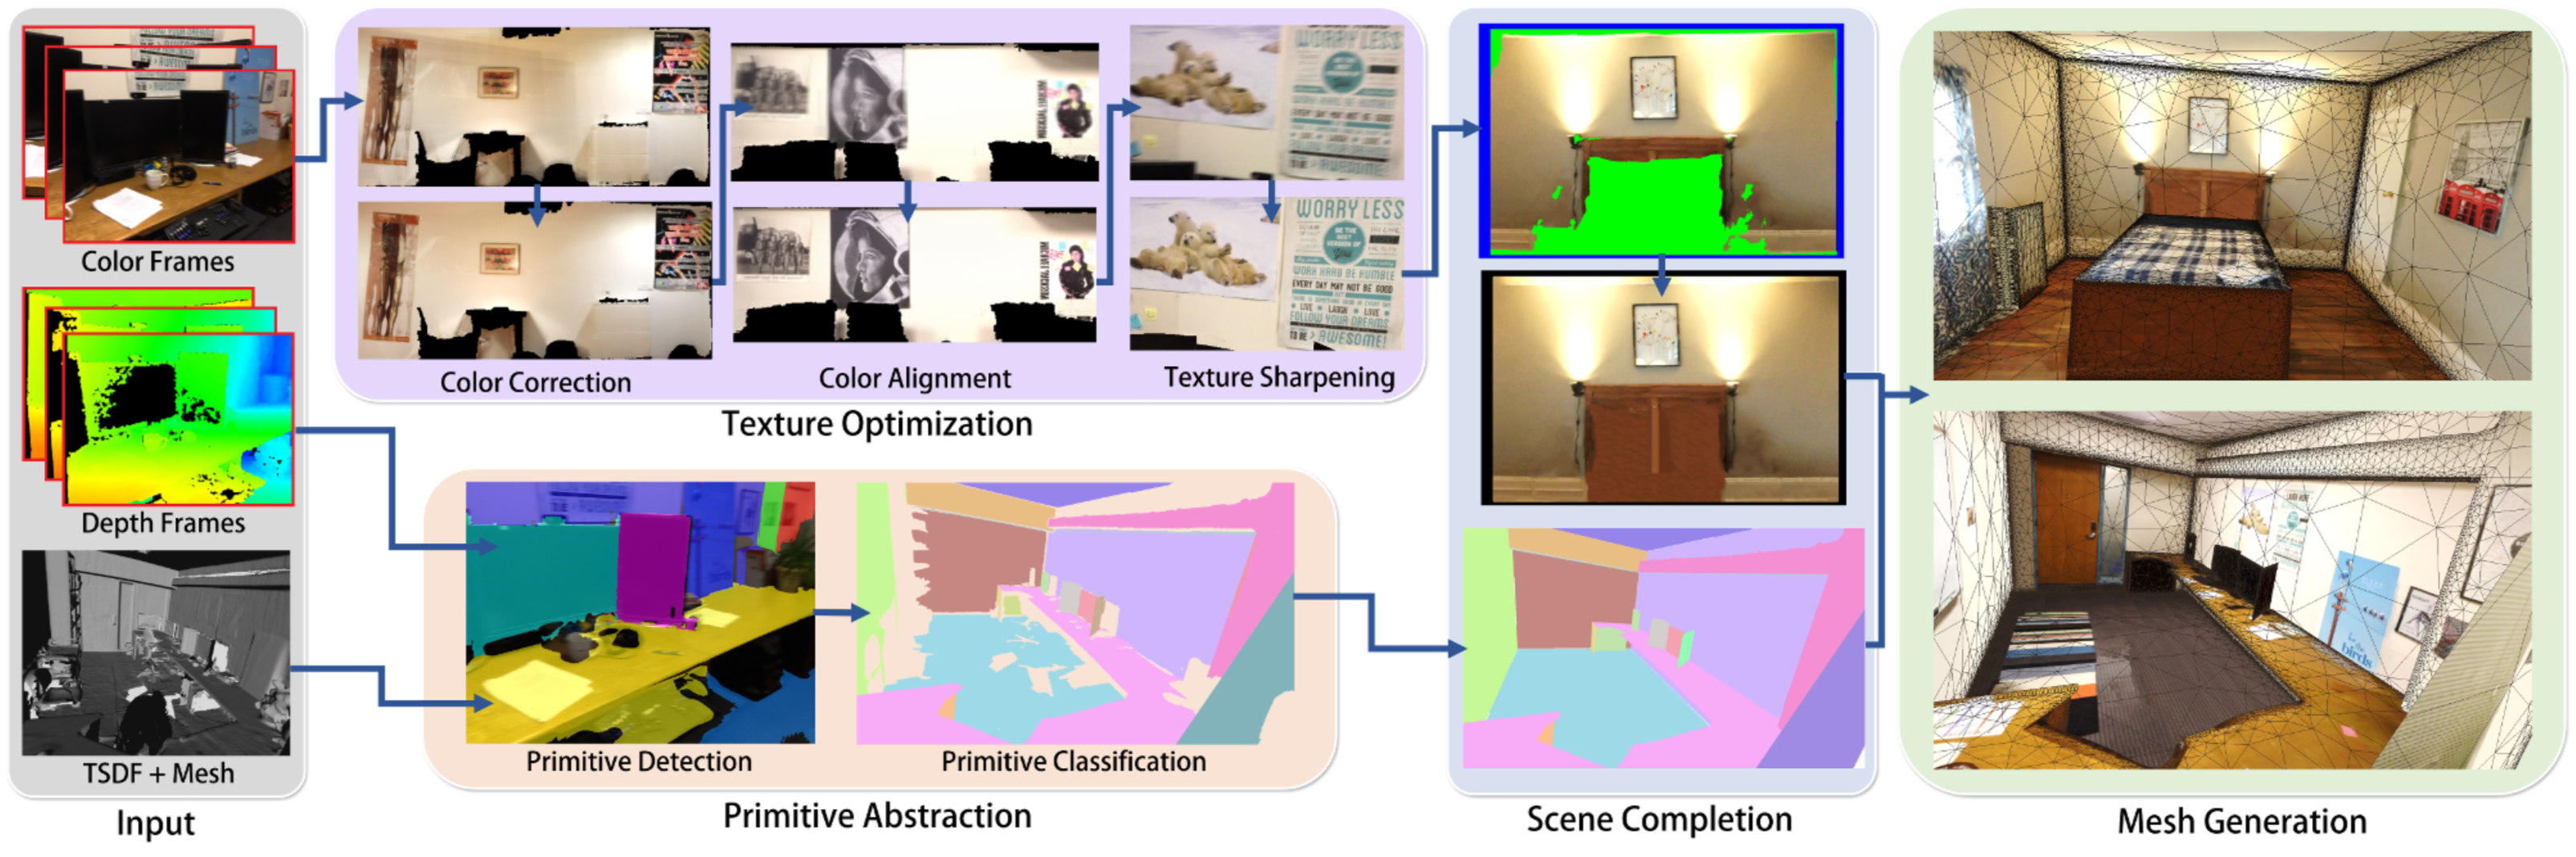
\includegraphics[width=\textwidth]{3dlite/fig2.png}
	\caption{Framework overview: our method takes a set of RGB-D frames as input, from which we compute a primitive abstraction that is used to optimize for sharp surface textures and infer missing scene parts. In the end, we obtain a low-polygonal, lightweight 3D reconstruction.
	}
%	\vspace{-0.2cm}	
	\label{fig:3dlite-overview}
\end{figure}
From an input RGB-D video, 3DLite\footnote{This section is mainly based on our work~\cite{huang20173dlite}.} first computes a primitive-based abstraction of the scene, and then leverages this representation to optimize for high-quality texture maps, as well as complete holes in the scene with both geometry and color; see Fig.~\ref{fig:3dlite-overview}.
We capture the input RGB-D stream with a handheld, consumer-grade RGB-D sensor.
Using a modern RGB-D reconstruction system (i.e., BundleFusion~\cite{dai2016bundlefusion}), we compute initial camera poses for each frame and a truncated signed distance field (TSDF) representation of the scene, from which we extract an initial mesh.
To generate the primitive-based abstraction, we detect planes for each frame, and then merge them into scene primitives according to the estimated camera poses (see section~\ref{sec:3dlite-plane-abstraction}).
We then optimize for the global geometric structure by favoring primitives to support a Manhattan world assumption, so as to encourage orthogonal and parallel structures.

From this lightweight representation of the scene, we then optimize for texture maps over the geometry, directly addressing the issues of motion blur and small camera pose misalignments.
We apply an exposure correction to achieve consistent color across the input images, which may vary with auto-exposure and white balancing (see section.~\ref{subsec:3dlite-color-transfer}).
We must then refine the camera poses to precisely align the color frames to the new model geometry.
To this end, we build upon the approach of Zhou and Koltun~\cite{zhou2014color} to optimize for refined camera poses and non-rigid image corrections.
For our large-scale scanning scenario, we introduce sparse color feature and geometric primitive constraints to help bring the optimization into the basin of convergence of a dense photometric consistency energy (see section~\ref{subsec:3dlite-color-align}).
In order to account for motion blur in input color images, we introduce a method to sharpen color projected from input frames to the model.
Rather than select sharpest keyframes throughout the input video, which may still select relatively blurry frames or lose color information by filtering out too many frames, we seek sharp image regions, from which we formulate a graph-cut based optimization for image sharpness and coherence (see section~\ref{subsec:3dlite-color-sharp}). 
%\angie{plz check this sharpening part} \jingweiNote{Additionally, we select $\triangle I$ from sharpest region, and optimize the final texture combining $\triangle I$ and averaged color. Do we describe it here?}
This leads to a high-quality texture map over the known geometry.

We then complete the textured model to fill holes that were occluded or unseen in the original scan.
While general, high-resolution scene completion is a very challenging task, our primitive-based abstraction enables effective hole-filling for both geometry and color on our scene representation.
To complete the geometry of the model, we extrapolate primitives in unobserved space according to the camera trajectory, such that each primitive meets either another primitive or empty space (see section~\ref{subsec:3dlite-extrapolate}). %\angie{is this actually true? also are we doing things different from dzitsiuk2016noising?} \jingweiNote{We extrapolate two planes to connect them, otherwise we don't extrapolate any plane even if there is unobserved space. Should be similar to dzitsiuk2016noising, but they really don't have a good explanation on this part.}
We then complete the color in these regions through image inpainting, following  Image Melding~\cite{darabi2012image} (see section~\ref{subsec:3dlite-inpaint}).
This produces a clean, complete, lightweight model mapped with sharp textures.
\section{Primitive-Based Abstraction}
\label{sec:3dlite-plane-abstraction}

To compute our primitive-based abstraction of a scanned scene, we first detect planes for each input frame, then merge these detected planes into a globally consistent set of primitives, and finally perform a structural refinement, optimizing under parallel and orthogonal constraints.

\subsection{Frame-based Plane Detection}
\label{subsec:3dlite-plane-detect}

From an input RGB-D video sequence comprised of a set of depth and color frames $\{f_i = (\mathcal{C}_i, \mathcal{D}_i)\}$, we first use a state-of-the-art RGB-D reconstruction system to obtain initial camera poses $T_i$ (frame-to-world) for each frame, and an initial surface $\mathcal{S}_0$.
For each frame, we detect planes using the fast plane extraction of Feng et al.~\cite{feng2014fast}. 
Instead of detecting planes directly on the input sensor depth, which is noisy and often contains holes, we operate on depth rendered from $\mathcal{S}_0$.
This rendered depth contains data accumulated over previous frames, which regularizes out noise and incorporates more information than a single input depth map, and is also well-aligned to the model geometry $\mathcal{S}_0$.
For each detected plane $\mathcal{P}_k$ in frame $f_i$, we additionally store two terms containing information used for primitive merging and structural refinement, as described in Secs.~\ref{subsec:3dlite-plane-classify} and Sec.~\ref{subsec:3dlite-color-align}.
\begin{itemize}
    \item Plane parameter: $p=(n_x,n_y,n_z,w)$ where $\mathbf{n} = (n_x,n_y,n_z)$ is the unit normal. It represents the plane $\mathbf{n}\cdot \mathbf{x} + w=0$ in the camera space of $f_i$. 
    \item Distance Matrix: $\mathbf{D} = \frac{1}{N}\sum_{q} x_qx_q^T$, where $x_q$ is the world space position of the $q$-th pixel in the depth map. 
    We can then easily compute the average of square point-plane distances (ASD) of $\mathcal{P}_k$ with another plane $\mathcal{P}_l$ in frame $f_j$ as $(p_l^jT_j^{-1})\cdot \mathbf{D}\cdot (p_l^jT_j^{-1})^T$. 
\end{itemize}

\subsection{Primitive Classification}
\label{subsec:3dlite-plane-classify}

We need to aggregate the per-frame planar regions into a set of plane primitives representing the planes in the 3D scene.
Two planar regions $\mathcal{P}_k$ from frame $f_i$ and $\mathcal{P}_l$ from frame $f_j$ are determined to be the same primitive if they are close and have enough overlap. 
We consider $\mathcal{P}_k$ and $\mathcal{P}_l$ to be close if $\max(\textrm{ASD}_{k\rightarrow l}, \textrm{ASD}_{l\rightarrow k}) < \tau_c$ (in practice, we use $\tau_c = 0.05$m).
Overlap is computed by transforming $\mathcal{P}_k$ and into the camera space of $f_j$ and computing the percentage of overlapping pixels relative to the minimum number of pixels belonging to $\mathcal{P}_k$ and $\mathcal{P}_l$.
If this overlap percentage is greater than $\tau_o$ (we use $\tau_o = 0.3$), the regions are considered to overlap.

We perform this merging step hierarchically.
For key frames at interval $n = 10$ frames, we merge planes within each key frames' set of $n$ frames, and then merge planes among all key frames.
Each frame then contains a set of plane primitives labeled according to the resulting merged set.
By projecting the merged primitive labels from the frames onto $\mathcal{S}_0$, we obtain a primitive decomposition of the scene. 
Note that regions with multiple different primitive label assignments (typically occurring near intersections of different primitive) are removed from the primitive set.
Fig.~\ref{fig:3dlite-plane-classify} shows an example primitive decomposition of an office scan, with different primitive denoted by different colors, and gray denoting no label assignment.
 
\begin{figure}
    \centering
    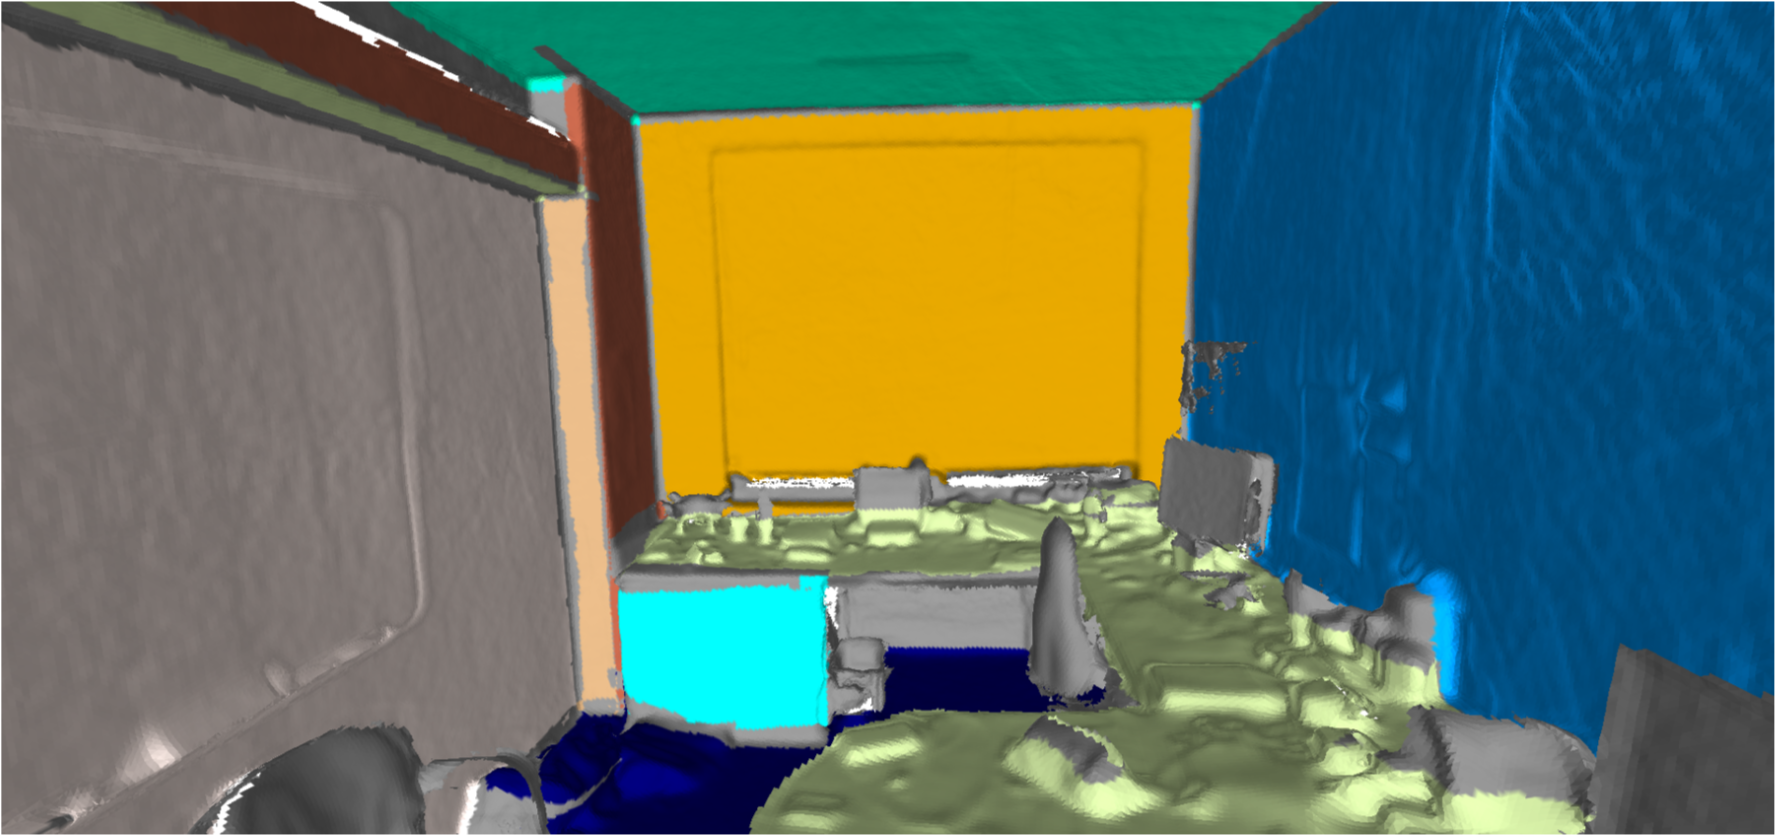
\includegraphics[width=0.97\linewidth]{3dlite/fig3.png}
    \caption{
    	Primitive decomposition: each plane primitive is denoted with a different color. Gray indicates no primitive association.
    }
    \label{fig:3dlite-plane-classify}

\end{figure}

To filter out any potential outliers from the primitive classification projection onto $\mathcal{S}_0$, we filter out small plane primitives (area less than $0.2$m$^2$) and use a RANSAC approach to filter out outlier points of larger primitives.
For a plane primitive $\mathcal{P}_k$, we check for outliers by randomly selecting $3$ of its associated vertices in $\mathcal{S}_0$ and fitting a plane $\mathcal{P}_k'$ to these vertices. 
A point is then considered an inlier for $\mathcal{P}_k'$ if its distance is smaller than $\tau_i$. 
Since $\mathcal{S}_0$ often contains warping in large plane primitives due to sensor noise and distortion, as well as camera pose micro-drift, we conservatively set $\tau_i = 0.1$m.
We repeat this process for $128$ iterations, and update $\mathcal{P}_k$ with the best fitting plane to the largest set of inliers in the least squares sense.

\subsubsection{Structural Refinement}
\label{sec:fit-refine}

Since we use a relatively conservative inlier threshold to compute the plane primitives, planes which should be orthogonal or parallel to each other are typically off by a few degrees.
We thus perform a structure refinement optimization on the planar primitives to encourage them to conform to a Manhattan world.
Similar to Halber and Funkhouser~\cite{halber2016fine}, we formulate an energy minimization using parallel and orthogonal constraints:

\begin{align}
	E_s &= E_d + \lambda E_a\, \\
    E_d &= \sum_{i}^{\#\textrm{planes}} \sum_{j}^{\#\textrm{plane verts}} D(\mathcal{P}_i,v_{ij})^2\,,\\
    E_a &= \sum_{i,j\in \Omega} |A(\mathcal{P}_i,\mathcal{P}_j)-90\cdot n_{ij}|^2\,.
\end{align}

For each plane primitive $\mathcal{P}$, $E_d$ measures the plane fitting error, where $D(\mathcal{P},v_i)$ is the distance from an inlier vertex $v_i$ to $\mathcal{P}$. 
$E_a$ measures the angle error between orthogonal planes, where $A(\mathcal{P}_i,\mathcal{P}_j)$ is the angle of two planes, $\Omega$ is a set of parallel and orthogonal plane pairs. 
The set $\Omega$ is collected by testing each pair of plane primitives, and adding them to the set if the angular difference between their normals lies in $[90n_{ij}-10, 90n_{ij}+10]$, where $n_{ij}\in \{0,1,2,3\}$. 
The final energy $E_s$ is then a linear combination of $E_d$ and $E_a$, with $\lambda=\frac{E_a^0}{E_d^0}$ to balance the plane fitting error and structure error.

The optimization typically converges in about $10$ iterations, with resulting angle errors less than $1^{\circ}$ and plane fitting error about $1.1$ times larger. 
%The angle error of each pair of planes in $\Omega$ is smaller than $1^{\circ}$, while the plane fitting error is about 1.1x bigger. 
As a result, we can rectify the orthogonal structure of the planar primitives with very small trade-off from fitting accuracy.
From this optimized result, we can produce a lightweight, clean mesh $\mathcal{S}_p$ by projecting the vertices of $\mathcal{S}_0$ to their associated primitives, as shown in Fig~\ref{fig:3dlite-plane-fit}(a). 

\subsection{Texture Optimization}
\label{sec:approach-texture}

We aim to map our primitive-abstracted geometric model $\mathcal{S}_p$ with sharp, clear textures to produce a visually compelling 3D model.
It is not suitable to directly project pixels from each color frame to the geometric model, due to the issues of motion blur and camera misalignments.
In our texture optimization step, we directly address these problems with a texture optimization method to solve for refined camera poses and image warping, as well as a texture sharpening step which considers per-pixel image sharpness to solve for globally crisp colors.

\subsubsection{Color-based Primitive Refinement}
\label{subsec:color-plane-refine}
\begin{figure}
    \centering
    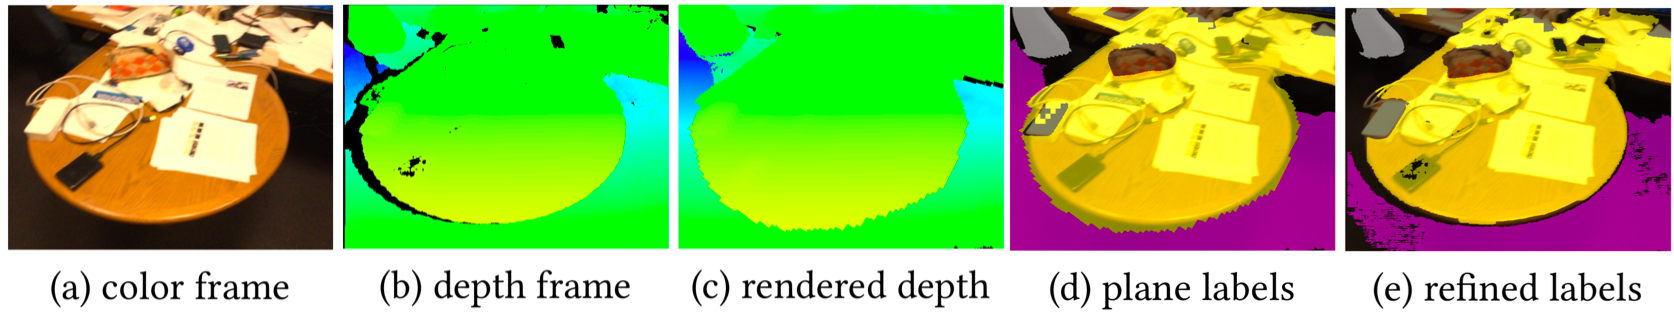
\includegraphics[width=\linewidth]{3dlite/fig4.png}
    \caption{Color-based primitive refinement: (a) Input color. (b) Input depth. (c) Rendered depth. (d) Primitive classification from rendered depth. (e) Refined primitive classification according to the color frame.}
    \label{fig:3dlite-color-boundary-refine}
\end{figure}
Since we originally detected plane primitives from rendered depth (Sec.~\ref{subsec:3dlite-plane-detect}), there may be some disagreement along primitive boundaries with the input RGB-D frame.
Thus pixels that are close to primitive boundaries are easily mis-classified, and we must re-classify them to agree with the input color images. 
To ensure that primitive labels are coherent in the image domain and maintain boundaries consistent with the input color frames, we formulate a graph-cut~\cite{boykov2001fast} based energy minimization problem:
\begin{equation}
E_l = \sum_p D(p, l_p) + \sum_{p,q} V_{pq}\delta(l_p,l_q)\,.
\label{eq:color-boundary-refine}
\end{equation}

Here $D(p,l_p)$ indicates the penalty for pixel $p$ to be classified as $l_p$. 
For confident regions, we won't change their labels $l_p^0$. 
So $D(p,l_p)$ is $1$ for $l_p=l_p^0$ and $\inf$ for other labels. 
For regions that need to be reclassified, $D(p,l_p)=1$ for all labels $l_p$. 
We additionally have a penalty at the boundary of the primitives, $\delta(l_p,l_q)$: $p$ and $q$ are neighbor pixels and $\delta$ is 1 if $l_p\neq l_q$ and 0 otherwise. 
$V_{pq}$ measures how good it is to cut between $p$ and $q$, depending on their color differences. We set
$V_{pq}=e^{\left(||\mathcal{C}(p)-\mathcal{C}(q)||^2\right)/\sigma^2}$.  %$V_{pq}=e^{\frac{||\mathcal{C}(p)-\mathcal{C}(q)||^2}{\sigma^2}}$. 
For our experiments, we re-classify pixels within $10$ pixels of the boundary of a $640\times 480$ image, and use $\sigma=30$ with colors $\mathcal{C}(x)\in[0,255]$.
Figure~\ref{fig:3dlite-color-boundary-refine} shows the result of our refinement.

\subsubsection{Color Transfer Optimization}
\label{subsec:3dlite-color-transfer}
In solving for a texture mapping, it is important to ensure consistent color across different views (e.g., due to auto-white balancing or auto-exposure).
This can be achieved by transferring colors with a mapping function.
For example, NRDC~\cite{hacohen2011non} search for correspondences between images, and optimizes for such a mapping function to transfer color style from one image to another.
In the scenario of RGBD scanning, correspondences can be easily acquired from camera poses and geometry. 
Zhang et al.~\cite{zhang2016emptying} solves the problem by minimizing vertex radiance error viewed from different color frames, given the exposure. 
In order to model white balance and exposure changes, we refer to the NRDC model to transfer colors using three spline curves ($B_j(r,g,b)=(B^1_j(r),B^2_j(g),B^3_j(b))$) for the rgb channels of the $j$-th frame. 
Then for a 3D point $p_i$ and it's corresponding pixels $\{q_{ij}\}$ in frames $\{j\}$ under the current camera poses, we want the color $C(p_i)$ to be close to $B_j(q_{ij})$:
\begin{equation}
E_t = \sum_{i} \sum_{j} ||C(p_i) - B_j(q_{ij})||^2 + \lambda \sum_{i} \sum_{j} (B_j'(x_i)-1)^2\,.
\end{equation}
While \cite{zhang2016emptying} use the first frame as a reference exposure, we don't need this constraint. 
Instead, we regularize the derivatives of the transfer functions $B'_j(x_i)$ to be $\approx 1$. 
This helps preserve the variance of the color. 
We use $\lambda = 0.1$, and $x_i$ is a sequence of 10 integers from 0 to 250 with interval 25.
Since this optimization depends on the quality of the camera transforms, we iterate this color correction step with the color image alignment optimization described below.

\subsubsection{Refined Texture Map Alignment}
\label{subsec:3dlite-color-align}
Key to achieving high-quality texture is obtaining precisely aligned color frames.
This is a challenging task, as there are artifacts from consumer-grade sensors and the geometry is often imprecise.
The color map optimization approach of Zhou and Koltun~\cite{zhou2014color} considers fixed geometry and jointly optimizes for color camera poses and image warping parameters.
This reduces the dimensionality of the problem, using image warping to reduce potential color misalignment from geometric error, achieving compelling results for object scans.
However, their optimization relies on dense photometric error, which has a relatively small basin of convergence and is thus rather sensitive to initial pose estimates.
For our large-scale scanning scenario, this energy is not very robust to the variance in initial camera poses.

In our formulation, we solve for a set of camera parameters for each frame separately from non-rigid correction, which we found to be more effective in practice. 
We adopt the idea of EM optimization with the help of dense color errors from Zhou and Koltun, and solve to maximize photo-consistency.
To aid convergence, we additionally introduce sparse feature and primitive-based constraints into the optimization.
Thus our energy is defined as
$$ E(\mathbf{T})=E_c(\mathbf{T}) + \lambda_s E_s(\mathbf{T}) + \lambda_p E_p(\mathbf{T})\,, $$
where $E_c$ represents the dense photometric energy, $E_s$ the sparse feature term, and $E_p$ primitive relationship constraints, and we solve for rigid camera poses (camera-to-world) $\mathbf{T}=\{T_i\}$ for each frame.
Following Zhou and Koltun, we also optimize for proxy variables $C(p_i)$ denoting the color at 3D point $p_i$ on the geometry surface.
We perform this optimization hierarchically in coarse-to-fine fashion to aid convergence at fine-scale resolution, using 3 hierarchy levels in which $p_i$ are sampled at $0.032$m, $0.008$m, $0.002$m from the primitive-abstracted $\mathcal{S}_p$, respectively.
$\lambda_s$ and $\lambda_p$ are set such that $E_c(\mathbf{T}_0)=\lambda_s E_s(\mathbf{T}_0) = \lambda_p E_p(\mathbf{T}_0)$.

\paragraph*{Sparse Term.}
In our sparse matching term, we minimize the sum of world-space distances between pairs of sparse feature correspondences transformed from image space to the space of the 3D primitives. 
For a frame $f_i$ and plane primitive $\mathcal{P}_k$, we transform a pixel $p_i$ under the homography $H_k^i$, depending on $\mathcal{P}_k$ and the camera pose $T_i$, to bring it into the space of the primitive $\mathcal{P}_k$.
Then for a pixel correspondence $\{p_{im},p_{jm}\}$ from frames $f_i$ and $f_j$ and which correspond to 3D primitives $\mathcal{P}_k$ and $\mathcal{P}_l$ (when projected in 3D under the current camera poses), we optimize for the energy
% Suppose corresponding pixels $p_i$ and $p_j$ are from frames $f(p_i)$ and $f(p_j)$, their distance in the space of the plane will be $H(||\mathbf{T}_{f(p_i)}) p_i - H(\mathbf{T}_{f(p_j)}) p_j||$} \angie{should specify what i and j are in the energy} 
\begin{equation}
E_s(\mathbf{T}) = \sum_m^{\#\textrm{corr}} ||H_k^ip_{im} - H_l^j p_{jm}||^2\,.
\label{eq:pose-optim-sparse}
\end{equation}

Sparse features are detected by projecting each color frame into the plane primitives, detecting SIFT~\cite{lowe2004distinctive} features in the projected images.
Correspondences are determined by SIFT matching followed by a verification step to ascertain that there is a valid 2D rigid transform bringing one set of correspondences from an image to another.
Valid correspondence features are then back-projected to the original color frames to compose the sparse feature set. 
This produces a robust set of feature correspondences, since the projection into a 3D plane does not rely on depth maps which contain noise and distortion, and matching in the warped space contains reduced scale and affine variance than in the original color images.

\paragraph*{Primitive Constraint Term.}
We restrict the per-frame planar regions computed in Sec~\ref{subsec:3dlite-plane-detect} to align well with $\mathcal{S}_p$, geometrically.
\begin{equation}
E_g(\mathbf{T}) = \sum_{i} \sum_{j} (P_j T_j^{-1} p_i)^T (P_j T_j^{-1} p_i)\,.
\label{eq:pose-optim-geo}
\end{equation}
Here, $p_i$ is the homogeneous coordinate of the sampled 3D points from $\mathcal{S}_p$. $P_j$ is the camera-space plane parameter (as in Sec.~\ref{subsec:3dlite-plane-detect}) of the $i$-th planar region of frame $j$.

\paragraph*{Dense Term.} 
Finally, the dense term measures photo-metric error from the color frames projected onto $\mathcal{S}_p$.
\begin{equation}
E_c(\mathbf{T}) = \sum_{i} ||C(p_i) - \sum_j I_j(\pi(T_j^{-1}p_i))||^2\,,
\label{eq:pose-optim-color}
\end{equation} 
where $p_i$ is in the set of sampled 3D points of $\mathcal{S}_p$ and $\pi$ denotes the perspective projection.

We solve for $E(\mathbf{T})$ by solving for both the per-frame transforms $\mathbf{T}$ and the proxy variable colors on the geometry $C(p_i)$.
After an initial three iterations at the coarsest resolution, we are able to compute very reliable sets of correspondences for a color transfer correction (as described in Sec.~\ref{subsec:3dlite-color-transfer}); after the color correction, we further optimize for refined camera poses at the middle and high resolutions for five and two iterations respectively.

%\angie{is this the same as the color map optimization? if so we could just refer to that. otherwise what exactly are the differences?} \jingweiNote{they are exactly the same.}
After solving for the rigid camera poses, we additionally optimize for non-rigid image warping to reduce color misalignment due to possible geometric error, following Zhou and Koltun~\cite{zhou2014color}.
\begin{comment}
Similar to Zhou et al.~\cite{zhou2014color}, we solve for a warping function for each image, $\xi : \mathbb{R}^2\rightarrow \mathbb{R}^2$, which deforms a regular grid $\mathbf{X} = {X_{mn} = (mw,nh)}; m,n\in\mathbb{Z}$ of size $w\times h$ on the image domain.
$\xi(\mathbf{X})$ is then computed as a bilinear interpolation of $\xi(X_{mn})$ at the four nearest grid points.
We then minimize the energy:
\begin{align}
\begin{split}
E_w(\xi) &= \sum_{i} ||C(p_i) - \sum_j I_j(\xi(\pi\cdot T_j^{-1}p_i))||^2 \\
&+ \lambda (||\xi(X_{mn})+(w,0)^T-\xi(X_{m+1,n})||^2\\
& + ||\xi(X_{mn})+(0,h)^T-\xi(X_{m,n+1})||^2)\,,
\end{split}
\label{eq:color-optim-warp}
\end{align}
regularizing the warping by restricting the neighbor grid points' offset to be close to the original state. 
For our experiments, we use $\lambda = 0.3$.
Note that we do not include $E_s$ and $E_g$ in this optimization, as $E_g$ is not changed by local image warping and the sparse features of $E_s$ are already aligned, and dense color error will also restrict these alignments to be fixed. \angie{not sure what the second half of the sentence means, regarding dense and sparse errors} \jingweiNote{Maybe we can throw it out. I mean the warping optimization won't make the sparse feature misaligned, because dense color constraints is usually consistent with sparse feature constraints (maybe it is not always true, so we remove it?.)}
\end{comment}

\subsubsection{Texture Sharpening}
\label{subsec:3dlite-color-sharp}
Motion blur is a common problem when capturing handheld video using commodity RGB-D sensors.
Even with perfect alignment of camera frames, a blurry image can still significantly decrease the quality of the model color. 
Most existing scanning methods average colors from all corresponding frames, or update the color online with a weighted combination. 
In order to mitigate this issue, the color map optimization of Zhou and Koltun~\cite{zhou2014color} selects sharpest keyframes every 1 to 5 seconds, with sharpness of a frame evaluated using the method by Crete et al.~\cite{crete2007blur}. 
However, when we applied this to our scenario, not all blurry frames were filtered out, and if keyframes were selected with interval greater than 1 second, color information was lost in some regions. 
In fact, in the room-scale setting, this tends to preserve views where the camera is closer to the scene, as such images typically have more objects and thus higher color variance.
However, we wish to preserve cameras with closer views to the scene, which capture textures with more detail.
Thus we instead aim to only map the sharpest regions of the images onto the geometry; i.e., for each primitive in $\mathcal{S}_p$ we map the sharpest region of color from any single image.
To this end, we consider both image pixel sharpness and image region sharpness in order to select key frames at an intervals of [10,20] frames.
For image pixel sharpness, we use the metric of \cite{vu2012bf}, and for image region sharpness we consider both pixel sharpness and visual density, where visual density measures the quality of the view of a pixel (accounting for far distances and glancing angles), and is defined as
\begin{equation}
r_j(p_i) = \left((T_j^{-1}\pi^{-1}(p_i))\big|_z\right)^{-2} \cdot \cos(\mathbf{r}\cdot \mathbf{n})\,,
\label{eq:visual-res}
\end{equation}
where $p_i$ is a pixel of frame $j$, $\mathbf{r}$ is the ray from the camera to $p_i$, and $\mathbf{n}$ the camera-space normal at the 3D point corresponding to $p_i$.
The region sharpness for a pixel is then defined as $S^{\textrm{reg}}_j(p_i)=S^{\textrm{pix}}(p_i)\cdot r_j(p_i)$. 
Since we wish to avoid noise potentially introduced by sampling from many different frames for similar 3D locations, we formulate a graph-cut~\cite{boykov2001fast} based energy optimization which further incorporates frame coherence:
\begin{align}
\begin{split}
E&=\sum_{p} |S_{l(p)}(p) - S^{\textrm{max}}(p)| + \\
&\lambda \sum_{(p,q)}||\mathcal{C}_{l(p)}(\pi(T^{-1}_{l(p)}p)) - \mathcal{C}_{l(q)}(\pi(T^{-1}_{l(q)}q))||\cdot \delta(l_p,l_q)\,,
\end{split}
\label{eq:3dlite-sharp-graph-cut}
\end{align}
solving for frame index $l(p)$ for each point $p\in\mathcal{S}_p$.
The first term encourages sharpness, with $S^{\textrm{max}}(p)$ denoting the sharpest possible score for $p$.
The second term encourages coherence by penalizing neighboring points $p$ and $q$ if they are associated with different frames, with penalty proportional to the respective color difference in order to achieve a seamless graph cut.
\begin{figure}
\centering
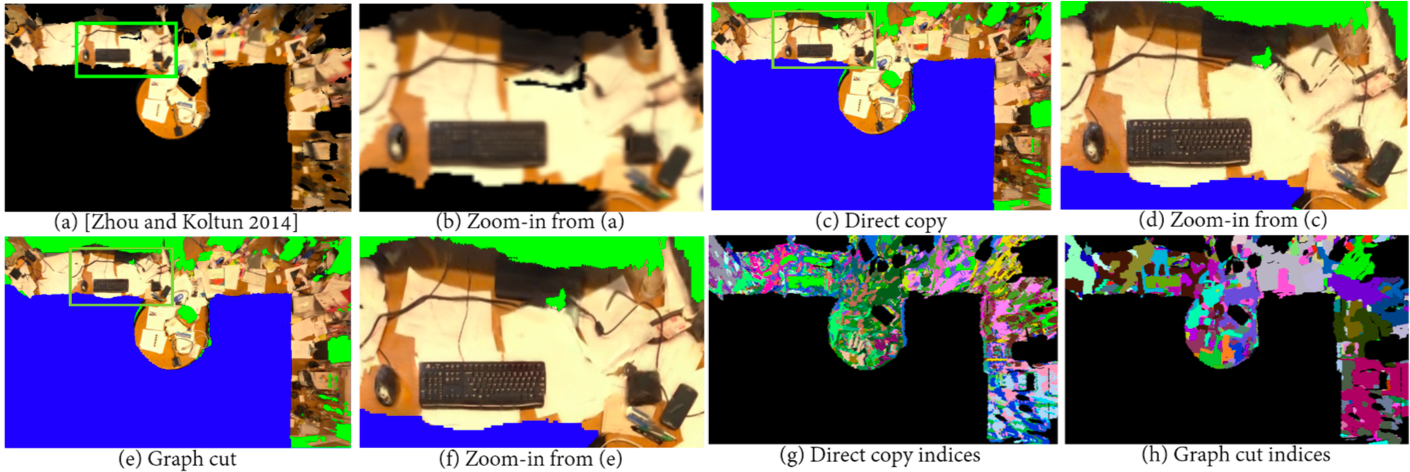
\includegraphics[width=\linewidth]{3dlite/fig5.png}
\caption{Texture generation from multiple frames: (a) Color map optimization~\cite{zhou2014color} (averaging). (b) Zoom-in from (a). (c) Direct copy from sharpest region. (d) Zoom-in from (c). (e) Balance sharpness and region coherence. (f) Zoom-in from (e). (g) Frame indices with sharpest local region. (h) Optimized frame indices for color sampling.
}
\label{fig:3dlite-sharp-graph-cut}
\end{figure}

Figure~\ref{fig:3dlite-sharp-graph-cut} shows a challenging example, where a table texture is composed of projections from the 147 sharpest color frames of more than 3000 images.
We see that directly sampling from frames with the highest region sharpness value ((c),(d)) improves upon the texture sharpness of Zhou and Koltun~\cite{zhou2014color} ((a),(b)), but contains some noise due to lack of coherence in the frames being sampled from. Our final texture sharpening result ((e), (f)) balances both sharpness and frame coherence, preserving sharpness while reducing noise.

Using direct color sampling can still result in noticeable artifacts when transitioning from sampling from one frame to another, as shown in Fig.~\ref{fig:3dlite-sharp-poisson}(b).
We perform a final step in to mitigate these effects in the sharpening process.
We combine the divergence map $\triangle C(p)$ from the labeling resulting from solving Eq.~\ref{eq:3dlite-sharp-graph-cut}, which represents texture information~\cite{perez2003poisson}, with the color map $\bar{C}(p)$ computed by averaging, and solve for the final texture $F(p)$ in the least squares optimization
\begin{equation}
E(F) = \sum_p ||F(p) - \bar{C}(p)||^2 + \lambda ||\triangle F(p) - \triangle C(p)||^2\,.
\label{eq:sharp-poisson}
\end{equation}
As shown in Fig.~\ref{fig:3dlite-sharp-poisson}, this maintains sharpness while removing boundary inconsistencies.

\begin{figure}
\centering
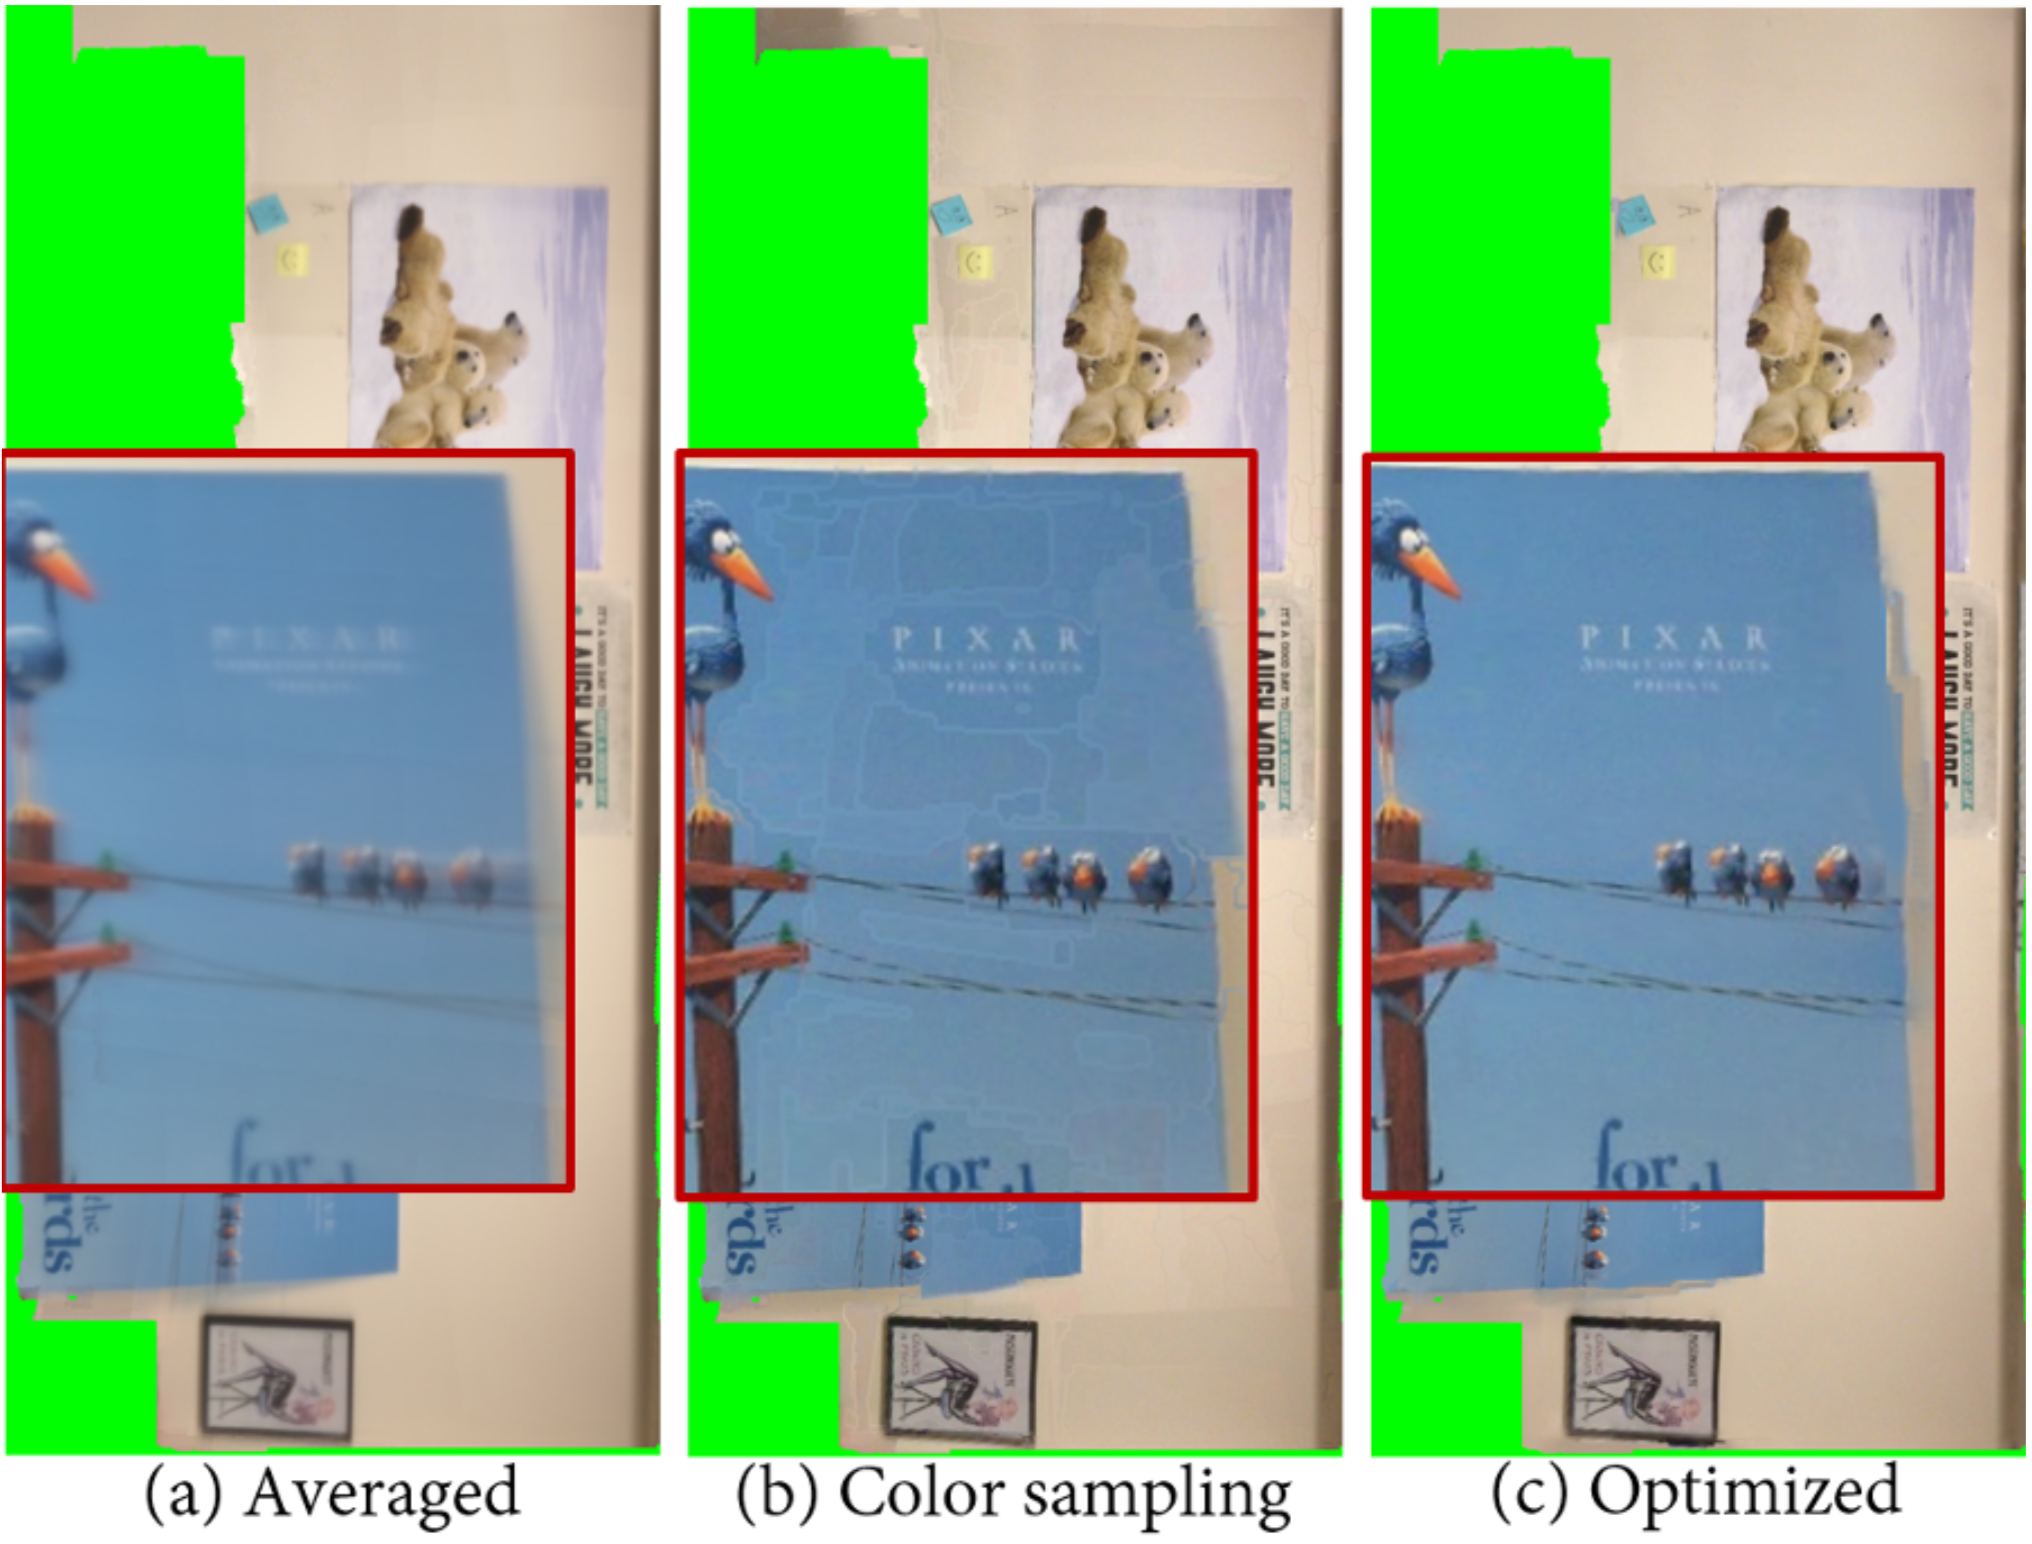
\includegraphics[width=0.8\linewidth]{3dlite/fig6.png}
\caption{Texture optimization combining averaged color and sampled divergence map. (a) Averaged color from all selected frames. (b) Direct color sampling from optimized frame indices. (c) Optimization combining averaged color and sampled divergence map.}
\label{fig:3dlite-sharp-poisson}
\end{figure}

\subsection{Scene completion}
\label{sec:completion}

While our texture-optimized, lightweight mesh contains sharp, compelling color, it nonetheless remains incomplete, due to occlusions or limited scanning coverage.
3D completion is a challenging task, as it typically requires example-based learning techniques~\cite{dai2017complete}, and the problem becomes cubically more complex with  higher resolutions and larger spatial extents.
We thus exploit our planar primitive abstraction to simplify 3D scene completion in both geometry and color.%, as it can be extrapolated to 
\begin{figure}
	\centering
    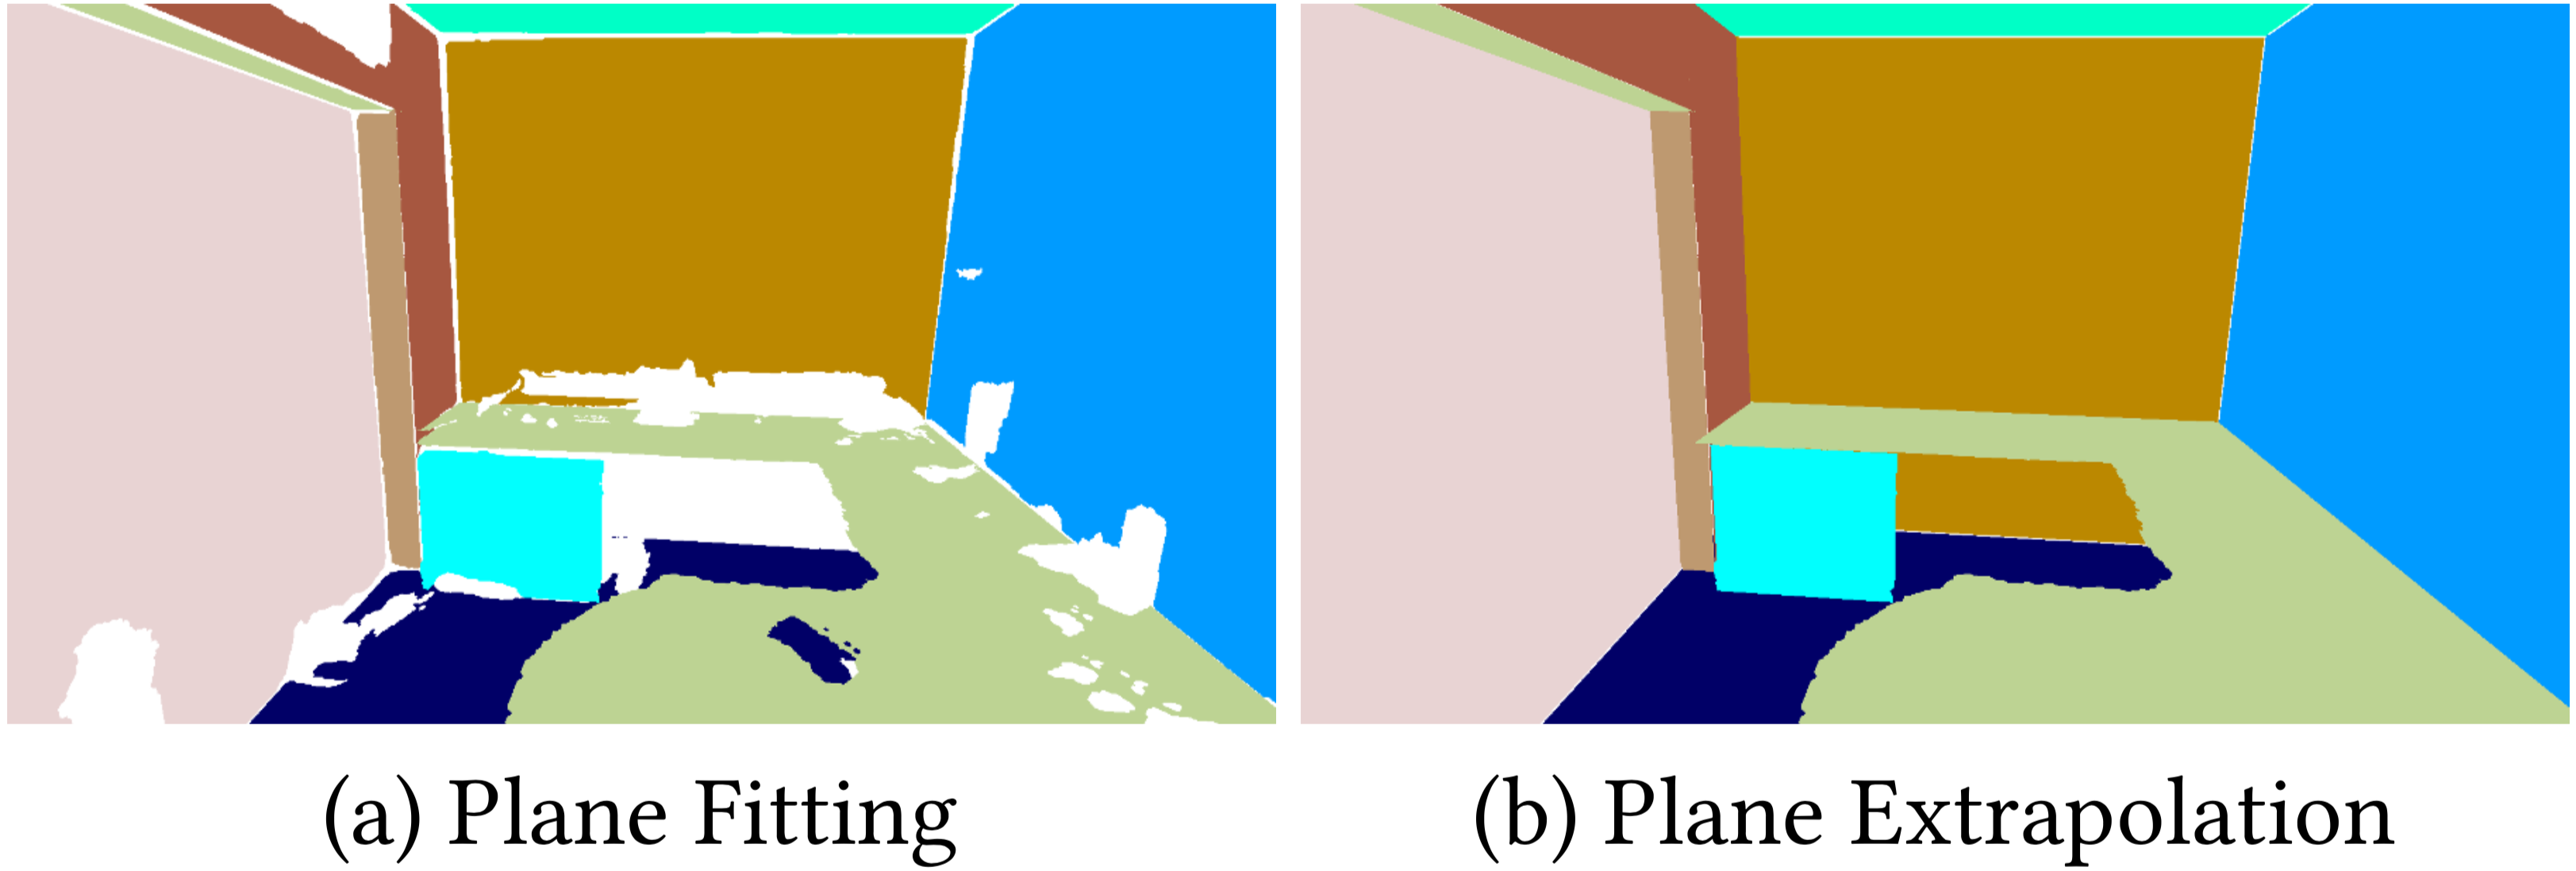
\includegraphics[width=0.8\linewidth]{3dlite/fig7.png}
	\caption{Primitive fitting and extrapolation: (a) After primitive fitting and structural refinement, we project vertices to the primitives, producing a clean mesh. (b) We extrapolate primitives in occluded regions to close the surface.}
	\label{fig:3dlite-plane-fit}
\end{figure}

\subsubsection{Geometry Completion}
\label{subsec:3dlite-extrapolate}
\begin{figure}
	\centering
	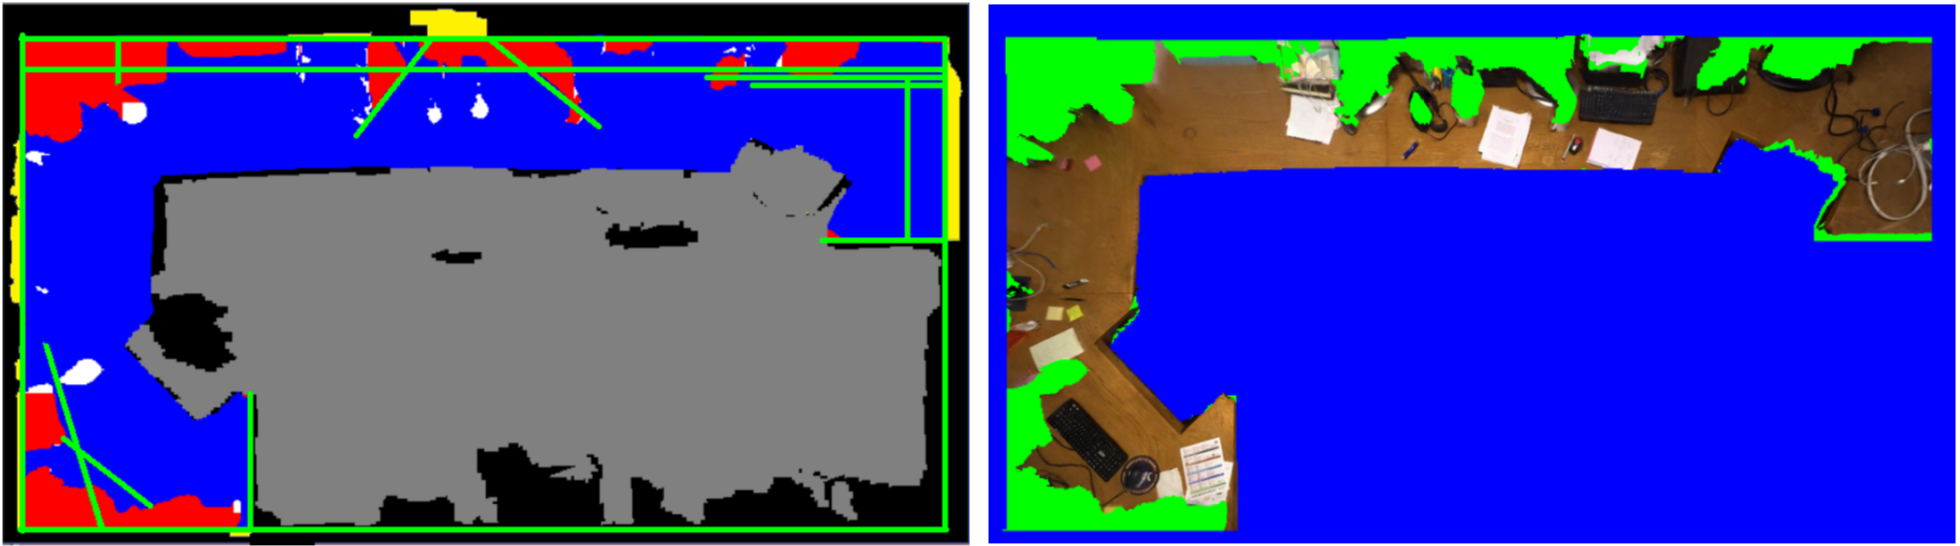
\includegraphics[width=0.8\linewidth]{3dlite/fig9.png}
	\caption{An example of extrapolation and hole filling. Left: Green lines represent possible intersections between sets of planes. Blue represents the original scene geometry, red the extrapolated regions, yellow removed original geometry extending past intersections, gray known empty space, and white self-contained holes which were filled. Right: Completed plane primitive with texture.}
	\label{fig:3dlite-plane-fill}
\end{figure}

A plane-based primitive abstraction enables geometry completion by plane extrapolation in unseen regions~\cite{dzitsiuk2016noising}.
We use several rules to guide our completion approach, visualized in Fig.~\ref{fig:3dlite-extrap-illus}:
\begin{itemize}
	\item Two planes should be extrapolated to their intersection if the extrapolated area is unobserved.
	\item If three planes will intersect each other, extrapolate them to meet at a corner if the extrapolated area is unobserved.
	\item No planes should be extrapolated into open space (observed to be empty). Note that we use the initial TSDF to determine known occupied, known empty, and unobserved space, according to the camera trajectory.
	\item Holes self-contained in a plane should be filled if they are in unobserved space.
\end{itemize}

We search for all pairs of planes satisfying the first rule and extrapolate them. 
Then, we find all triplets of planes under the second rule and extrapolate them. 
Our algorithm is invariant to the extrapolation order since the final state forces all planes to meet in unobserved areas.
For each pair of planar primitives, we attempt to detect potential extrapolation regions, and then repeat the same for all sets of three planar primitives which intersect. Finally, we fill in unobserved holes self-contained within planar primitives.
Note that while this process achieves successful completion for scenes in which parts of all major planes have been observed, we cannot generate geometry from scratch in the case of very large regions of unobserved scene geometry (see Sec~\ref{subsec:3dlite-limitations} for further discussion).

Figs.~\ref{fig:3dlite-plane-fit} and \ref{fig:3dlite-plane-fill} demonstrate our extrapolation and hole-filling to generate complete scenes.

\begin{figure}
	\centering
	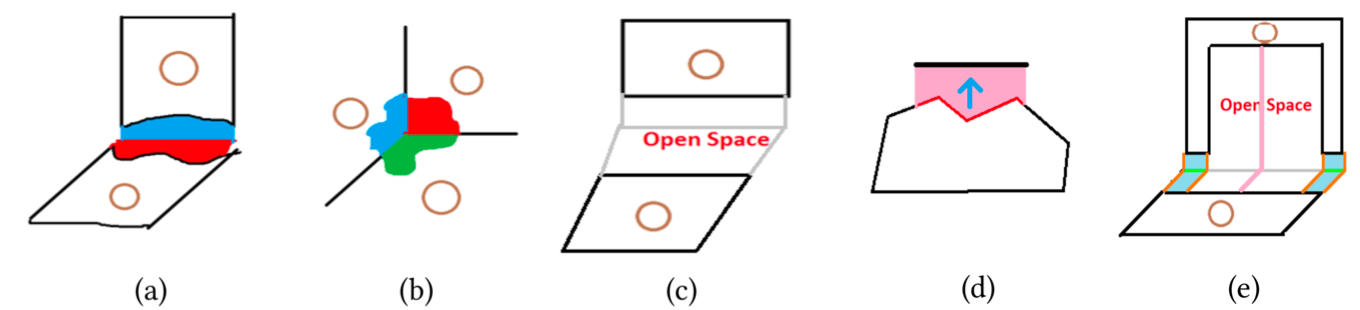
\includegraphics[width=0.8\linewidth]{3dlite/fig8.png}
	\caption{Rules for plane extrapolation. (a) Two planes should extrapolate to their intersection. (b) Three planes should extrapolate to their intersection. (c) No planes should be extrapolated through known empty space. (d) Extrapolation (light red) can be viewed as a certain boundary (red) extending in the direction (blue) orthogonal to the intersection line. (e) A more complex example, showing invalidation of potential extrapolation due to known empty space. Only the blue regions should be extended towards the intersection.}
	\label{fig:3dlite-extrap-illus}
\end{figure}

\subsection{Texture Completion}
\label{subsec:3dlite-inpaint}
Our plane-based primitive abstraction reduces the 3D texture completion problem into a two-dimensional one over plane textures.
As this texture synthesis problem is a classical one and has been well-studied~\cite{criminisi2004region,simakov2008summarizing,barnes2009patchmatch,darabi2012image,wang2016unsupervised,pathak2016context,yang2016high}, we employ state-of-the-art image inpainting techniques to complete texture in geometry-extrapolated regions.

Although recent deep learning based methods have shown impressive results, they require a large training set and are mostly constrained to fixed image resolutions. 
Thus we use Image Melding~\cite{darabi2012image}, a patch-based approach incorporating image transforms and gradients into a mixed $\ell_2/\ell_0$ optimization to achieve high-quality image inpainting.
We found the method to work well for most cases, except when there are incomplete regions of a texture which cover a distinct foreground and smooth background, or when there are shadows on the background, as shown in Fig.~\ref{fig:3dlite-synthesize}(b).
In these cases, we detect the background using image segmentation~\cite{felzenszwalb2004efficient}, and extend it to fill the entire image using laplacian smoothing (Fig.~\ref{fig:3dlite-synthesize}(c)).
We then combine the synthesized background with the foreground (Fig.~\ref{fig:3dlite-synthesize}(d)), and synthesize pixels less than $10$ pixels from the foreground using Image Melding (Fig.~\ref{fig:3dlite-synthesize}(e)).

\begin{figure}
	\centering
    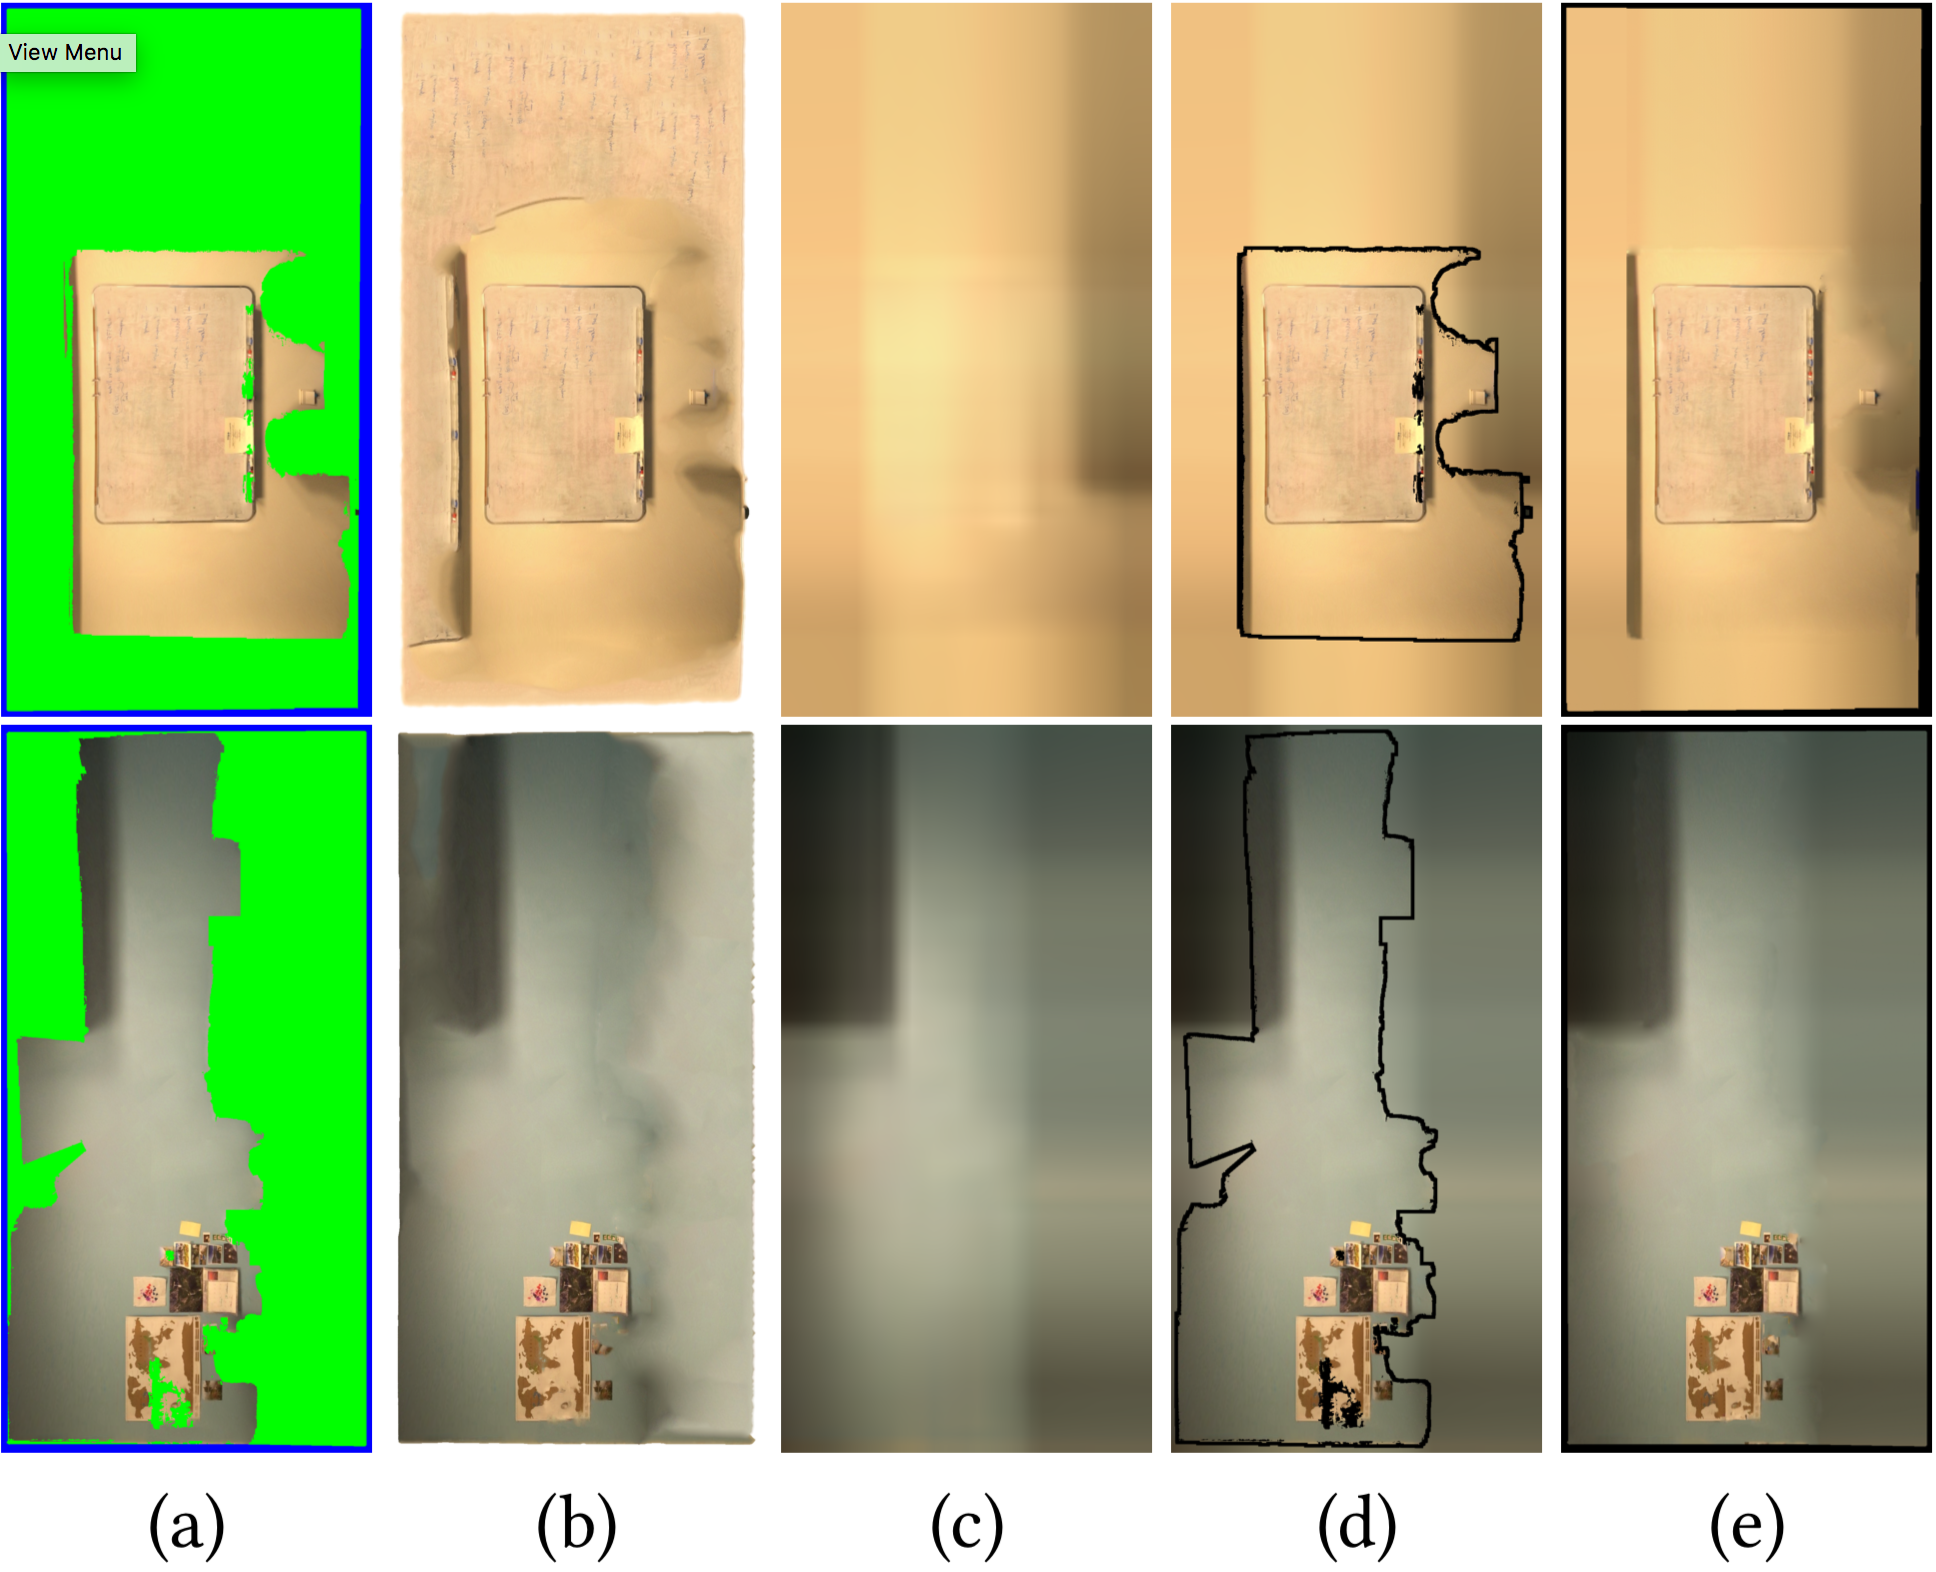
\includegraphics[width=0.8\linewidth]{3dlite/fig10.png}
	\caption{Texture completion. (a) Original texture with green denoting regions to be synthesized. (b) Direct application of Image Melding~\cite{darabi2012image}. (c) Background color estimation. (d) Combined background and original texture. (e) Remaining pixels inpainted with Image Melding.}
	\label{fig:3dlite-synthesize}
\end{figure}

\subsection{Mesh Generation}
\label{sec:approach-mesh}
In section, we discuss the procedure to generate the final light-weight mesh. 
We first denoise plane boundaries and then convert the planar primitive abstraction to a mesh, producing a final model $\approx 25$ times smaller than the original mesh.

\paragraph*{Boundary Refinement.}
Plane boundaries are often noisy, due to noise and distortion in the input sensor data and the initial reconstruction.
To denoise the boundaries, we smooth them with a combination of line and B-spline fitting.
Lines are fit to each vertex on the boundary (sampled at every 8mm) by using its $51$ neighboring vertices. 
A vertex belongs to a line if the condition number of the covariance of these vertices is larger than 50.
We then iteratively merge line-associated neighbor vertices together if their lines are no more than $5^\circ$ apart.
We fit B-splines to each consecutive sequence of vertices not belonging to any lines.

\begin{figure}
\centering
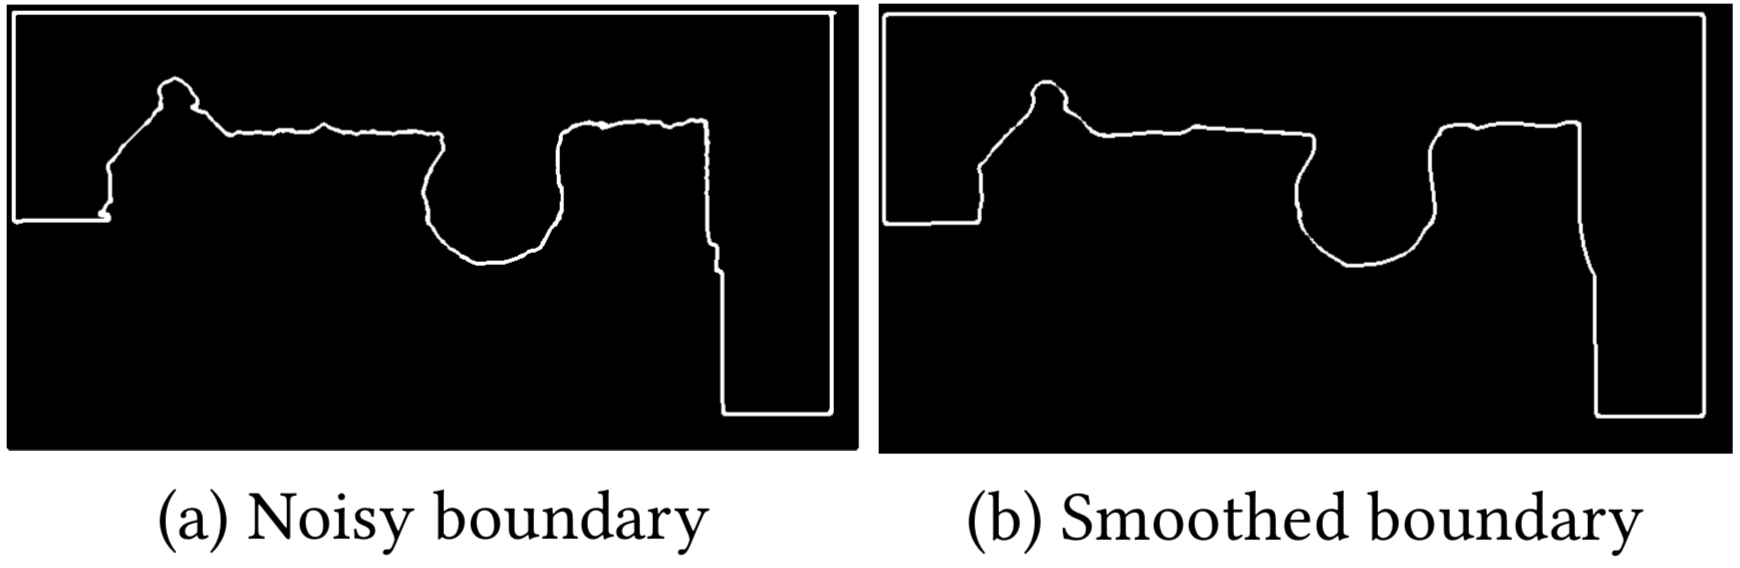
\includegraphics[width=0.8\linewidth]{3dlite/fig11.png}
\caption{Smoothing the boundary. Initial plane primitive boundaries are noisy (left), which we smooth with B-Splines and lines (right).}
\label{fig:boundary-fit}
\end{figure}

\paragraph*{Primitive Remeshing.}
To generate our final mesh, we triangulate the planar primitives using constrained Delaunay triangulation~\cite{chew1987constrained}. 
Figure~\ref{fig:3dlite-remesh}(a) shows the resulting simplified triangle mesh, which accurately preserves primitive boundaries.
Because we use discretized pixels to generate the original primitive boundaries, there can be small gaps between primitives which should be connected. 
To close these gaps, we project vertices near primitive intersections to the intersecting primitive, as shown in Figure~\ref{fig:3dlite-remesh}(b).
\begin{figure}
\centering
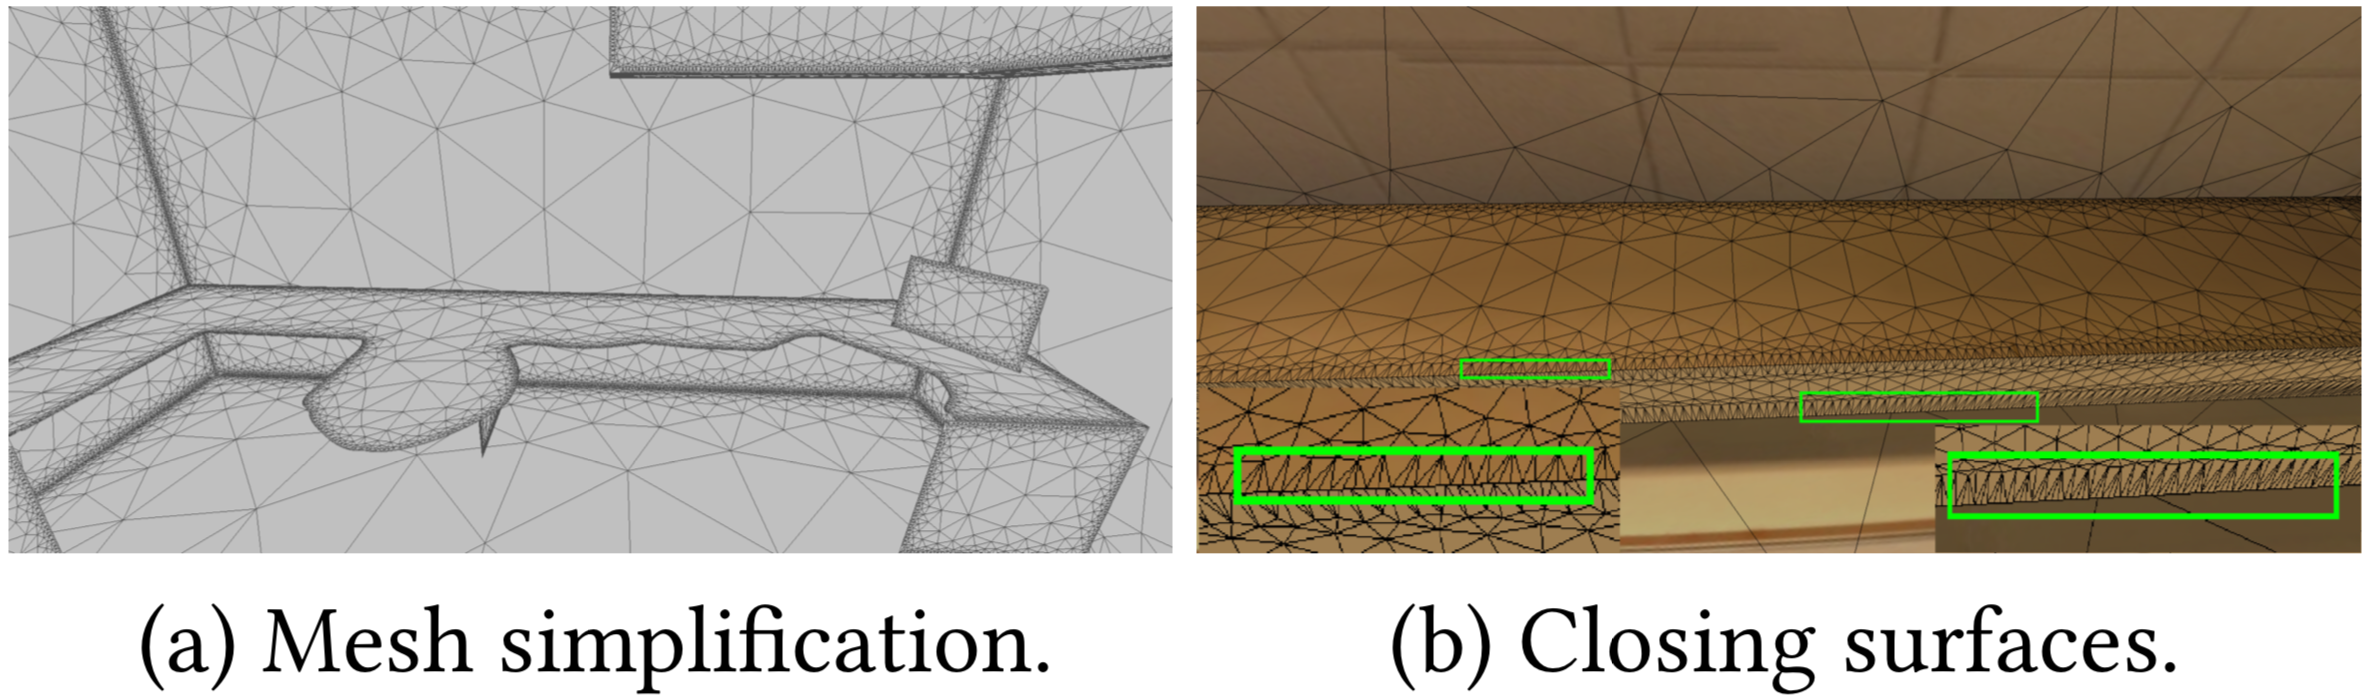
\includegraphics[width=0.8\linewidth]{3dlite/fig12.png}
\caption{Mesh simplification and vertex projection. (a) We simplify the planar primitives with constrained Delaunay triangulation. (b) We apply vertex projection to close the surfaces which should be connected.}
\label{fig:3dlite-remesh}
\end{figure}


\subsection{Results}
\label{sec:results}

We tested our method on a variety of RGB-D scans of indoor scenes.
All scans were captured using a \emph{Structure Sensor}\footnote{https://structure.io} mounted to an iPad Air, including several sequences from the BundleFusion data~\cite{dai2016bundlefusion} as well as the ScanNet~\cite{dai2017scannet} dataset.
We use $640\times 480$ color and depth, synchronized at $30$Hz.
Note that we are agnostic to the type of RGB-D sensor used.
For each scan, we compute the initial camera poses using BundleFusion. 
All 3DLite experiments  were performed on an Intel Core i7 2.6GHz CPU, with each scan taking on average 5 hours to process.
Detailed timings are shown in Table~\ref{table:3dlite-timing}.
\begin{table}
\center
\begin{tabular}{|c|c|c|c|c|c|}
\hline
& \multicolumn{3}{|c|}{BundleFusion Scenes} & \multicolumn{2}{|c|}{ScanNet}\\
\hline
Scenes & office0 & office1 & office3 & 0567\_01 & 0451\_05\\
\hline
Region(s) & 478 & 503 & 531 & 472 & 523\\
\hline
Plane(s) & 21.5 & 17.1 & 23.2 & 16.5 & 25.4\\
\hline
Sharpness(s) & 1138 & 1186 & 1266 & 811 & 8436\\
\hline
Color(s) & 11458 & 9553 & 14432 & 9866 & 9315\\
\hline
Boundary(s) & 1.156 & 1.101 & 1.157 & 0.781 & 1.384\\
\hline
\hline
& \multicolumn{3}{|c|}{ScanNet} & \multicolumn{2}{|c|}{other}\\
\hline
Scenes & 0294\_02 & 0271\_01 & 0220\_02 & apt & offices \\
\hline
Region(s) & 535 & 511 & 517 & 585 & 897\\
\hline
Plane(s) & 23.9 & 18.7 & 27.4 & 38.1 & 61.8\\
\hline
Sharpness(s) & 1011 & 828 & 935.4 & 1151 & 1968\\
\hline
Color(s) & 16407 & 9601 & 8575 & 18226 & 35976\\
\hline
Boundary(s) & 1.219 & 0.921 & 1.406 & 2.016 & 3.725\\
\hline
\end{tabular}
\caption{Timings (seconds) for different components.
}
\label{table:3dlite-timing}
\end{table}

\emph{Qualitative comparison.}
We first compare our lightweight, textured meshes of 10 scenes with 3D reconstructions computed using BundleFusion and VoxelHashing~\cite{niessner2013real}.
Note that since BundleFusion's online re-integration updates use color discretized to bytes, there may be some small color artifacts in the resulting reconstruction, so we first run BundleFusion to obtain camera poses and then compute a surface reconstruction with VoxelHashing.
As shown in Figs.~\ref{fig:3dlite-result-model} and \ref{fig:3dlite-result-tex}, even with simplified geometry, our high quality textures provide visually compelling results on completed scenes, drastically reducing various color oversmoothing artifacts.

\begin{figure}[!htb]
   \begin{minipage}{0.49\textwidth}
     \centering
	\includegraphics[width=\linewidth]{3dlite/fig13.png}
	\caption{Reconstructed meshes with high-quality surface textures. 
		3DLite produces completed scenes while significantly reducing color artifacts compared to reconstructions generated with BundleFusion~\cite{dai2016bundlefusion} and VoxelHashing~\cite{niessner2013real}.
	}
	\label{fig:3dlite-result-model}
   \end{minipage}\hfill
   \begin{minipage}{0.49\textwidth}
	\includegraphics[width=\linewidth]{3dlite/fig14.png}
	\caption{Zoomed-in views showing our reconstructed 3d models compared to reconstructions produced by BundleFusion~\cite{dai2016bundlefusion} and VoxelHashing~\cite{niessner2013real}.}
	\label{fig:3dlite-result-tex}
   \end{minipage}
\end{figure}


\emph{Primitive abstraction.}
We show several examples of our primitive-based geometry in Fig.~\ref{fig:3dlite-eval-plane}, which allows us to produce denoised and complete geometry compared to the original reconstruction, in a much more lightweight representation, which is more than 300 times smaller than the original mesh under the same resolution. The face number of our scenes is shown in Table~\ref{table:3dlite-face-num}.
\begin{table}
\center
\begin{tabular}{|c|c|c|c|c|c|}
\hline
& \multicolumn{3}{|c|}{BundleFusion Scenes} & \multicolumn{2}{|c|}{ScanNet}\\
\hline
Scenes & office0 & office1 & office3 & 0567\_01 & 0451\_05\\
\hline
FaceNum & 62559 & 68874 & 63479 & 43153 & 89621\\
\hline
\hline
& \multicolumn{3}{|c|}{ScanNet} & \multicolumn{2}{|c|}{other}\\
\hline
Scenes & 0294\_02 & 0271\_01 & 0220\_02 & apt & offices \\
\hline
FaceNum & 58709 & 58790 & 82864 & 92898 & 174200 \\
\hline
\end{tabular}
\caption{Number of faces in 3DLite models.
}
\label{table:3dlite-face-num}
\end{table}

\begin{figure}
\begin{minipage}{0.49\linewidth}
\centering
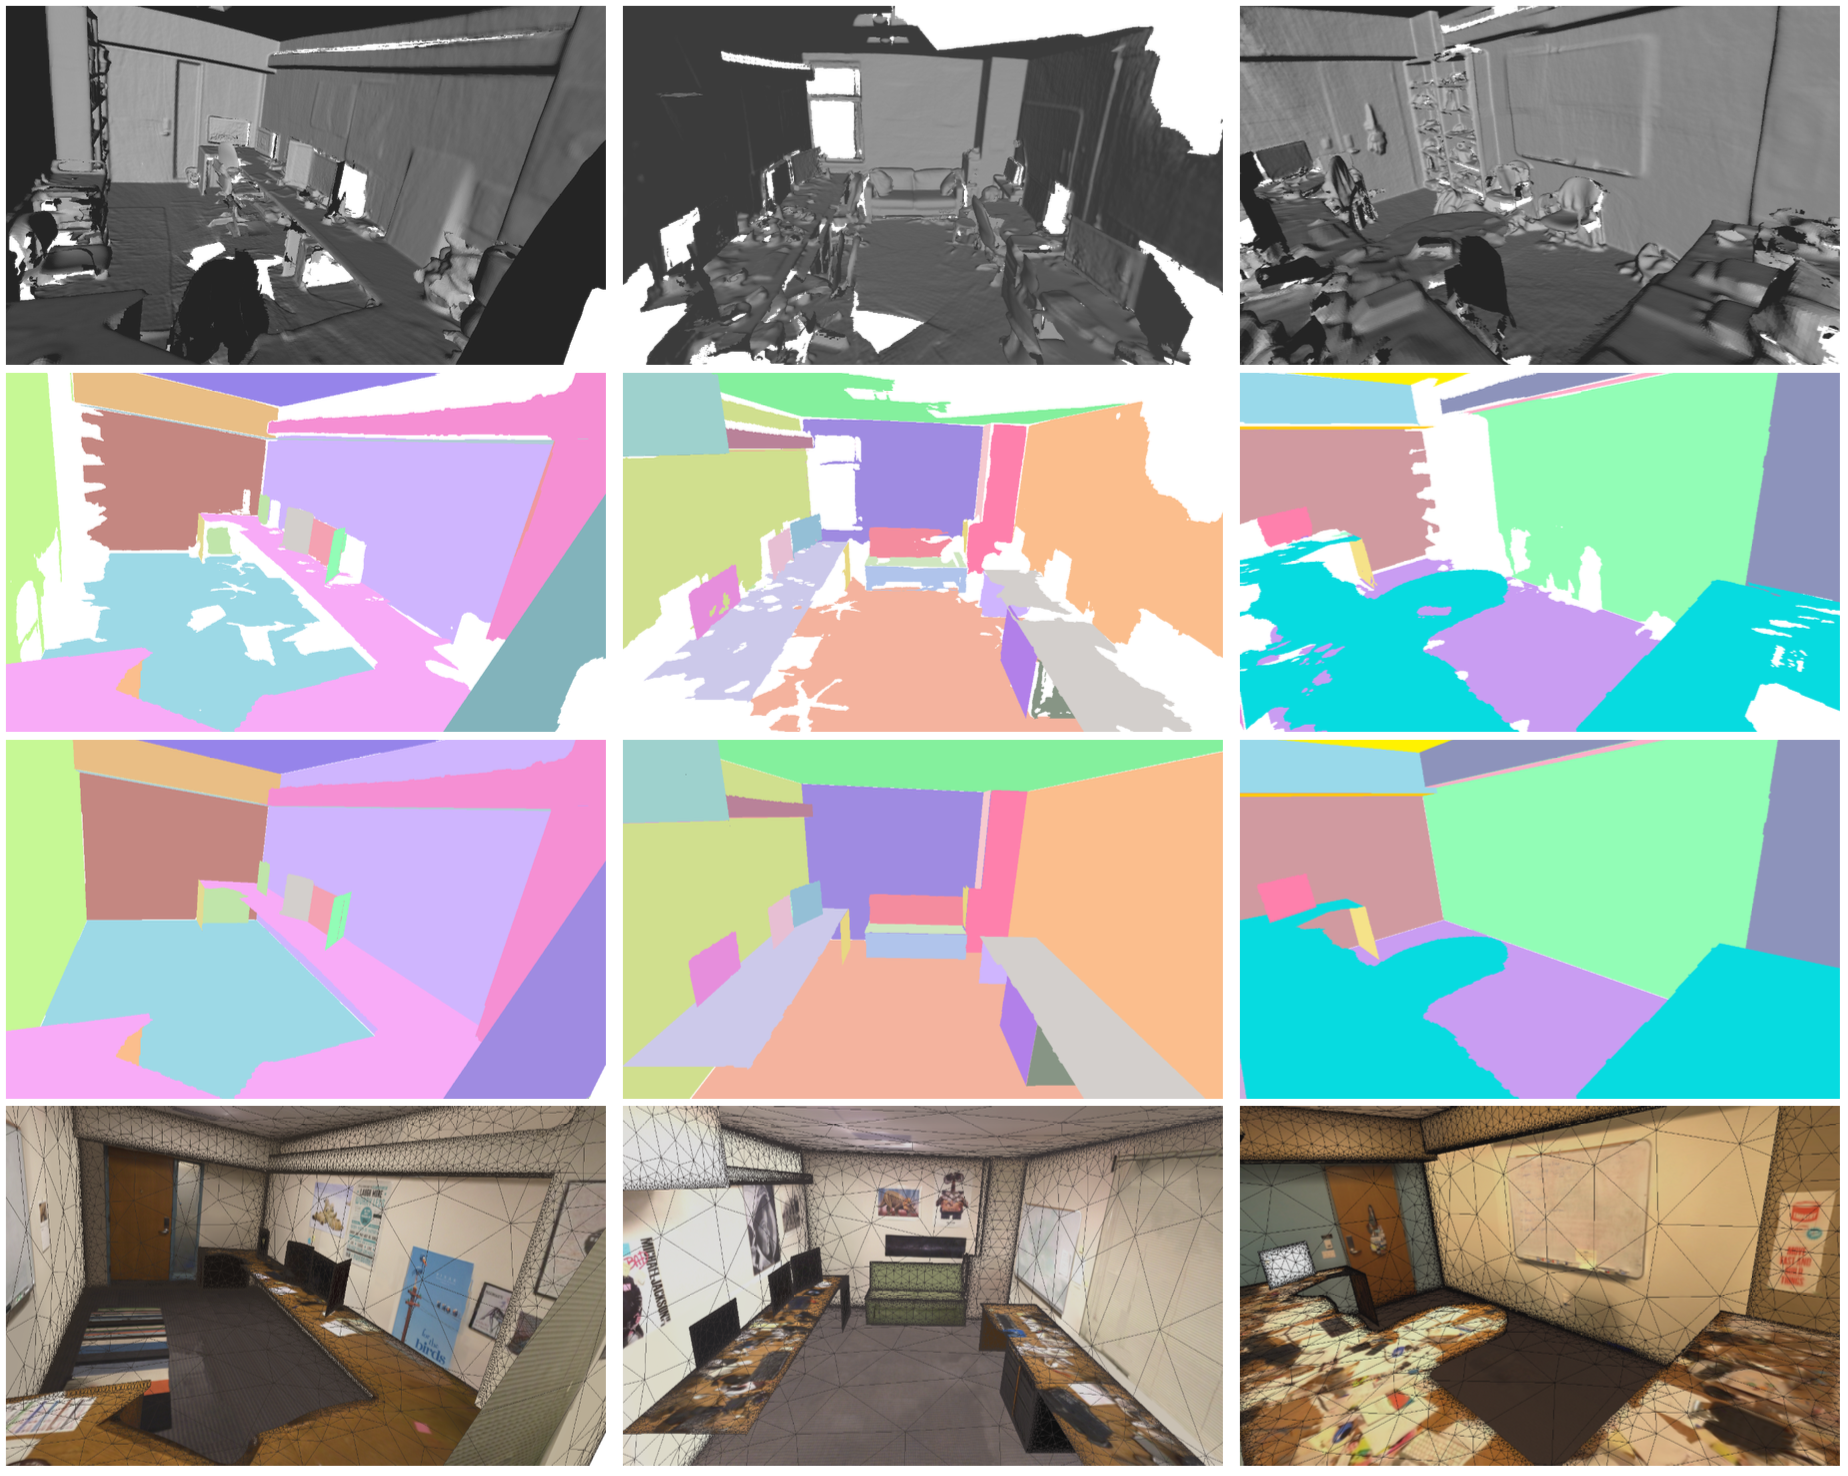
\includegraphics[width=\linewidth]{3dlite/fig15.png}
\caption{Primitive-based Abstraction. First row: original mesh. Second row: after primitive fitting. Third row: after geometry completion by primitive extrapolation. Last row: final result after texture mapping and mesh generation.}
\label{fig:3dlite-eval-plane}
\end{minipage}
\begin{minipage}{0.49\linewidth}
\centering
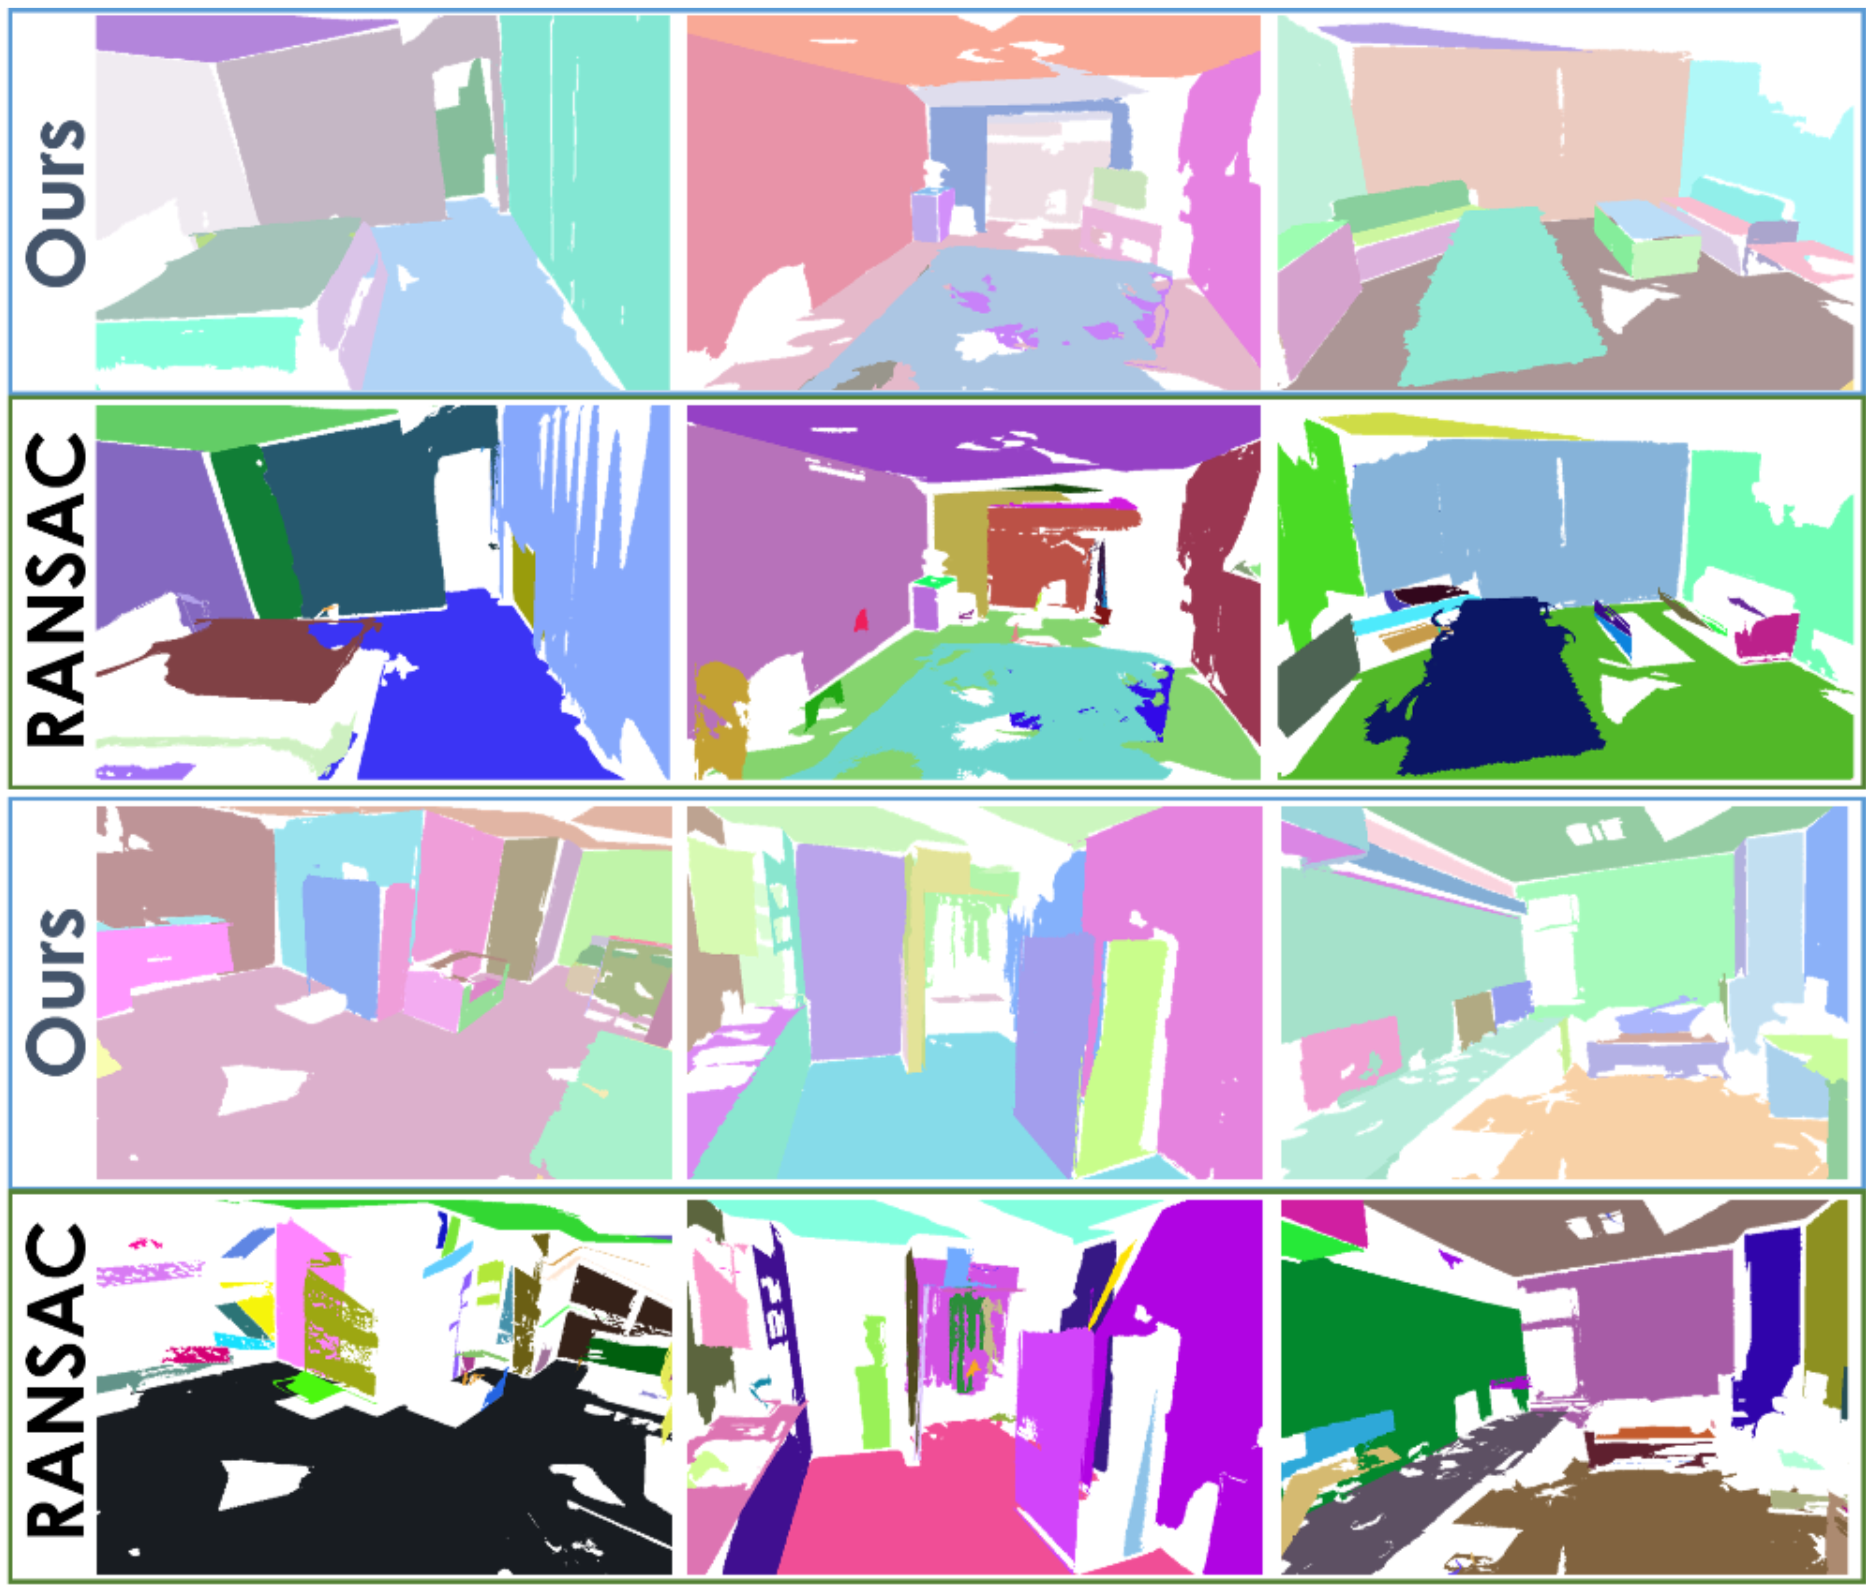
\includegraphics[width=\linewidth]{3dlite/fig16.png}
\caption{Comparison between our method and plane fitting with RANSAC.  Our method is more robust in detecting relatively small planes.}
\label{fig:3dlite-eval-fitting}
\end{minipage}
\end{figure}

Compared to traditional plane fitting using RANSAC, our method is more robust in detecting relatively small planes, as shown in Fig.~\ref{fig:3dlite-eval-fitting}.

\emph{Color alignment.}
We analyze our color alignment approach, showing the effect of our sparse and primitive geometry terms in Fig.~\ref{fig:3dlite-eval-align-rigid} (optimizing for rigid poses only).
Without color optimization, the result contains oversmoothing and ghosting. 
Optimizing for rigid poses under a dense photometric error using Zhou and Koltun~\cite{zhou2014color} sharpens the image but still retains some artifacts where initial camera poses were too far from the basin of convergence.
Our new terms are able to bring the optimization to a precise alignment of color frames.

\begin{figure}
\begin{minipage}{0.49\linewidth}
\centering
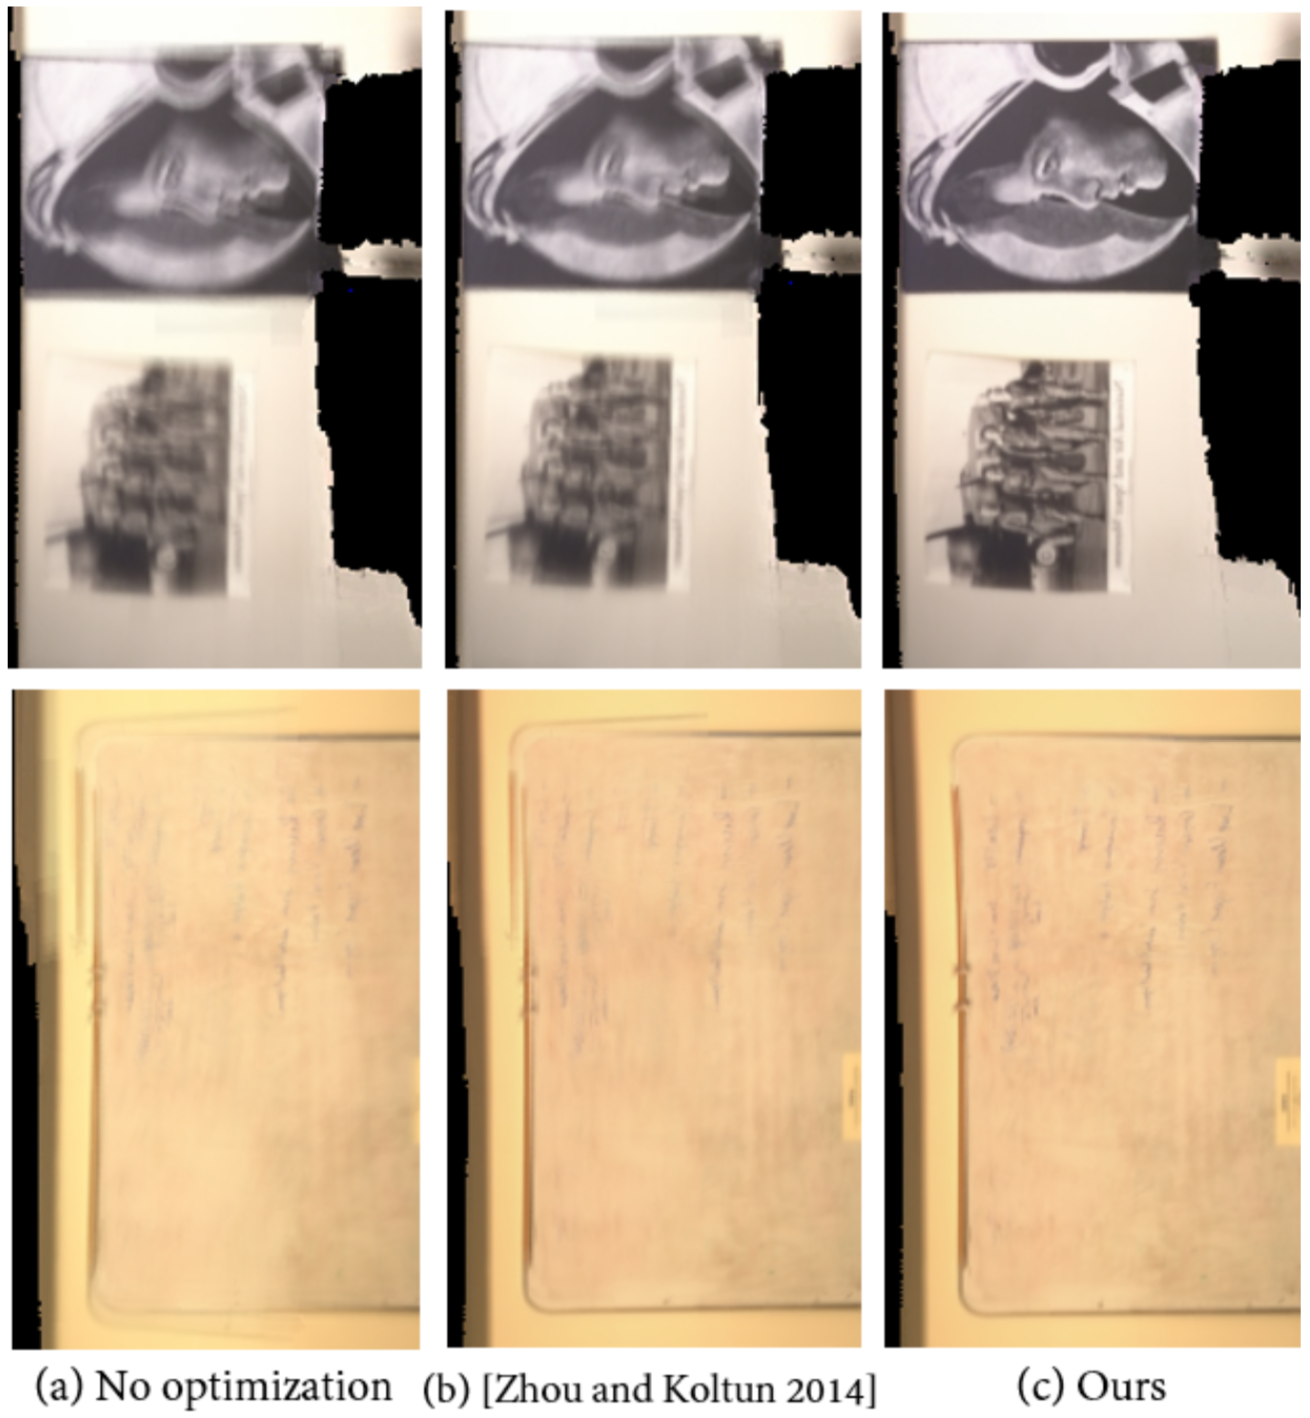
\includegraphics[width=\linewidth]{3dlite/fig17.png}
\caption{Color Alignment. (a) Color averaging. (b) Camera poses optimized with only dense color~\cite{zhou2014color}. (c) Camera poses optimized using our method, with dense color, sparse feature and geometry information.}
\label{fig:3dlite-eval-align-rigid}
\end{minipage}
\begin{minipage}{0.49\linewidth}
\centering
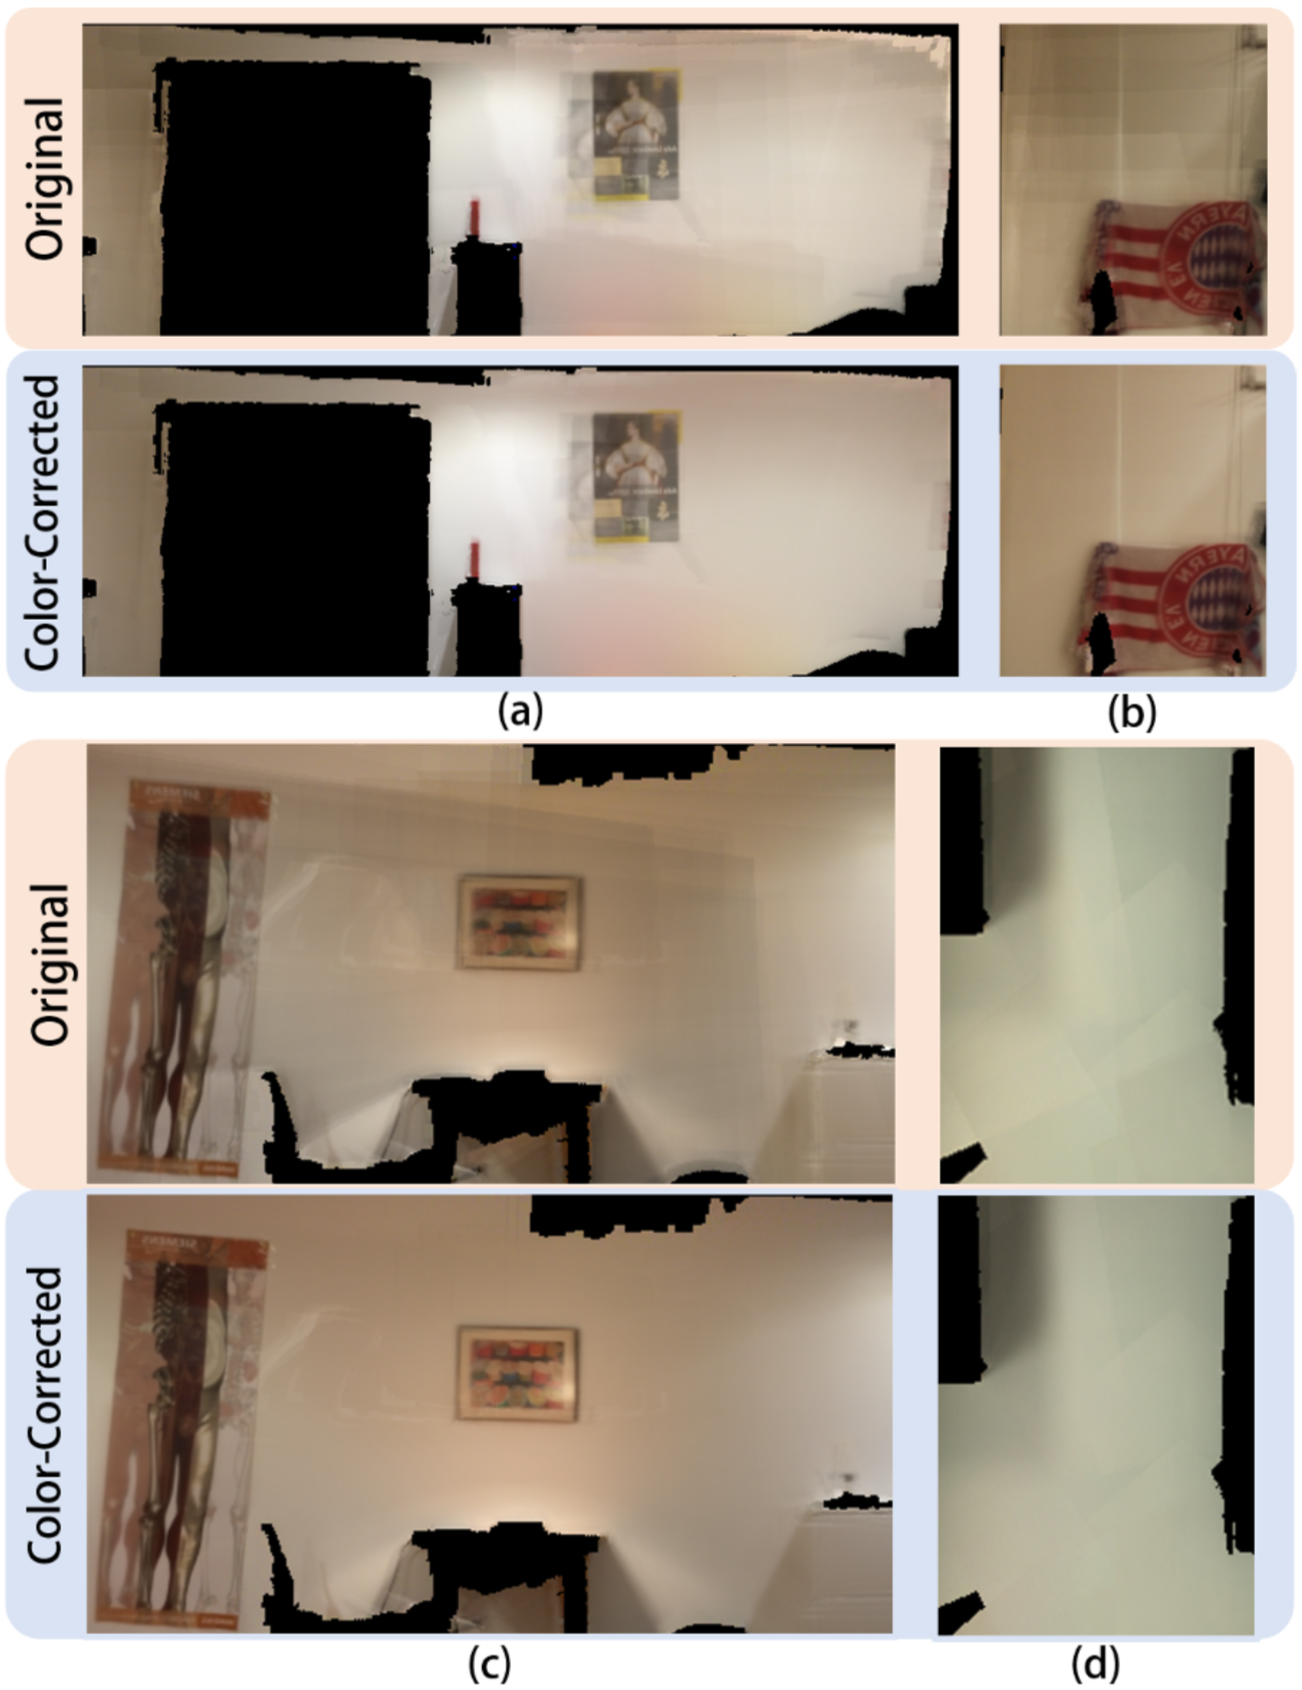
\includegraphics[width=0.8\linewidth]{3dlite/fig18.png}
\caption{Color transfer correction. (a)(b), and (d) are taken with auto exposure and white balancing, and (c) with fixed exposure and white balancing. Our color transfer optimization compensates for color inconsistencies in both scenarios. }
\label{fig:3dlite-eval-color-transfer}
\end{minipage}
\end{figure}

\begin{figure}
\begin{minipage}{0.49\linewidth}
\centering
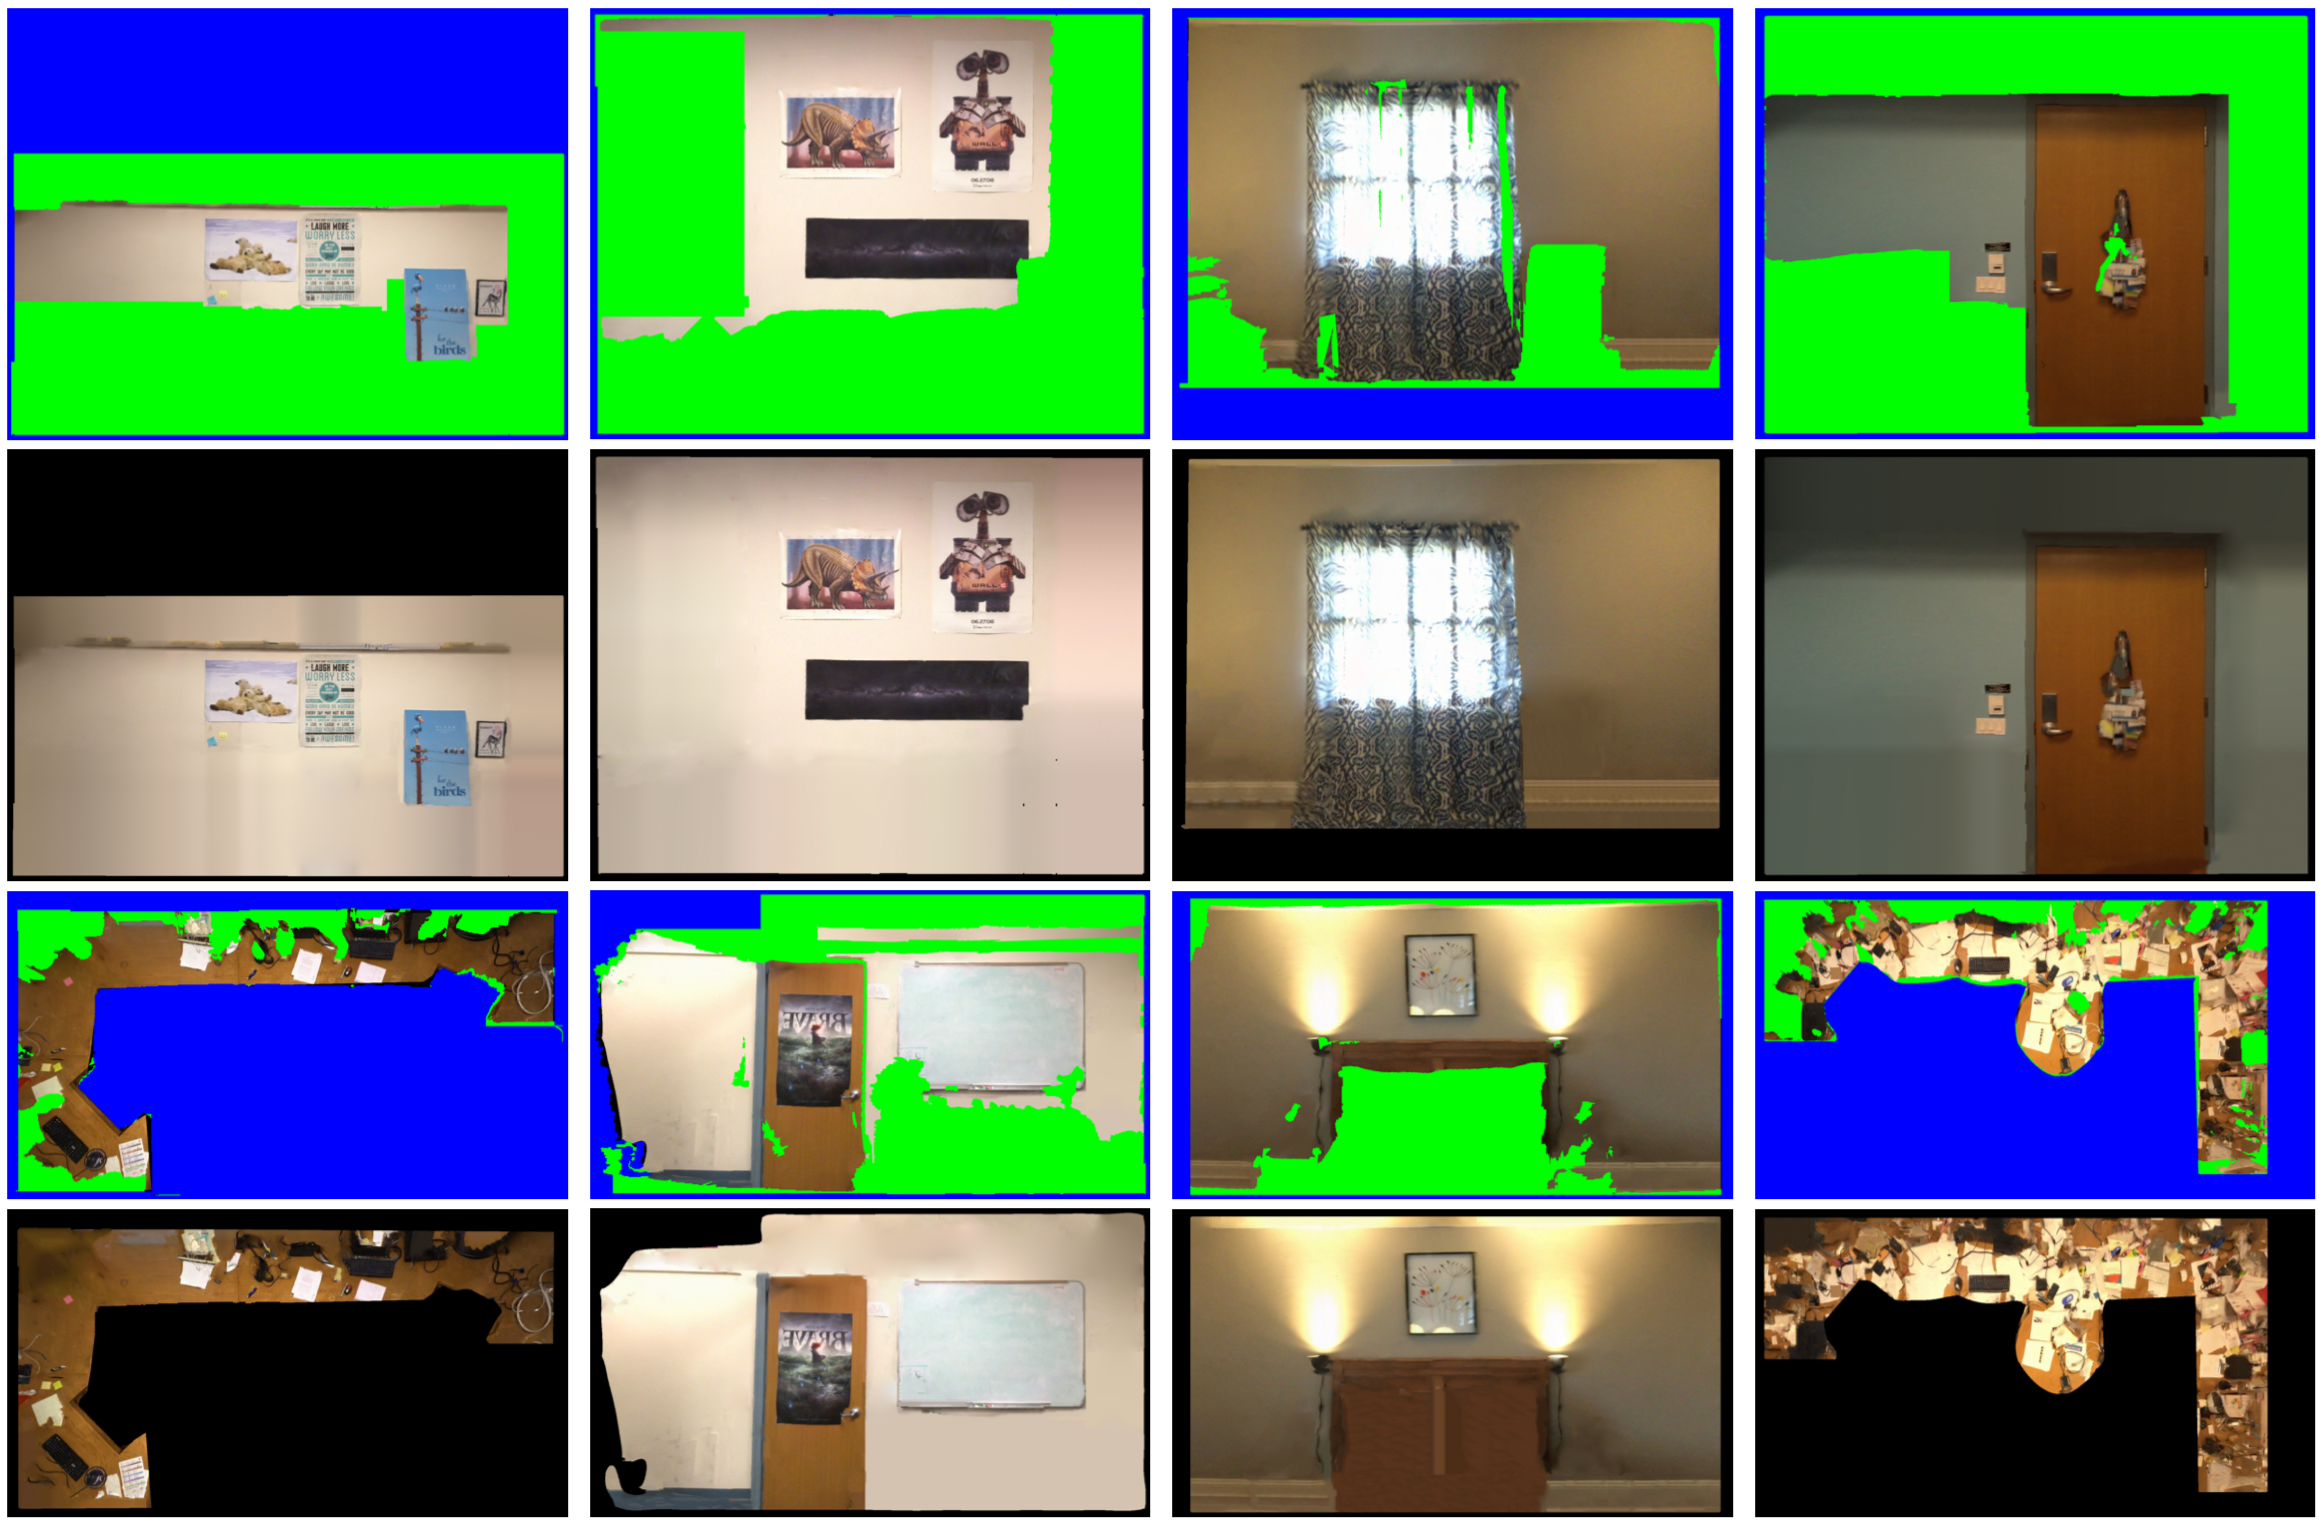
\includegraphics[width=\linewidth]{3dlite/fig20.png}
\caption{Texture completion using background filling with Image Melding~\cite{darabi2012image} to synthesize missing colors. Green represents unobserved regions to be synthesized, and blue empty space.}
\label{fig:3dlite-eval-complete}
\end{minipage}
\begin{minipage}{0.49\linewidth}
	\centering
    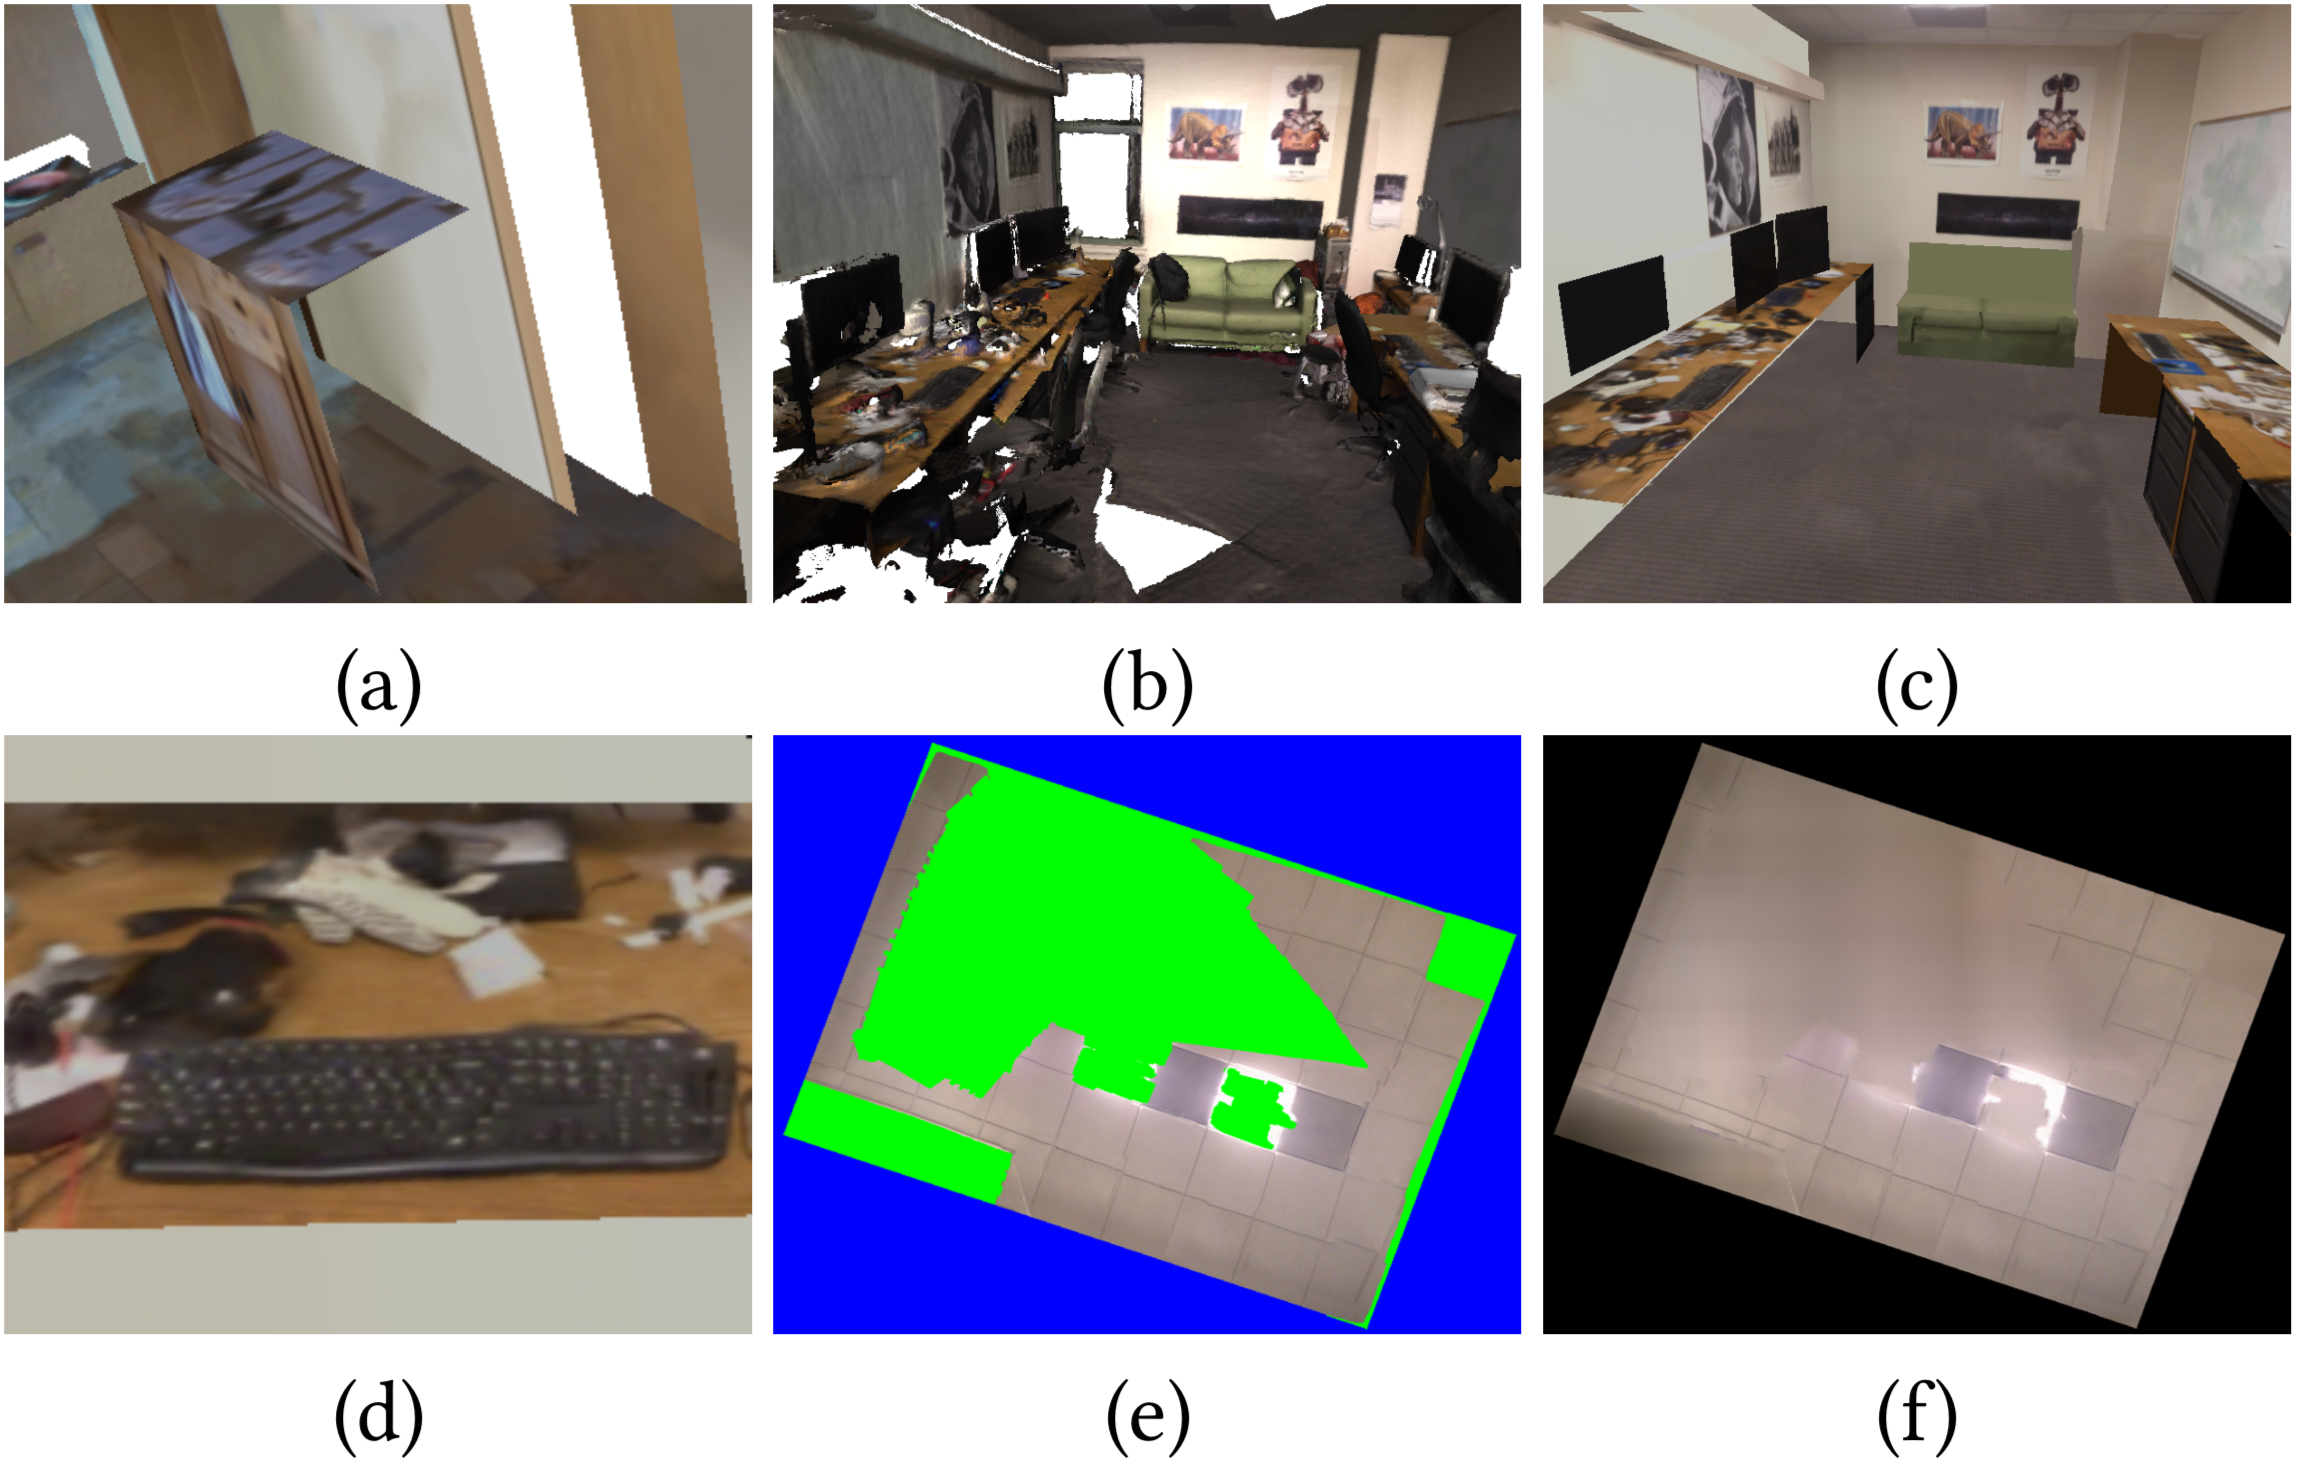
\includegraphics[width=\linewidth]{3dlite/fig21.png}
\caption{Limitations of our method. (a) Geometry entirely unseen in the original scan cannot be synthesized. (b-c) Non-planar objects (e.g., some chairs) are not captured by our current primitive abstraction. (d) Small objects may be projected onto planar surfaces, as the depth camera resolution is low. (e-f) Texture inpainting can have difficulty synthesizing large missing regions.}
	\label{fig:3dlite-limitation}
\end{minipage}
\end{figure}

\begin{figure}
\centering
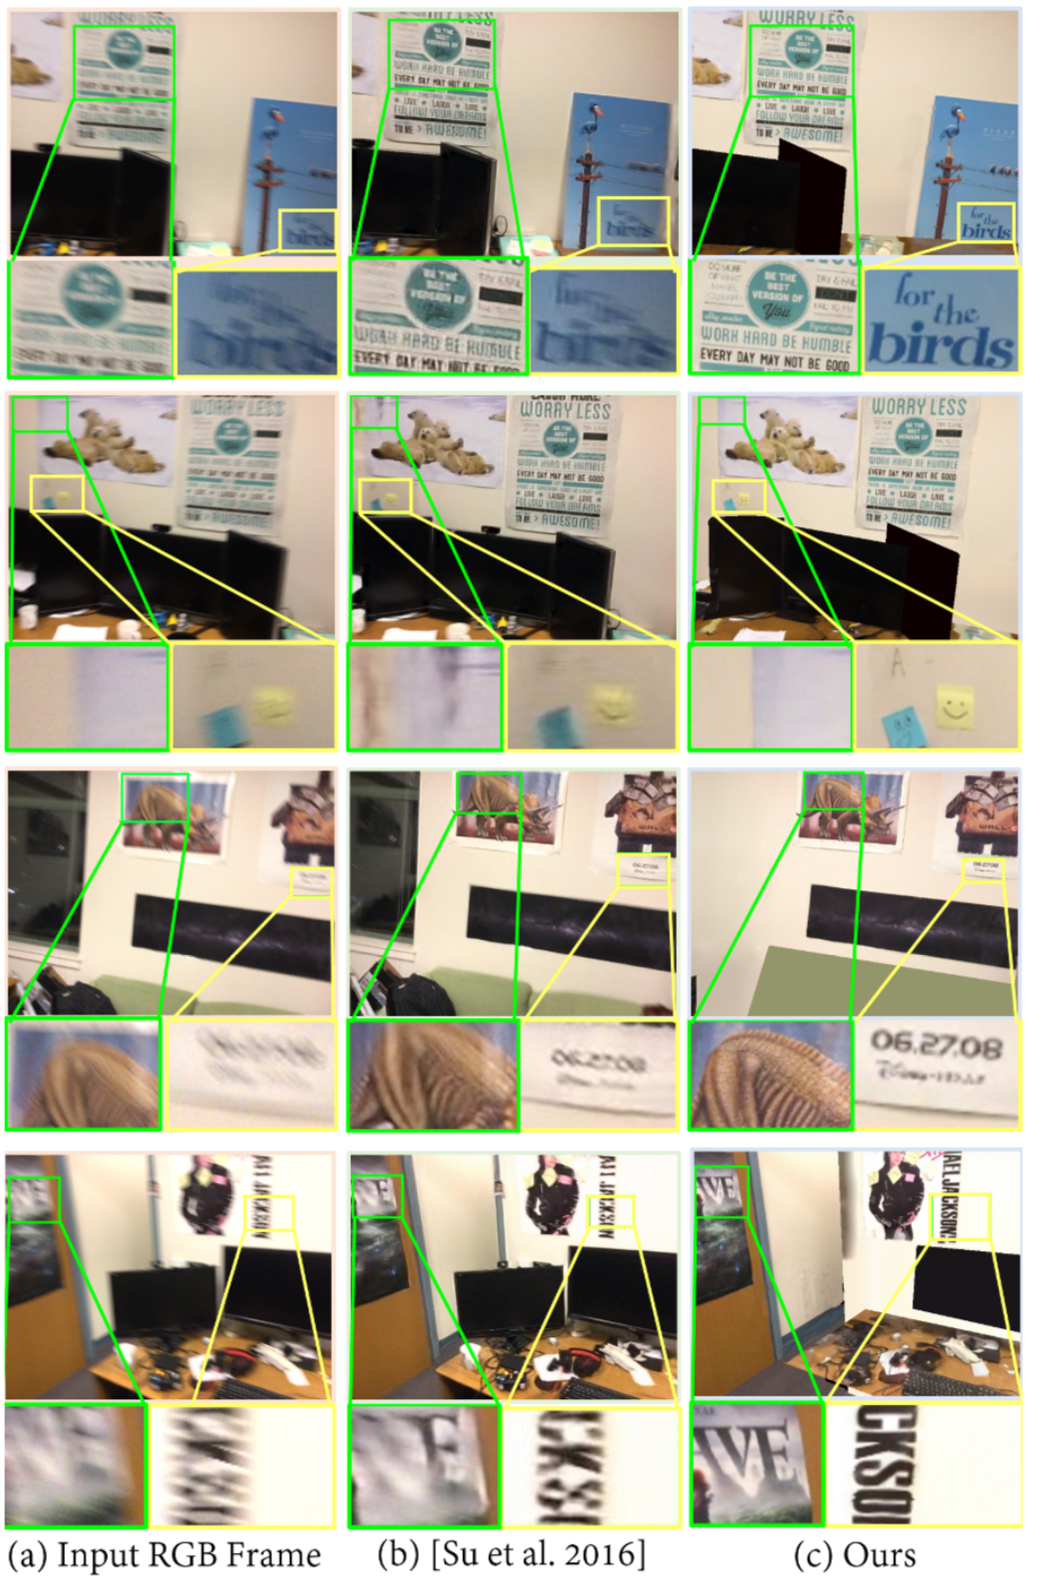
\includegraphics[width=\linewidth,height=1.2\linewidth]{3dlite/fig19.png}
\caption{Texture sharpening comparison. (a) Most input RGB frames are blurry. (b) Deep Video Deblurring~\cite{su2016deep} reduces some of the blur. (c) Our approach produces consistently sharp results.}
\label{fig:3dlite-eval-deblur}
\end{figure}

\emph{Color transfer correction.}
We show the effect of the color transfer optimization in Fig.~\ref{fig:3dlite-eval-color-transfer}, significantly reducing not only visible artifacts from auto-exposure and auto-white balancing, but also various color inconsistencies which can occur even under fixed exposure and white balancing settings.

\emph{Texture sharpening.}
In Fig.~\ref{fig:3dlite-eval-deblur}, we show the effectiveness of our texture sharpening approach.
Since we generate a consistent texturing from sharp regions of the input images, images rendered from our 3D model can be sharper than some of the original RGB images (which often contain motion blur), as well as deblurred RGB images using advanced video motion deblur techniques~\cite{su2016deep}.
Such deblurring, while noticeably reducing blur in several parts of the image, still has some difficulty near image boundaries, and with large motion.

\emph{Texture completion.}
Fig.~\ref{fig:3dlite-eval-complete} shows several texture completion results using background filling along with Image Melding~\cite{darabi2012image} to synthesize colors in unobserved regions.
We are thus able to generate complete scene models with textured geometry.

\subsection{Limitations}
\label{subsec:3dlite-limitations}

While 3DLite can robustly generate lightweight, abstracted models with sharp textures, it still suffers from several limitations, as visualized in Fig.~\ref{fig:3dlite-limitation}.
If there is geometry entirely unseen in the original scan, we cannot generate it from scratch to complete these regions. 
Additionally, small objects (e.g., keyboards, mice) are often projected onto planar primitives; this is not too dissimilar from reconstructions generated from volumetric fusion, where the coarse resolution, noise, and distortion of a commodity depth sensor can also make small objects difficult to distinguish geometrically.
Further, while state-of-the-art texture synthesis methods can achieve impressive results, they are not perfect, and may still have difficulty synthesizing color in large missing regions.
Most notably, our current primitive abstraction is plane-based, so relatively non-planar objects (e.g., some chairs) are not captured in our geometric abstraction. We hope to extend our approach in combination with CAD model retrieval, alignment, and texturing in order to retain all scene geometry and texture.

\section{Adversarial Texture}
\label{sec:tadv}
\subsection{Method}

\begin{figure*}
    \centering
    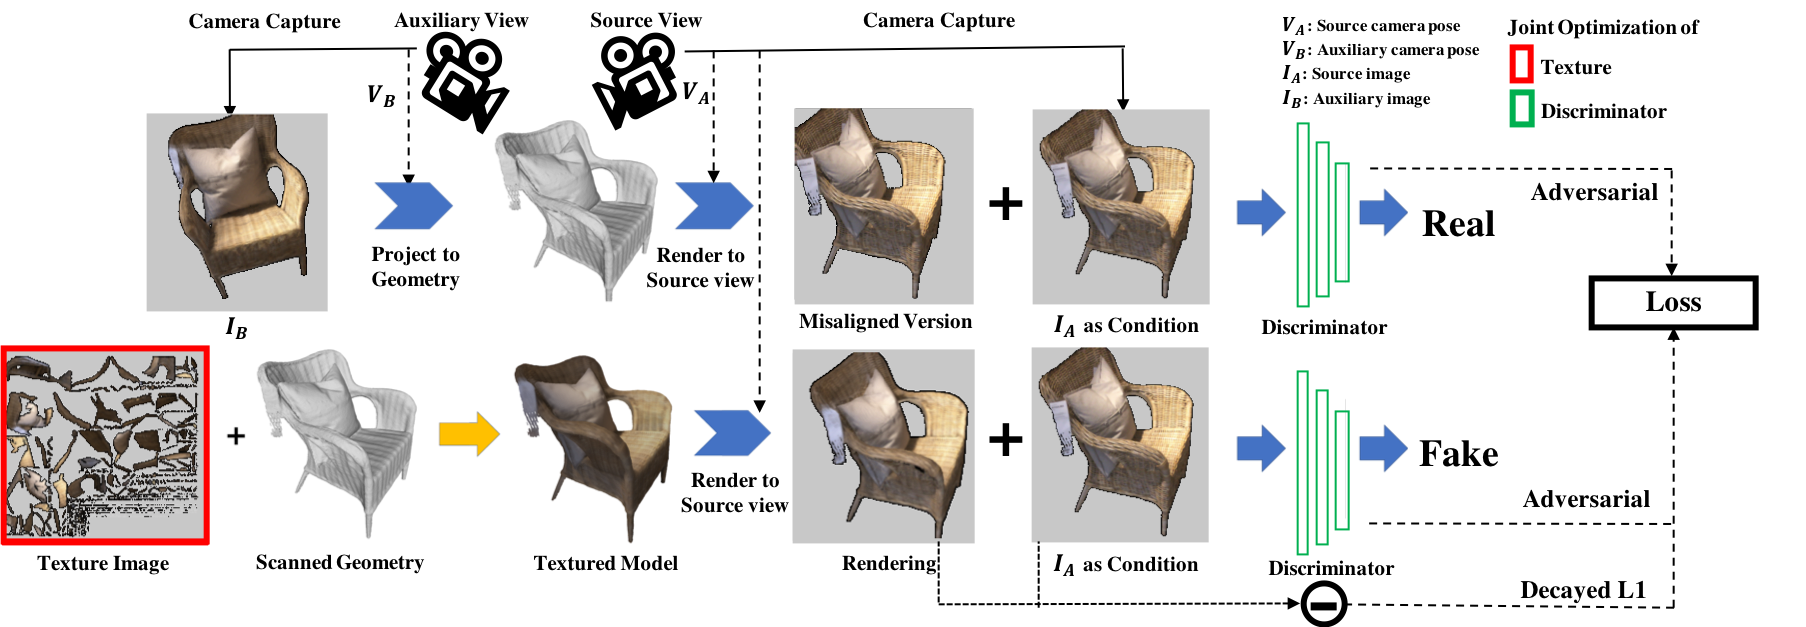
\includegraphics[width=\linewidth]{texturegen/figures/pipeline.png}
    \caption{Texture Generation. 
    From an input RGB-D scan, we optimize for both its texture image and a learned texture objective function characterized by  a discriminator network. 
    The discriminator operates on reprojections of input color images in order to maintain robustness to various misalignments.
    We randomly pick a pair of input images, \emph{source} and \emph{auxiliary}, and synthesize the fake and real examples from the source view, conditioned on the re-projected source image. 
    The texture image and discriminator are trained in an alternating process.}
    \label{fig:toptim-pipeline}
\end{figure*}

Our goal is the optimization of a color texture that can be used to render a scanned scene using a classical computer graphics pipeline.
%
During the scanning procedure, we obtain color images and their estimated camera poses.
%
These views, along with the reconstructed geometry, are input to our method.
%
To optimize for a color texture, we must specify an objective function; in this case, we need to account for misalignments of the color images and the reconstructed model.
%
To this end, we propose to learn the loss function in conjunction with the texture (see Figure~\ref{fig:toptim-pipeline}).
%
The function is modeled as an adversarial loss using a discriminator network identifying `real' and `fake' imagery, and is designed to provide a misalignment-tolerant metric for our texture optimization.
%

\subsection{Misalignment-Tolerant Metric}
\label{sec:approach-misalign}



%
Our key insight is to propose to learn a conditional discriminator as a misalignment-tolerant metric adaptive to the error distribution of the input data.
%
Figure~\ref{fig:toptim-misalign-example}(a) shows a 2D example where two observations (b) and (c) are misaligned by 2 units in the horizontal directions, and an L2 loss results in blurry appearance.
%
Ultimately, we aim to synthesize a texture that appears as realistic as either observation.
%
To achieve this, we ask the discriminator to consider both (b) and (c) as real conditioned on either observation.
%
With such a discriminator, the blurred (d) results in a large loss and the texture will instead converge to either (b) or (c).
%

%
We extend this intuition to 3D where the geometry is observed from different viewpoints.
%
We then aim to optimize a texture such that local patches of the texture rendered to various views look realistic.
%
Therefore, conditioned on any arbitrary view, we generate real examples by a re-projection from any other view to this view, as shown in Figure~\ref{fig:toptim-pipeline}.
%
Such re-projection can be achieved by projecting the color image onto the surface and then rendering back to another view.
%
Unlike the simple 2D example, it is highly possible that there is no texture solution so that each local patch perfectly matches the one view from the input images, given camera and geometry error.
%
However, the proposed approach is expected to push those inconsistencies to the smooth textured regions to hide any artifacts that can be easily identified by the discriminator, and thereby producing locally consistent realistic texture solution.
%

%
For each optimization iteration, we randomly select two input images, $I_A$ (source image) and $I_B$ (auxiliary image) with corresponding camera poses $V_A$ and $V_B$.
%
The conditioning is $I_A$ from the viewpoint $V_A$, and the `real' image is $I_B$ projected to the scan geometry and rendered from $V_A$, while the `fake' image is the synthesized texture rendered from $V_A$.
%
We alternating optimize the texture and discriminator.
%
During texture optimization, we adjust the texture pixel colors to maximize the adversarial loss such that it looks more realistic under the discriminator scoring.
%
During discriminator optimization, we minimize the adversarial loss such that it better classifies real and fake examples.
%
We linearly combine adversarial loss with an L1 loss that decays exponentially as the optimization proceeds, which helps the optimizer find a good initial texture solution.
%


\begin{figure}
    \centering
    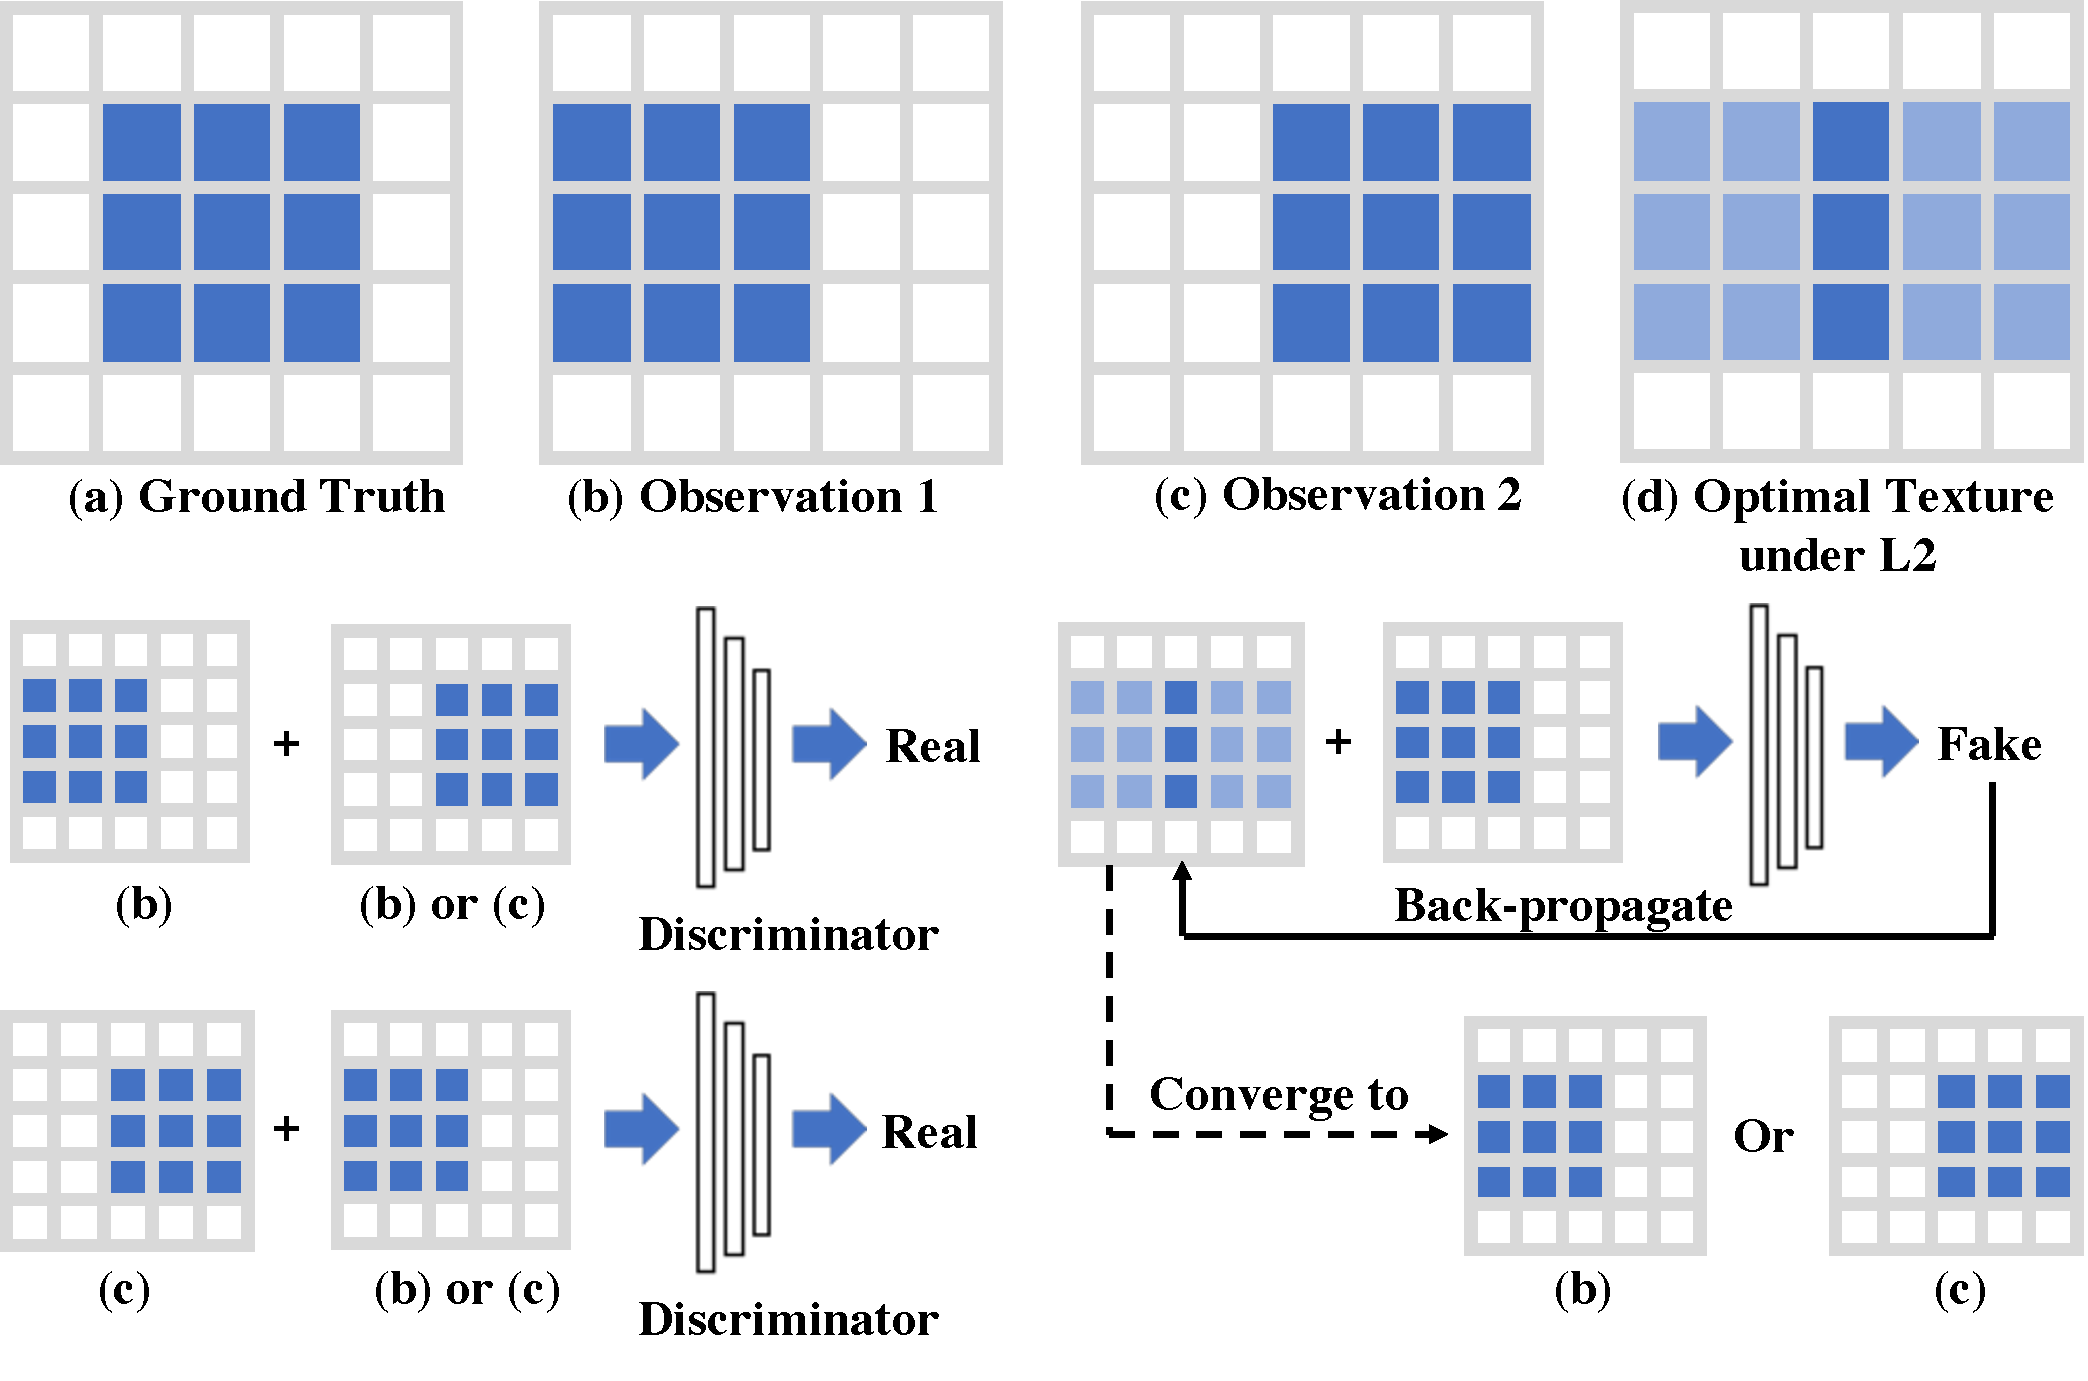
\includegraphics[width=0.75\linewidth]{texturegen/figures/intuitive.pdf}
    \caption{2D example of a misalignment. (a) shows the ground truth pattern, which is observed with misalignment in (b) and (c); an L2 loss results in blurring (d). 
    We train a discriminator which only accepts (b) and (c) as real examples conditioned on each other, and use it to optimize the texture, which converges to either (b) or (c).}
    \label{fig:toptim-misalign-example}
\end{figure}

\paragraph{Network Architecture}
%
Our framework is adopted from the PatchGAN discriminator architecture proposed by Isola et al.~\cite{isola2017image}.  We choose that framework because it is designed to produce local details that look as realistic as a given set of input images.
%
We use three convolutional layers, resulting in a patch size of $70\times 70$, which we find suitable for our input images of resolution $640\times 480$.
%
Unlike the original, we remove all batch normalization layers and feed a single view example for each optimization iteration, which we empirically found to improve performance.
%
Conditioned on the input view, we ask the discriminator to evaluate the residual of the synthesized example subtracted by the condition input.
%
Finally, since we focus on evaluating foreground regions (pixels corresponding to input geometry), we remove the loss terms for regions where background comprises more than $90\%$ of the receptive field.
%

%\subsection{Conditional Adversarial Loss}
\subsection{Texture Optimization}% of the Texture and the Metric}

%
To retrieve a texture, we jointly optimize the texture and the misalignment-tolerant metric.
%The texture and the misalignment-tolerant metric is learned jointly.
%
Inspired by the adversarial loss used in Pix2Pix~\cite{isola2017image}, we express our view-conditioned adversarial loss as:
\begin{align}
\begin{split}
    \mathcal{L}_c(T,D) &= \mathbb{E}_{x,y}(\log D(x,y)) +\\ &\mathbb{E}_{x,M_x}(\log (1 - D(x, M_x(T) ) ),
\end{split}
\end{align}
where $T$ and $D$ represent the target texture image and the discriminator parameters we are optimizing for.
%
$x$ is the condition, a reprojected color image from the input sequence of captured images.
%
$M_x$ is the fixed texture-to-image mapping given the camera pose associated with $x$. 
%
Here, a real example is an image $y$ re-projected to the view of $x$.
%
We optimize $D$ with the objective to correctly identify real examples, misaligned real imagery, and fake examples rendered from the texture as $M_x(T)$. 
%
Simultaneously, we optimize the texture $T$ such that it is difficult to be identified as fake when mapped to view of $x$.
%

%
Since the adversarial loss alone can be difficult to train, we additionally add an L1 loss to the texture optimization to provide initial guidance for the optimization:
%
\begin{equation}
\mathcal{L}_{L1}(T) = \mathbb{E}_{x,y,M_x} ||y - M_x(T)||_1.
\end{equation}
Our objective texture solution is:
\begin{equation}
    T^* = \arg \min_{T} \max_{D} \mathcal{L}_c(T,D) + \lambda \mathcal{L}_{L1}(T).
\end{equation}

%
During training, we initialize all pixels in texture image to zero and $\lambda=10$.
%
The high $\lambda$ allows the L1 loss to provide an initial texture, and for every 1000 steps we exponentially decay the lambda by a factor of $0.8$.
%
We optimize in alternating fashion for each optimization step, using the Adam optimizer for both the texture and discriminator with learning rates $10^{-3}$ and $10^{-4}$ respectively.
%
For each object or scene, we optimize for 50000 steps to finalize our texture. 
%

\subsection{Differentiable Rendering and Projection}
%
%In the fake example synthesis, we need to render the texture into the view together with the gradient information.
To enable the optimization of the RGB texture of a 3D model, we leverage a differentiable rendering to generate synthesized `fake' views.
We pre-compute a view-to-texture mapping, and can then implement the rendering with a differentiable bilinear sampling layer. 

To create the misaligned `real' images ($I_B$ seen from $V_A$), we compute a reprojection; note that here we do not need to maintain gradient information.
For each pixel $\mathbf{P}_A$ in the source image, we need to determine the corresponding pixel $\mathbf{P}_B$ in the auxiliary image, so that a bilinear sampling can be applied to warp image from the $V_B$ to $V_A$. 
Specifically, for $\mathbf{P}_A$ with depth value $d_A$ from the source depth map, we can determine its 3D location in the source view's space as $\mathbf{p_A}=d_A\mathbf{K}^{-1}\mathbf{P_A}$ where $\mathbf{K}$ is the intrinsic camera matrix. 
Suppose the transformations from the camera to the world space for the source and the auxiliary views are given as $\mathbf{T}_A$ and $\mathbf{T}_B$, the corresponding 3D and pixel location in the auxiliary view are $\mathbf{p}_B=\mathbf{T}_B^{-1}\mathbf{T}_A\mathbf{p_A}$ and $\mathbf{P}_B=\mathbf{K}\mathbf{p}_B$. 
The pixel is visible in the auxiliary view if $\mathbf{P}_B$ is in the scope of the image and the difference between z-dimension of $\mathbf{p}_B$ and $d_B$ from the auxiliary depth map is smaller than a threshold $\theta_z$. We set $\theta_z$ as 0.1 meters for the scene level and 0.03 meters for the object level scanning.

\subsection{Experiments}

\paragraph*{Evaluation Metric}
For evaluation, we adopt several different metrics to measure the quality of the generated texture compared to the ground truth. 
First, we propose the nearest patch loss as an indicator of how close the patch appearance of the texture is to the ground truth. Specifically, for each pixel $\mathbf{u}$ we extract a $7\times 7$ patch centered around it in the generated texture and find the L2 distance $d(\mathbf{u})$ between it and the nearest neighbor patch in the ground truth texture. We define the nearest patch loss as the average of all $d(\mathbf{u})$.
Second, we adopt the perceptual metric~\cite{zhang2018unreasonable} to evaluate perceptual quality. 
Finally, we propose to measure the difference between generated textures and ground truth according to sharpness~\cite{vu2011bf} and the average intensity of image gradients, in order to evaluate how robust the generated textures are to blurring artifacts without introducing noise artifacts. 
Note that standard image quality metrics such as the mean square error, PSNR~\cite{de2003improved} or SSIM~\cite{brunet2011mathematical} are ill-suited, as they assume perfect alignment between target and the ground truth \cite{zhang2018unreasonable}.

\paragraph*{Synthetic 2D Example}
We first verify the effectiveness of our method with a synthesized 2D example. 
We aim to optimize for a 2D image, given input observations with 2D micro-translation errors.
We use an image resolution of $512\times 512$ and translation error $\in[-16,16]^2$. 
During texture optimization,  we  randomly select one observation as the source and another observation as the auxiliary, and optimize the target image to make it more realistic as evaluated by the current discriminator. 
Figure~\ref{fig:3dlite-2d-example} shows the resulting image optimized with our approach in comparison to a naive L1 loss.
\begin{figure}
    \centering
    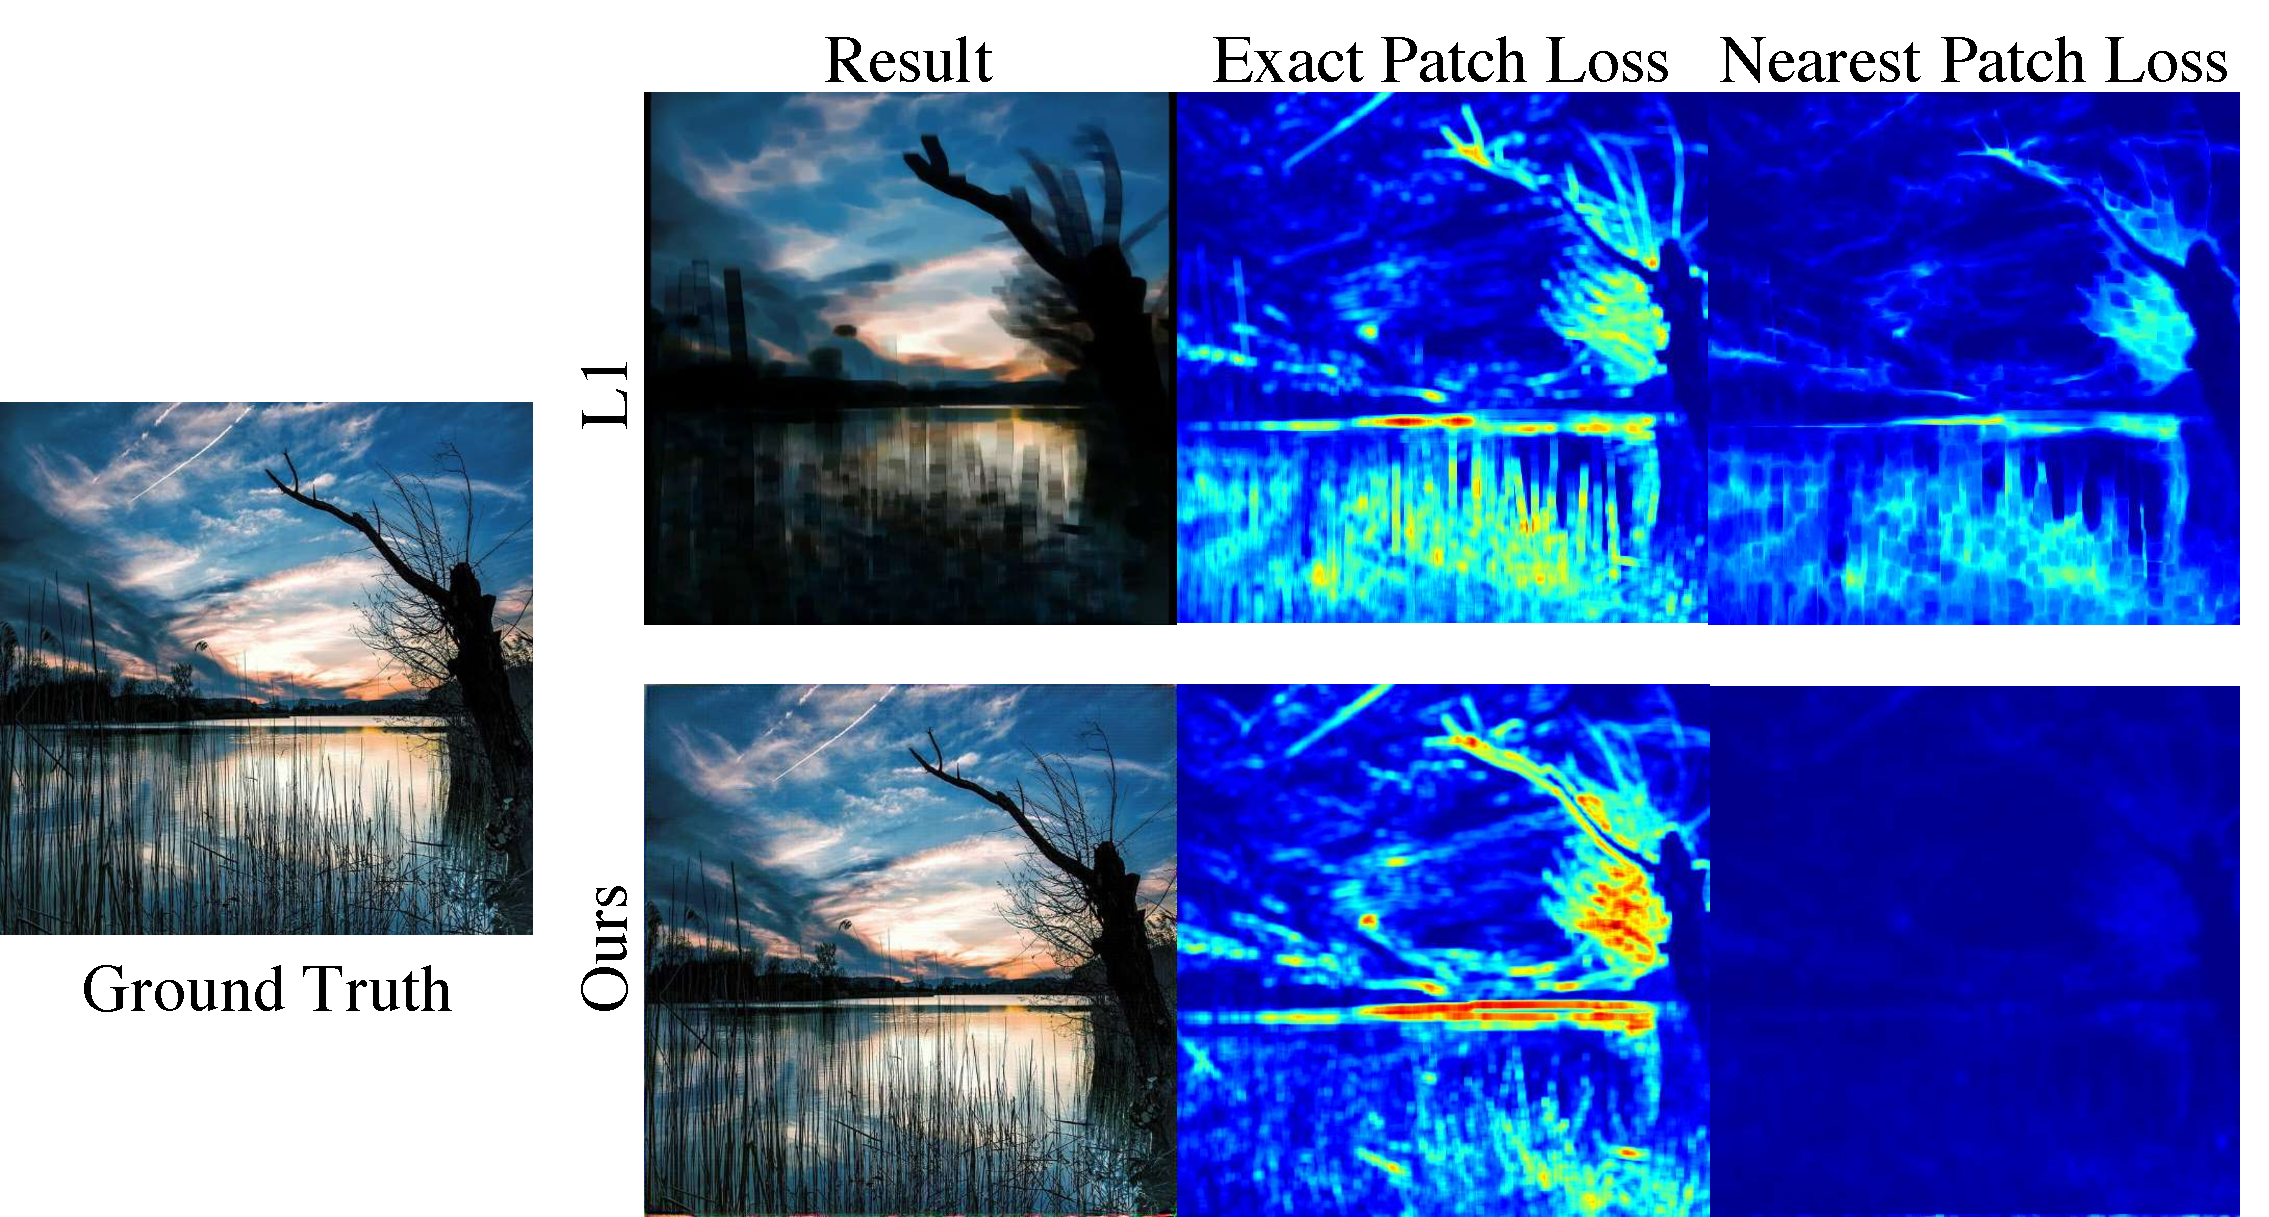
\includegraphics[width=0.8\linewidth]{texturegen/figures/exp2d.pdf}
    \caption{Texture Generation on 2D. The texture provided by our approach is visually closer to the ground truth image while avoiding blurring artifacts such as those introduced by an L1 loss.
    An exact patch loss favors alignment over perceptual similarity, while the nearest patch loss is a more robust metric.
    %Evaluated by exact patch loss, optimization based on L1 loss achieves 10.7 while ours is 11.3. Evaluated by nearest patch loss, L1 achieves 7.33 while ours is 1.53.
    }
    \label{fig:3dlite-2d-example}
\end{figure}

Visually, our optimized image is sharper and perceptually closer to the ground truth while an  L1 loss results in blurry effect from aggregating multiple misaligned observations. 
In this simple setting, we evaluate the exact patch loss for each pixel quantitatively as the L2 distance of patches centered at this pixel between the generated image and the same one in the ground truth. The exact overall exact patch loss is the L2 norm of exact patch losses for all pixels. We additionally evaluate the nearest patch loss.
Optimization with the L1 loss achieves 10.7 exact patch loss while ours is 11.3. However, we achieve 1.53 nearest patch loss, which is smaller than L1 as 7.33. This suggests that our method prefers realistic misalignment to blur. We successfully derive an image where every local patch is nearly identical to a misaligned version of the patch in the ground truth image.

\paragraph*{Synthetic 3D Example}
%\paragraph*{Robust to Camera or Geometry Errors?}
In order to quantitatively evaluate our 3D texture generation, we create a synthetic dataset of 16 models randomly selected from ShapeNet~\cite{chang2015shapenet} across different categories. 
These shapes typically contain sharp edges and self-occlusion boundaries, complexities reflecting those of real-world objects.
Since we aim to address arbitrary texturing, we enrich the appearance of these shapes by using 16 random color images from the internet as texture images. 
To create  virtual scans of the objects, we uniformly sample $>900$ views on a unit hemisphere by subdividing an icosahedron, from which we render the textured geometry as observed color images. 
To simulate misalignment, we associate each rendered image with a slightly perturbed camera pose, and to simulate geometry errors, we apply random perturbations to the geometric model.
We use a set of errors increasing from $n=1$ to $n=4.5$, and refer to the supplemental material for additional detail regarding generating camera and geometry perturbations.


In Table~\ref{tab:toptim-cam-err}, we study the effect of varying camera and geometry errors in this synthetic 3D setting.  We report evaluation metrics for our approach as well as several state-of-the-art texture optimization methods, including methods based on an L1 loss and texturing using sharpest frame selection~\cite{vu2011bf}.
Our approach outperforms all other methods, as it avoids blurring effects often seen with L1 and ColorMap~\cite{zhou2014color}, and it avoids seams and over-sharpness introduced by methods relying on sharpness selection (3DLite~\cite{huang20173dlite} and sharpest frame selection).
VGG~\cite{johnson2016perceptual} aggregates views by blending deep features, which is insufficient for handling misalignment artifacts.
Two example scenes with increasing errors in camera and geometry are shown in Figure~\ref{fig:toptim-pose-visual}.

\begin{table}
    \centering
    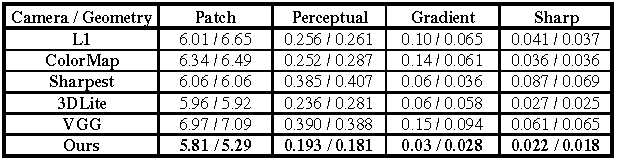
\includegraphics[width=0.8\linewidth]{texturegen/figures/synthetic-table.pdf}
    \caption{Evaluation of different methods on our 3D synthetic dataset averaged across different levels of camera pose and geometry errors.}
    \label{tab:toptim-cam-err}
\end{table}
\begin{figure}
\begin{minipage}{0.49\linewidth}
    \centering
    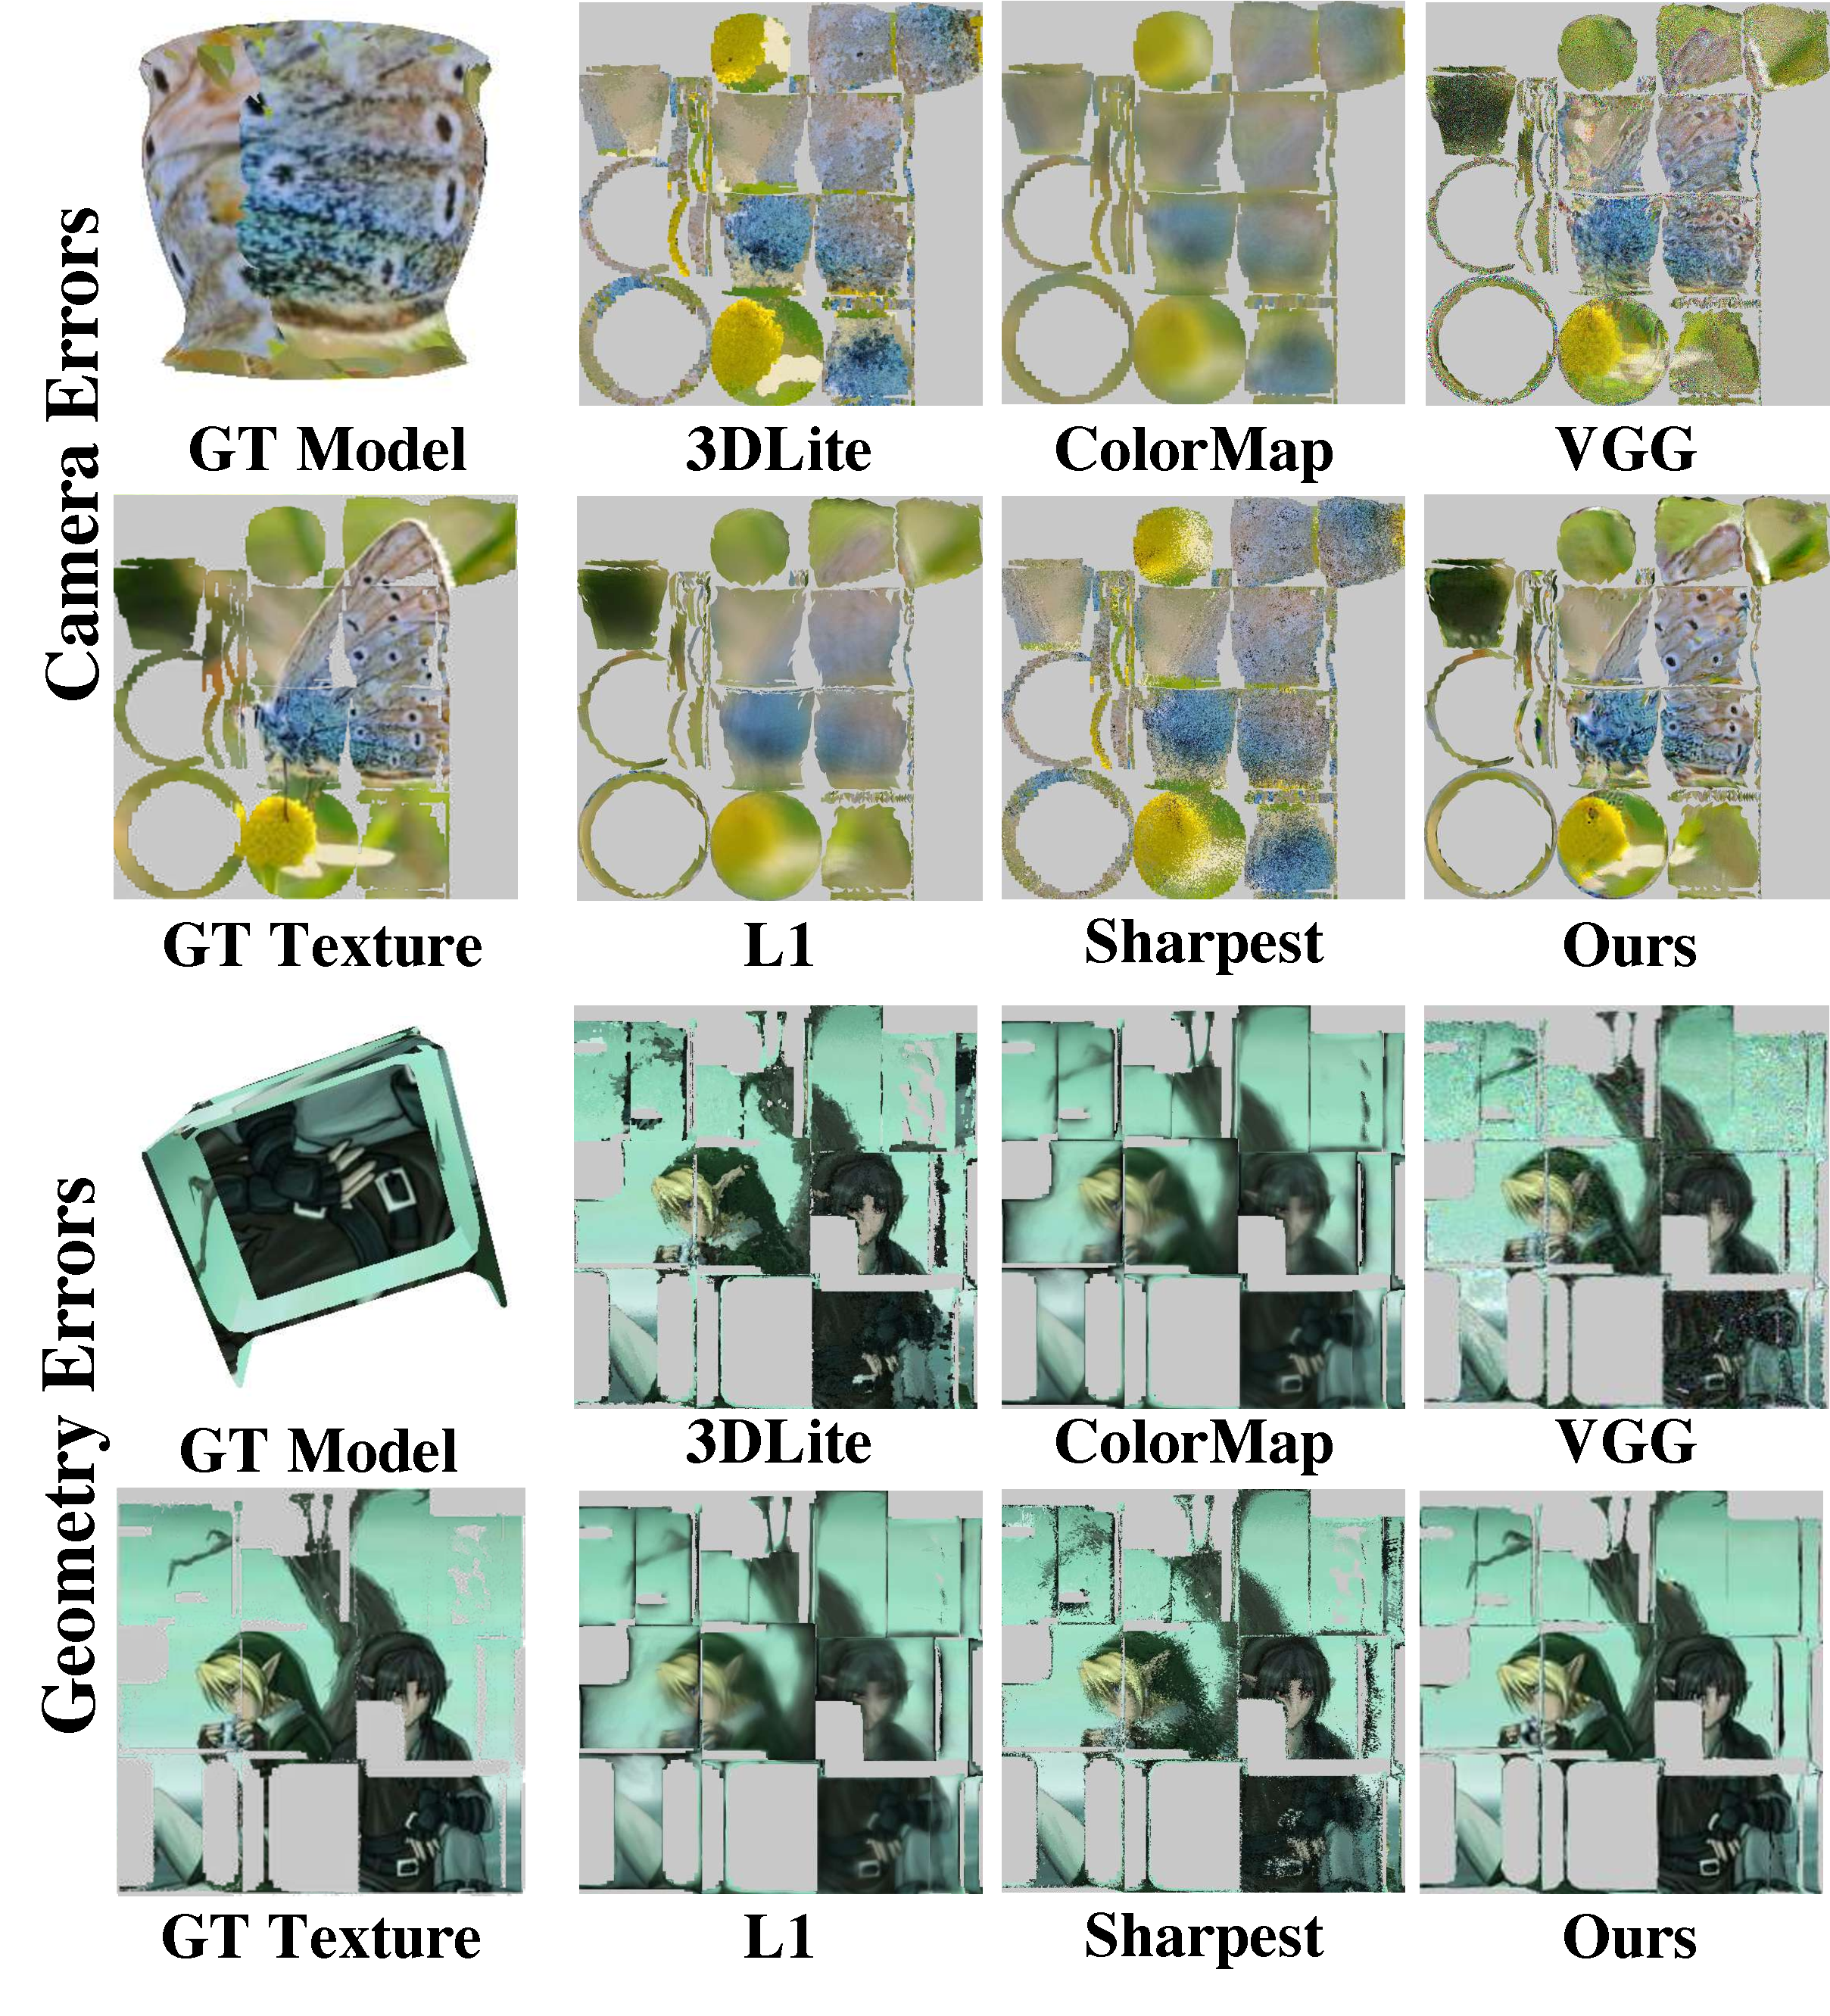
\includegraphics[width=\linewidth]{texturegen/figures/synth-results.pdf}
    \caption{Texture generation in case of high camera or geometry errors. ColorMap~\cite{zhou2014color} cannot handle such large errors. Sharpest or 3DLite~\cite{huang20173dlite} selection leads to inconsistent boundaries or breaks structures. VGG~\cite{johnson2016perceptual} aggregates views by blending deep features with noises, which is not sufficient for handling misalignment artifacts. Ours is visually closest to the ground truth.}
    \label{fig:toptim-pose-visual}
\end{minipage}
\begin{minipage}{0.49\linewidth}
\begin{minipage}{\linewidth}
    \centering
    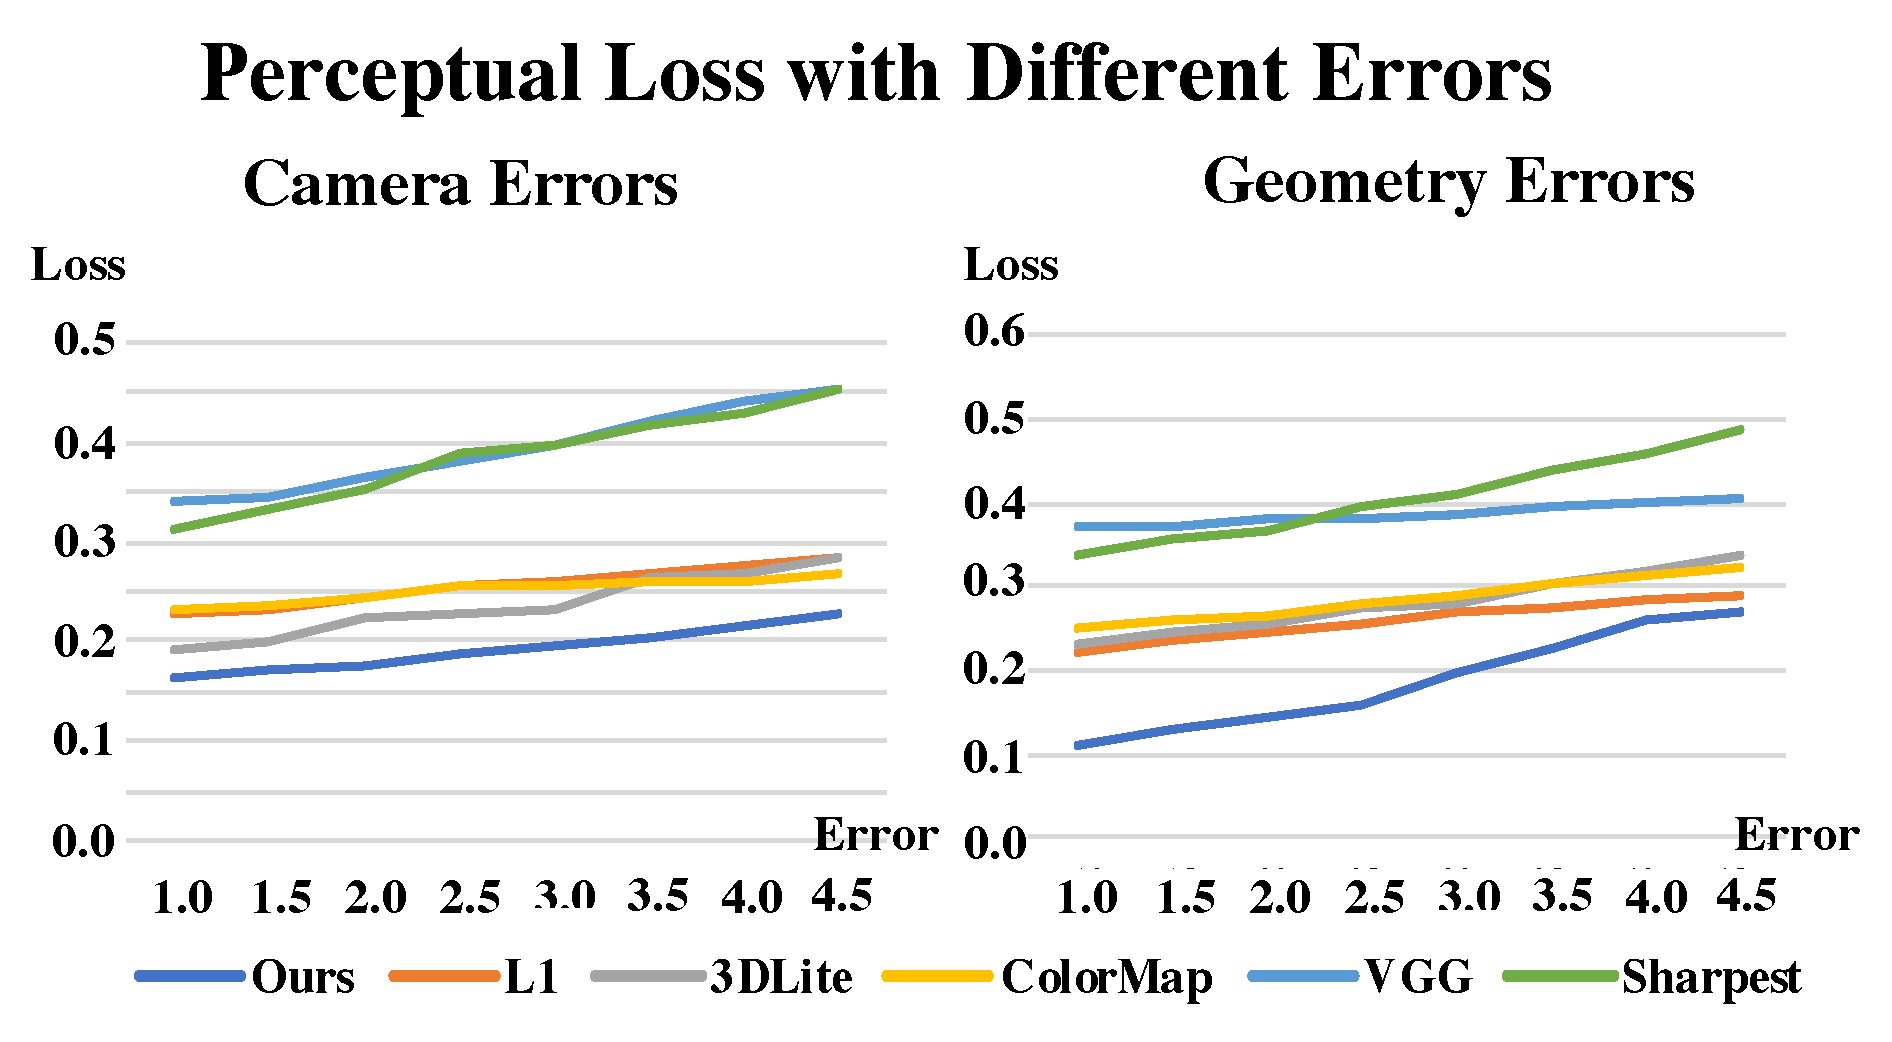
\includegraphics[width=0.9\linewidth]{texturegen/figures/chart.pdf}
    \caption{Perceptual loss of different approaches under increasing camera or geometry errors. Ours outperforms existing methods in different levels of errors.}
    \label{fig:toptim-pose-chart}
\end{minipage}
\begin{minipage}{\linewidth}
    \centering
    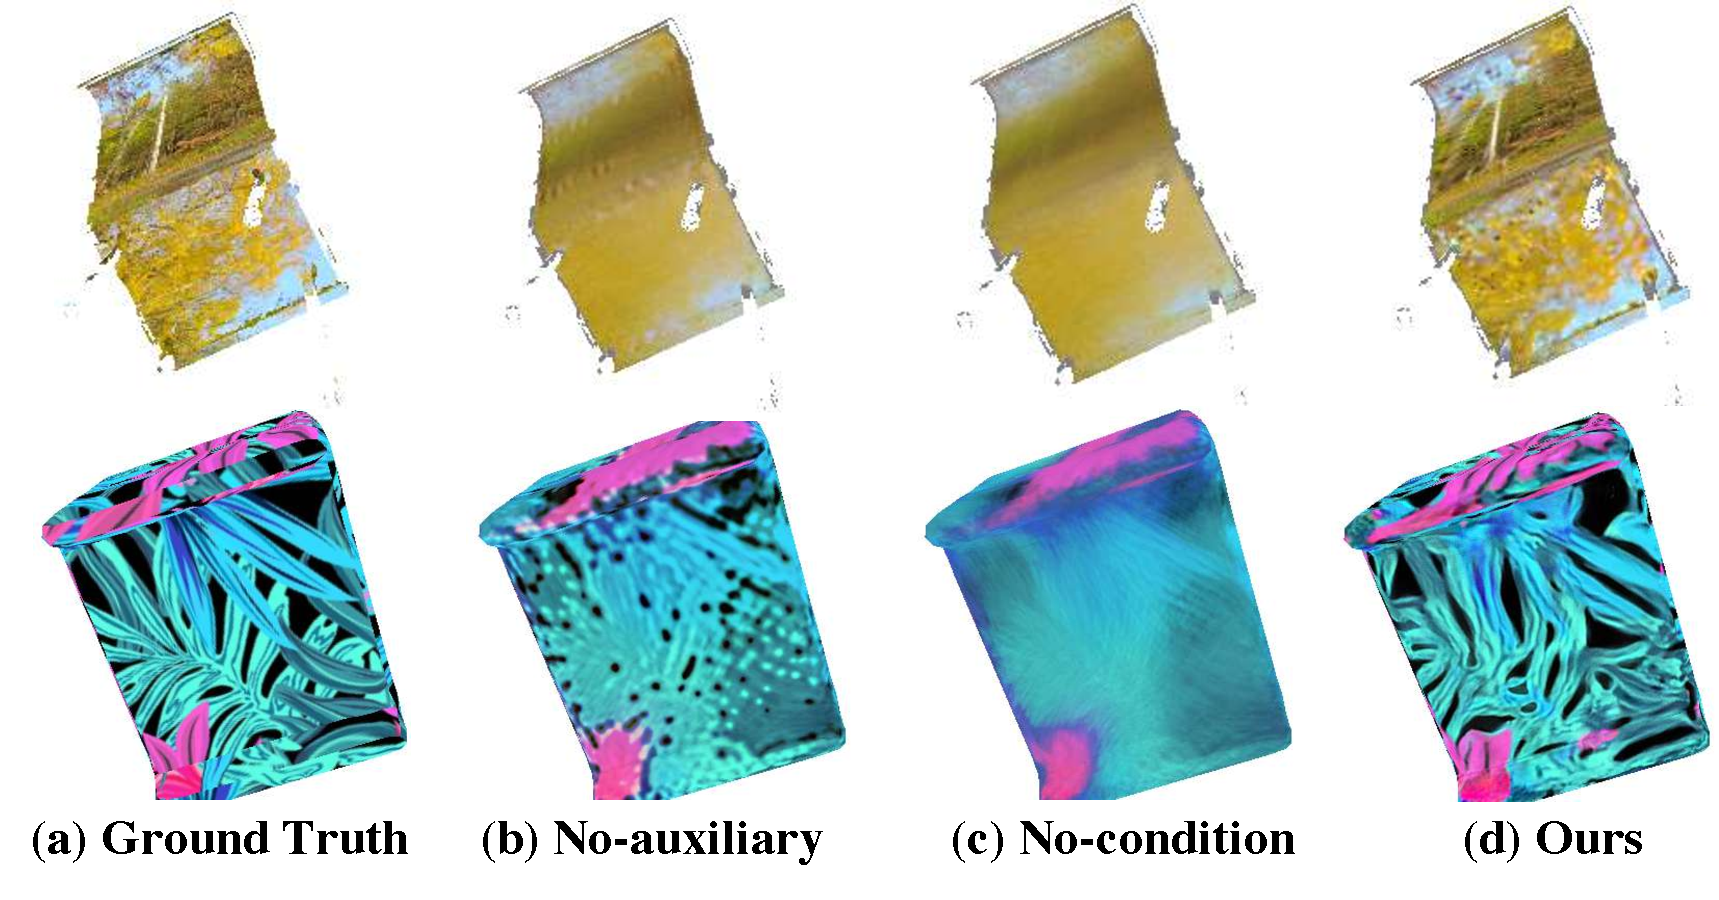
\includegraphics[width=\linewidth]{texturegen/figures/adversarial-compare.pdf}
    \caption{Comparing different discriminator options. (b) removes the auxiliary view from the discriminator, resulting in the lack of robustness to misalignments. (c) removes the condition from the discriminator, resulting in ambiguity in local regions. (d) our conditional discriminator leveraging auxiliary views to provide examples of realistic misalignments enables tolerance to misalignment and generation of textures reflecting input image characteristics. }
    \label{fig:toptim-gan-err}
\end{minipage}
\end{minipage}
\end{figure}

We additionally study the behavior of all methods in this experiment using the perceptual metric~\cite{zhang2018unreasonable} in Figure~\ref{fig:toptim-pose-chart}.
Although the performance drops for all methods with the increase of camera/geometry errors, our approach maintains the best perceptual quality as the errors increase. Visualization of several textured models generated by ColorMap~\cite{zhou2014color} and ours are shown in Figure~\ref{fig:toptim-pose-chart}; our approach maintains a sharp result while ColorMap produces increasingly blurriness as the error increases. 

\begin{figure}
    \centering
    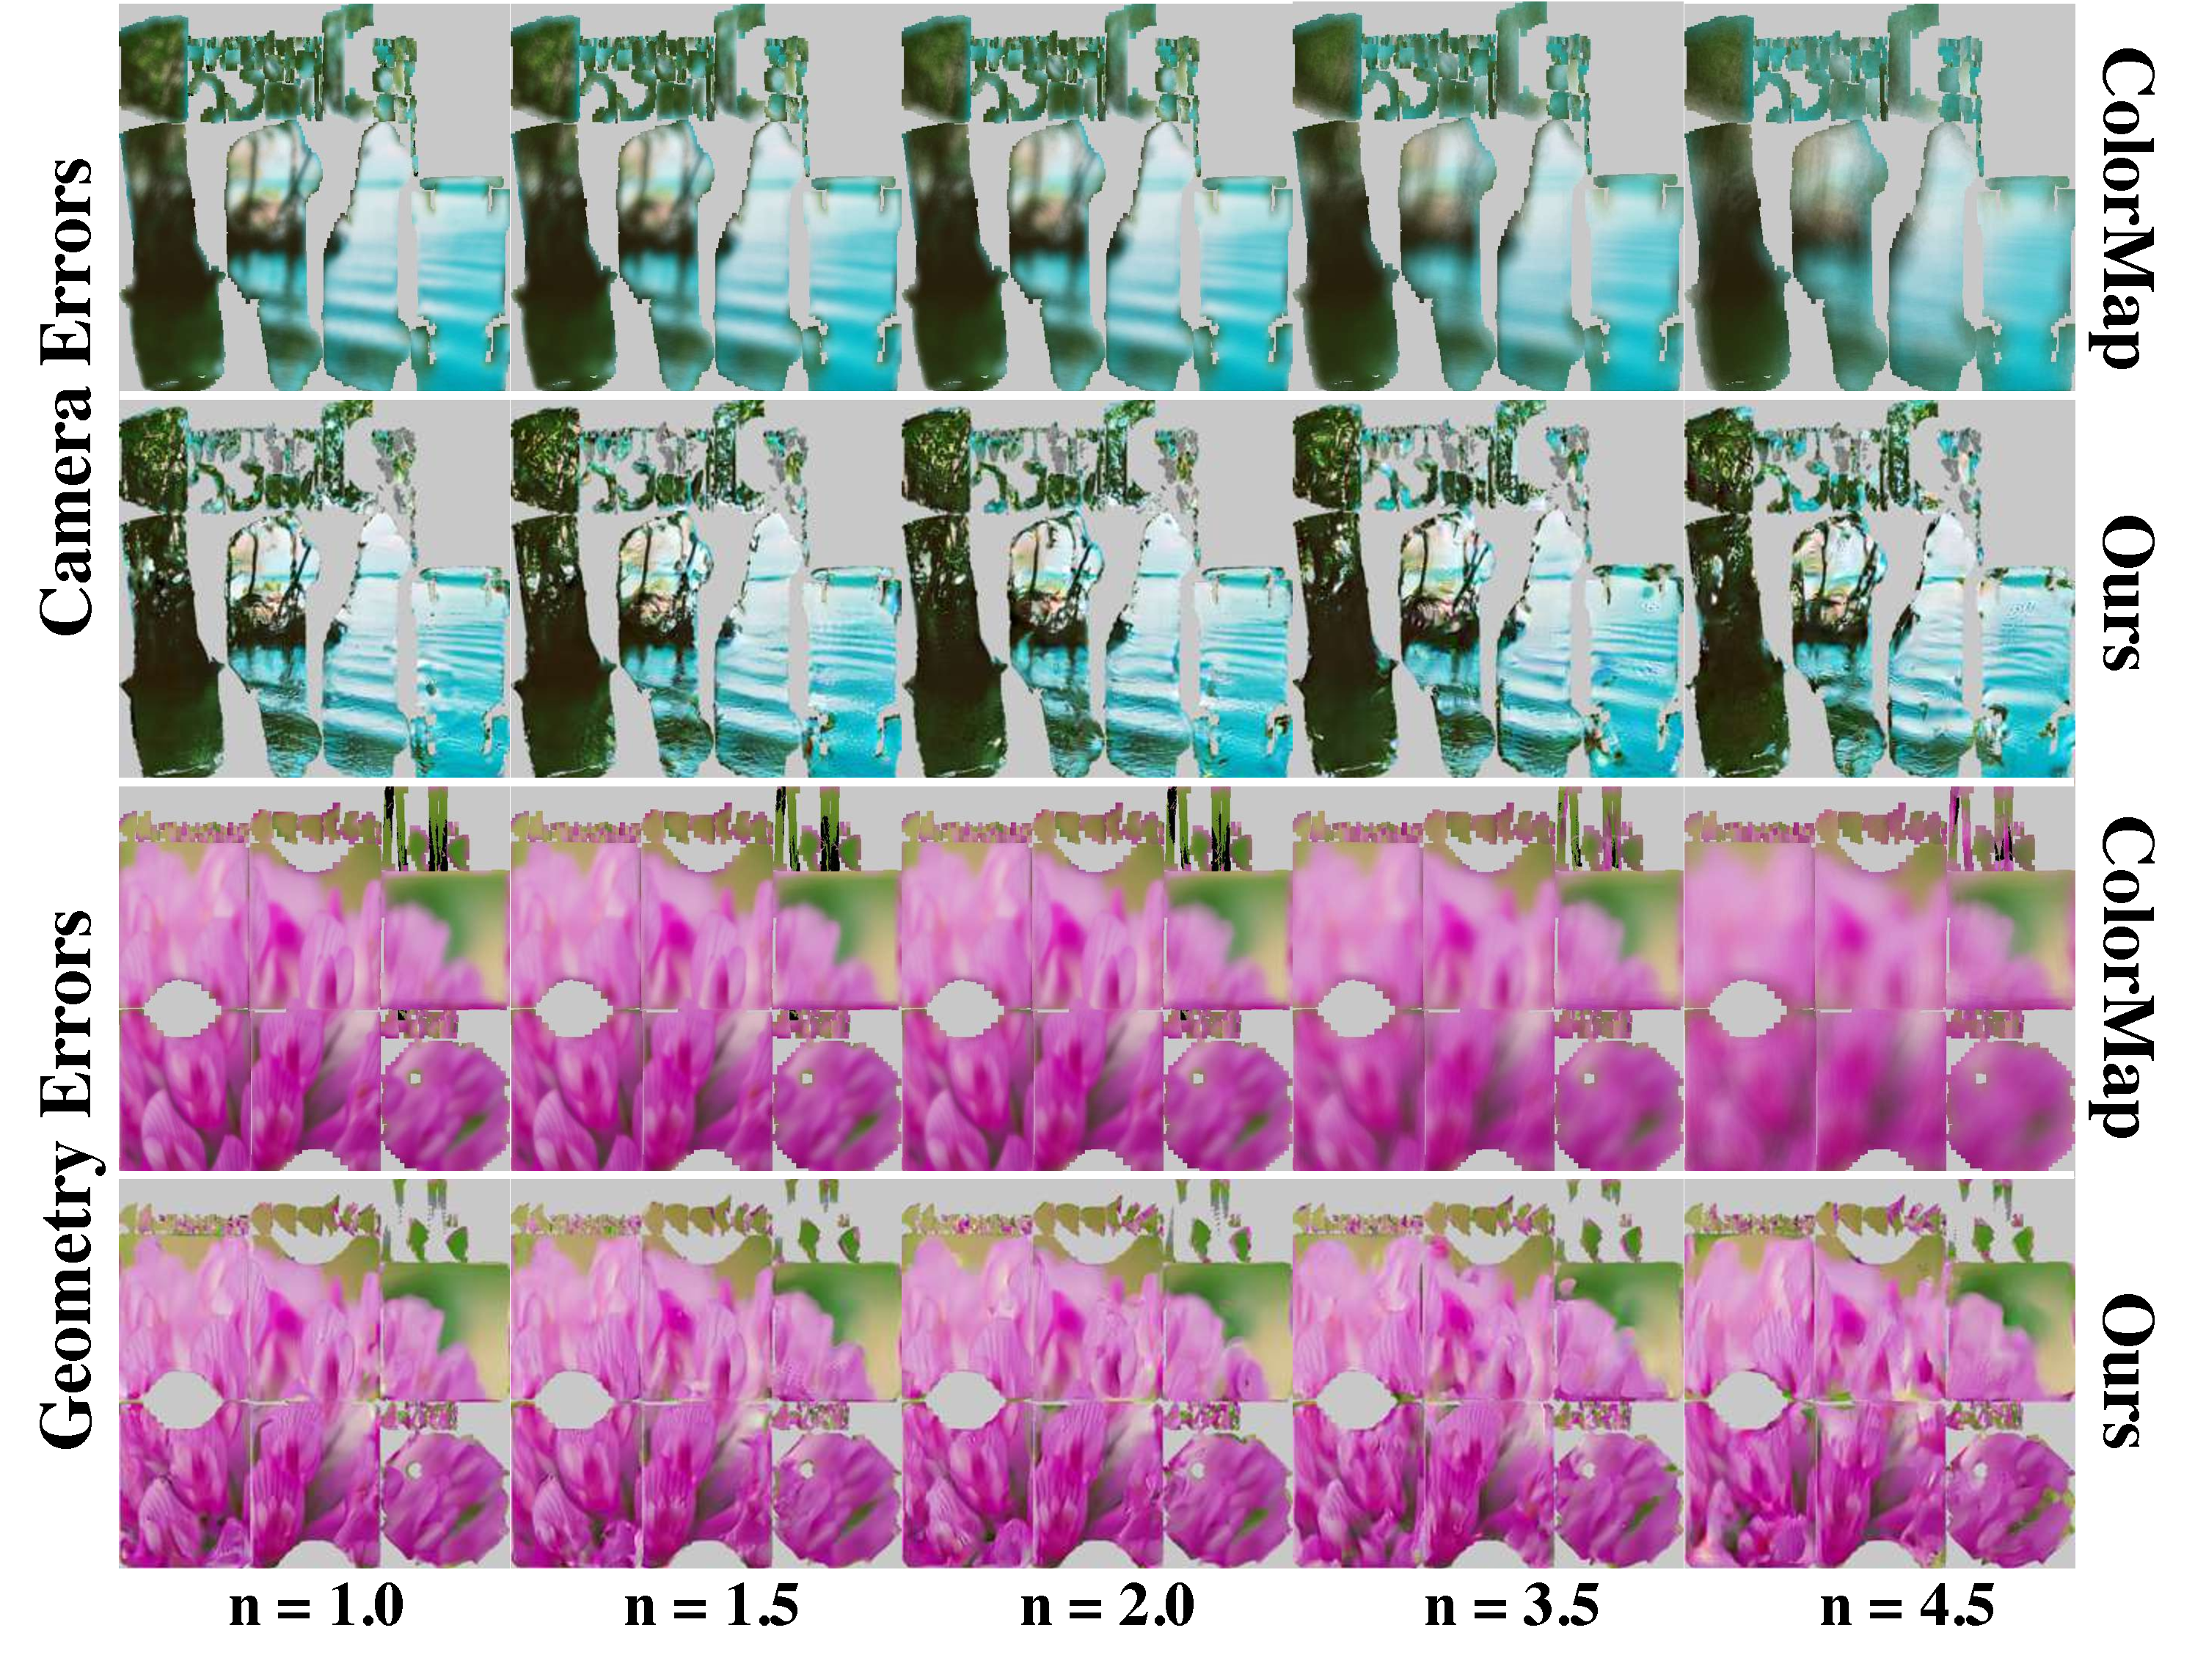
\includegraphics[width=0.8\linewidth]{texturegen/figures/results-synth-diff.pdf}
    \caption{Visualization of texture generation under increasing camera or geometry errors. Under the increase of camera pose/geometry errors, ColorMap~\cite{zhou2014color} produces more blurry results while ours maintains sharp textures.}
    \label{fig:pose-diff}
\end{figure}

\paragraph*{Alternative Choices for Discriminators?} 
We analyze the design choices for our misalignment-tolerant conditional discriminator in Figure~\ref{fig:toptim-gan-err}.
Removing the auxiliary view (b) and thus relying only on the source view to provide `real' examples to the discriminator (similar to pix2pix~\cite{isola2017image}) renders the metric unable to handle misalignments.
We also evaluate a  general discriminator that classifies whether a generated patch is real or fake among entire input view sets without any condition (c), resulting in ambiguity regarding where real patches come from. 
Our conditional discriminator leveraging reprojected auxiliary views enables robustness to misalignment, resulting in realistic texturing.

\paragraph*{Real Object Scans}
We compare our method to state-of-the-art texturing methods on scanned objects from real environments. We use a structure sensor\footnote{https://structure.io} along with its SLAM system to scan 35 chairs, producing scanned geometry, RGB-D frames and the camera poses ($\approx 500$ frames per scan). 
The foreground/background for the object in the RGB frames is determined by whether a ray intersects with the reconstructed geometry. Figure~\ref{fig:toptim-object-scan} (rows 1-4) shows qualitative comparisons.
With an L1 loss or ColorMap~\cite{zhou2014color}, blur artifacts are induced by misalignment errors.
Sharpest selection and 3DLite~\cite{huang20173dlite} use sharp region selection, resulting in seams and inconsistent global structures, as shown in the flower, leaf, and chair arms. 
A VGG loss~\cite{johnson2016perceptual} produces excess noise artifacts.  
Our approach produces sharp and consistent texturing, including detailed patterns such as the leaves in row 1 and woven structures in rows 2 and 3.

Additionally, we show a quantitative evaluation in Table~\ref{tab:toptim-result} (first column) by evaluating the perceptual metric~\cite{zhang2018unreasonable} for rendered textures against input observed views; our approach achieves the most realistic texturing.

\paragraph*{Real Scene Scans}
To demonstrate the capability of our approach to optimize texture on a larger scale, we run our algorithm on the ScanNet dataset~\cite{dai2017scannet}, which provides RGB-D sequences and reconstructed geometry of indoor scenes.
We evaluate our approach on scenes with ID $\leq 20$ ($\approx 2000-3000$ frames per scan) and compare it with the existing state of the arts. 
Figure~\ref{fig:toptim-object-scan} (rows 5-9) and Table~\ref{tab:toptim-result} (middle column) show qualitative and quantitative comparisons. 
Our method produces texturing most perceptually similar to the observed images; our misalignment-tolerant metrics aids in avoiding blur, increased sharpness, or excess noise produces by other methods due to camera and geometry errors in real-world scans.
%We achieve better visual result compared to all other approaches with sharper or more consistent textures. Figure~\ref{fig:toptim-object-scan} (row 5-9) shows a visual comparison among different methods, where our result looks closest to the ground truth images.

\paragraph*{Real to CAD Models}
Since our method can better handle errors due to approximate surface geometry, it is possible to consider texturing CAD models using real-world images to attain realistic appearances.   While large datasets of 3D CAD models are now available~\cite{chang2015shapenet}, they are often untextured or textured simplistically, resulting in notably different appearance from real-world objects. 
To test whether our method can be applied in this challenging scenario, 
%We thus apply our approach to texturing CAD models using real-world imagery, to provide more realistic appearance despite both differing geometry of synthetic CAD models and real-world objects as well as camera errors in captured imagery. To this end, 
we use our collected dataset of real object scans, retrieve similar CAD models from ShapeNet~\cite{chang2015shapenet}, and rigidly align them to the scanned objects.
We then replace the scanned geometry with the CAD model geometry and then use the captured color images and estimated poses from the scan to optimize the CAD texture.
Qualitative and quantitative evaluation of our approach in comparison to existing state-of-the-art methods are show in Figure~\ref{fig:toptim-object-scan} (rows 10-13) and Table~\ref{tab:toptim-result} (right column), respectively.
Our approach is able to handle both camera poses errors as well as the synthetic-real geometry differences to produce texturing perceptually very similar to observed imagery, whereas other methods suffer strong blur, noise, and seam artifacts under these errors.
%, it opens the potential for attaching real world appearance to the CAD models. We manually find the chairs as CAD models in ShapeNet which looks similar to the scanned model and apply a rigid 3D transformation to roughly align them. Then, we replace the scanned geometry with the CAD model and aim at mapping the color information from the scanning video to it. Figure~\ref{fig:toptim-object-scan} (row 10-13) shows the results from different approaches on painting CAD models. Our approach produces minimum artifacts and faithfully paint textures on top of the CAD models.

\paragraph*{Evaluation}
\begin{figure}
\begin{minipage}{0.49\linewidth}
    \centering
    \begin{tabular}{|c|c|c|c|}
        \hline
        & Object & ScanNet & CAD\\
        \hline
        L1 & 0.197 & 0.470 & 0.199 \\
        \hline
        ColorMap & 0.186 & 0.461 & 0.234 \\
        \hline
        Sharpest & 0.222 & 0.510 & 0.260 \\
        \hline
        3DLite & 0.185 & 0.445 & 0.238 \\
        \hline
        VGG & 0.272 & 0.534 & 0.289 \\
        \hline
        Ours & \textbf{0.175} & \textbf{0.395} & \textbf{0.176} \\
        \hline
    \end{tabular}
    \captionof{table}{Mean perceptual loss comparing the input images and rendered textures from different methods. Our method achieves best performance in the real and CAD datasets.}
    \label{tab:toptim-result}
\end{minipage}
\begin{minipage}{0.49\linewidth}
    \centering
    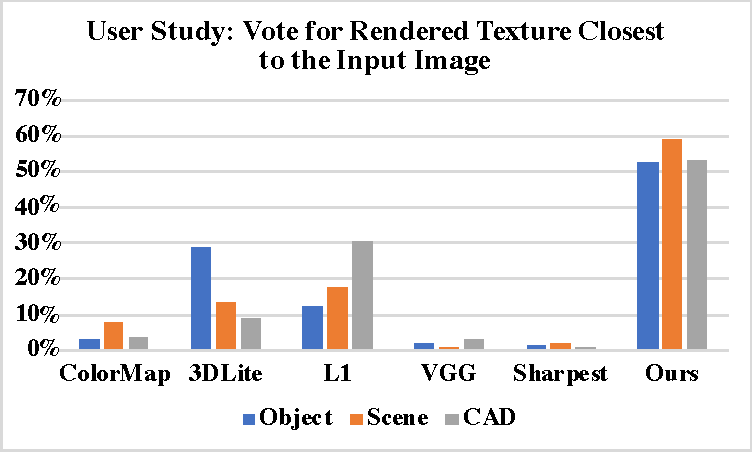
\includegraphics[width=0.8\linewidth]{texturegen/figures/user.pdf}
    \caption{User study. We ask people to vote for the rendered textures from different methods that look closest to the input image.}
    \label{fig:user-study}
\end{minipage}
\end{figure}
Although we lack ground truth texturing for the objects in the real environments, we can compare the perceptual loss~\cite{zhang2018unreasonable} with the rendering of textured geometry at the corresponding viewpoint. We select 10 views uniformly distributed from the scanning video, render the textured model to compute the mean of the perceptual loss.
Table~\ref{tab:toptim-result} shows the performance of different methods on the object scans, scene scans and the CAD models, and our method achieves the best performance in these three scenarios.

Additionally, we perform a user study to evaluate the quality of the texture, shown in Figure~\ref{fig:user-study}.
Our user study comprised $63$ participants who were asked to vote for the texture which produced a rendering closest to the input image. 
For some views, it can sometimes be difficult for users to differentiate between different methods when regions are largely uniform in color. 
Nevertheless, our method is  still notably preferred over other texturing approaches.
\begin{figure}
    \centering
    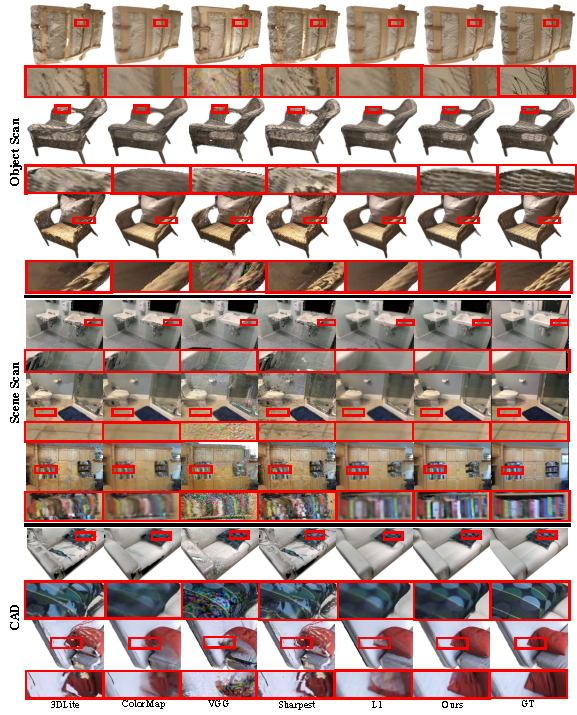
\includegraphics[width=\linewidth,height=1.15\linewidth]{texturegen/figures/result.pdf}
    \caption{Visual comparison on object scans, ScanNet~\cite{dai2017scannet} scans of scenes, and CAD models aligned with object scans. Due to misalignment errors in both camera pose and geometry, both L1 loss and ColorMap~\cite{zhou2014color} produce blurry artifacts, sharpest selection and 3DLite~\cite{huang20173dlite} result in inconsistent regions or breaks in texture structure, and VGG~\cite{johnson2016perceptual} blends learned features resulting in structural artifacts and noise. Our misalignment-tolerant approach produces sharp and consistent textures.}
    \label{fig:toptim-object-scan}
\end{figure}